% =====================================================================
%  CLD 880 - Minor Project Report  (COMPRESSED — target 20-22 pp)
%  Sakhare Yash Balram, 2022CH71496
%  Department of Chemical Engineering, IIT Delhi
% =====================================================================

\documentclass[10pt,a4paper]{article}

% - core typesetting -
\usepackage[T1]{fontenc}
\usepackage{lmodern}
\usepackage[utf8]{inputenc}
\usepackage{microtype}
\DisableLigatures[-]{encoding = T1, family = *}
\usepackage[english]{babel}
\usepackage{geometry}
\geometry{a4paper,top=15mm,bottom=15mm,left=17mm,right=17mm}
\usepackage{setspace}
\setstretch{1.08}

% Tight paragraph and list spacing
\setlength{\parskip}{0.5pt plus 0.5pt minus 0pt}
\setlength{\parindent}{1.0em}
\usepackage{enumitem}
\setlist{topsep=0pt,itemsep=0pt,parsep=0pt,leftmargin=1.4em}

% - math & units -
\usepackage{amsmath}
\usepackage{amssymb}
\usepackage{siunitx}
\sisetup{detect-all,per-mode=symbol}

% - figures, tables, captions -
\usepackage{graphicx}
\usepackage{float}
\usepackage{subcaption}
\usepackage{booktabs}
\usepackage[font=scriptsize,labelfont=bf,labelsep=period,skip=2pt]{caption}
\setlength{\textfloatsep}{3pt plus 1pt minus 1pt}
\setlength{\intextsep}{3pt plus 1pt minus 1pt}
\setlength{\abovecaptionskip}{2pt}
\setlength{\belowcaptionskip}{0pt}

% - section headings -
\usepackage[explicit]{titlesec}
\titleformat{\section}{\sffamily\large\bfseries}{\thesection.}{0.5em}{#1}
\titleformat{\subsection}{\sffamily\normalsize\bfseries}{\thesubsection.}{0.5em}{#1}
\titleformat{\subsubsection}{\sffamily\normalsize\itshape}{\thesubsubsection.}{0.5em}{#1}
\titleformat{\paragraph}[runin]{\sffamily\normalsize\bfseries}{}{0pt}{#1}
\titlespacing*{\section}{0pt}{6pt plus 2pt minus 1pt}{3pt plus 1pt}
\titlespacing*{\subsection}{0pt}{4pt plus 2pt minus 1pt}{2pt plus 1pt}
\titlespacing*{\subsubsection}{0pt}{3pt plus 1pt}{1pt}

% - bibliography -
\usepackage[numbers,sort&compress,square]{natbib}

% - hyperlinks -
\usepackage[hidelinks,unicode=true,psdextra=true]{hyperref}
\pdfstringdefDisableCommands{%
  \def\Hi{H2}%
  \def\CHi{CH4}%
  \def\dD{d/D}%
  \def\VR{VR}%
  \def\HBR{HBR}%
  \def\CoV{CoV}%
  \def\Ri{Ri}%
  \def\Frnum{Fr}%
  \def\^#1{#1}%
  \def\circ{ deg}%
}

% - helpers -
\usepackage{xcolor}
\newcommand{\Hi}{\ensuremath{\mathrm{H_2}}}
\newcommand{\CHi}{\ensuremath{\mathrm{CH_4}}}
\newcommand{\dD}{\ensuremath{d/D}}
\newcommand{\VR}{\ensuremath{\mathrm{VR}}}
\newcommand{\HBR}{\ensuremath{\mathrm{HBR}}}
\newcommand{\CoV}{\ensuremath{\mathrm{CoV}}}
\newcommand{\Ri}{\ensuremath{\mathrm{Ri}}}
\newcommand{\Frnum}{\ensuremath{\mathrm{Fr}}}

\title{}
\author{}
\date{}

\begin{document}
\small

% =====================================================================
%  TITLE PAGE
% =====================================================================
\begin{titlepage}
    \centering
    \vspace*{0.3cm}
    {\normalsize \bfseries Minor Project Report \par}
    \vspace{0.1cm}
    {\normalsize \bfseries CLD\,880 \par}
    \vspace{0.8cm}

    {\Large \bfseries Multiobjective Optimization of \\[0.1cm]
    Hydrogen Injection into High-Pressure \\[0.1cm]
    Natural Gas Pipelines \par}

    \vspace{0.3cm}
    {\normalsize \bfseries A Surrogate-Assisted Multi-Objective Approach \par}

    \vspace{0.8cm}
    {\normalsize Submitted by \par}
    \vspace{0.15cm}
    {\large \bfseries Sakhare Yash Balram \par}
    {\normalsize 2022CH71496 \par}

    \vspace{0.5cm}
    {\normalsize Under the supervision of \par}
    \vspace{0.15cm}
    {\large \bfseries Prof.~Abhijeet Raj \par}

    \vspace{0.6cm}
    \IfFileExists{logos/IITD_Logo_Big.jpg}{%
        
\includegraphics[width=0.18\textwidth]{logos/IITD_Logo_Big.jpg}%
    }{%
        \IfFileExists{logos/IITD_Logo_Big.png}{%
            
\includegraphics[width=0.18\textwidth]{logos/IITD_Logo_Big.png}%
        }{%
            \fbox{\parbox[c][2cm][c]{0.25\textwidth}{\centering\itshape\scriptsize
                IITD logo}}%
        }%
    }\par
    \vspace{0.4cm}

    {\normalsize \bfseries Department of Chemical Engineering \par}
    {\normalsize \bfseries Indian Institute of Technology Delhi \par}
    {\normalsize \bfseries New Delhi - 110016 \par}
    \vspace{0.15cm}
    {\normalsize \bfseries April 2026 \par}

    \vfill
    \renewcommand{\arraystretch}{1.2}
    \begin{tabular}{|p{0.42\textwidth}|p{0.42\textwidth}|}
        \hline
        \centering \textbf{Supervisor's signature} &
        \centering \textbf{Date} \tabularnewline
        \hline
        \vspace{0.8cm} & \vspace{0.8cm} \tabularnewline
        \hline
    \end{tabular}
    \vspace*{0.1cm}
\end{titlepage}

% =====================================================================
%  ABSTRACT (condensed)
% =====================================================================
\begin{center}
    {\large \bfseries \sffamily Abstract}
\end{center}
\noindent
This work presents a CFD-based parametric study of \Hi{} injection
through a side branch into a \(\SI{0.46}{\meter}\) \CHi{} main pipe
at \(\SI{10}{\meter\per\second}\), using \texttt{rhoReactingBuoyantFoam}
(OpenFOAM) with the \(k\)-\(\omega\)~SST closure.  Three design
variables are swept: diameter ratio
\(\dD\in[0.15,\,0.45]\), velocity ratio
\(\VR\in[0.69,\,5.84]\), and injection angle
\(\alpha\in\{30^\circ,\,90^\circ\}\).  Four ten-case Latin Hypercube
campaigns (two angles \(\times\) two injection sides: top and bottom)
yield 40~valid CFD evaluations.  Mixing quality is reported as the
outlet coefficient of variation \CoV{} of the \Hi{} mass fraction;
pumping cost as the LP-filtered gauge pressure drop
\(|\Delta p_{\mathrm{rgh}}|\).

\textbf{Key findings.}
(i)~The \(30^\circ\) tilt reduces \CoV{} in all seven matched pairs
(median \(-46\,\%\)) and \(|\Delta p|\) in all seven (median
\(-63\,\%\)); (ii)~top injection is strictly superior to bottom
injection --- all 17 matched pairs show lower \CoV{} for top
(median degradation top\(\to\)bottom: \(+109\,\%\) at \(90^\circ\),
\(+324\,\%\) at \(30^\circ\)); (iii)~a Gaussian Process surrogate
achieves \(R^{2}=0.93\) for \CoV{} on leave-one-out CV, enabling
NSGA-II Pareto search; (iv)~\(\Delta p\) is unpredictable
(\(R^{2}\approx 0\)) due to acoustic noise in the compressible solver.

\vspace{0.5em}
\noindent
\textbf{Keywords:} hydrogen blending; T-junction; CFD; RANS;
\(k\)-\(\omega\)~SST; OpenFOAM; Latin Hypercube; CoV; surrogate; NSGA-II.

% =====================================================================
%  1. INTRODUCTION  (condensed: 4 subsections -> 1 section)
% =====================================================================
\section{Introduction}
\label{sec:intro}

Blending green hydrogen into existing natural-gas networks (HBNG)
is the standard transition strategy for decarbonising the gas grid
without rebuilding it
\citep{su2022prediction,arya2023multi,montanes2024comprehensive}.
The eight-to-one density ratio between \CHi{} and \Hi{}
(Table~\ref{tab:properties}) causes the lighter gas to stratify
rather than mix uniformly, with three downstream consequences:
(i)~hydrogen embrittlement of the pipe wall, since
\(p_{\Hi}^{0.5}\)-dependent cracking exposes the crown to
near-pure \Hi{} \citep{topolski2022blending};
(ii)~combustion instability at end-burners due to Wobbe-index
drift; and (iii)~metering error from composition-dependent
speed-of-sound shifts \citep{su2022prediction}.

\begin{table}[H]
\centering\scriptsize
\caption{Selected properties of \Hi{} and \CHi{} at STP.}
\label{tab:properties}
\begin{tabular}{lccl}
\toprule
\textbf{Property} & \textbf{\CHi{}} & \textbf{\Hi{}} & \textbf{Consequence} \\
\midrule
Density (kg/m\(^3\))       & 0.668 & 0.082 & \(8\times\) gap; stratification \\
Vol.\ energy (MJ/m\(^3\)) & 36 & 11 & \(3\times\) flow for same energy \\
Flammability (vol\%)       & 5--15 & 4--76 & wider explosion envelope \\
\bottomrule
\end{tabular}
\end{table}

Most parametric CFD studies fix the branch angle at
\(\alpha=90^\circ\) and sweep \(\dD\) and \(\VR\)
\citep{su2022prediction,du2024numerical,montanes2024comprehensive};
the angular sensitivity is either ignored or treated qualitatively.
Industrial siting, however, often forces non-perpendicular branch
geometries, so a quantitative angle dependence has direct
engineering value.

This project varies \((\alpha,\dD,\VR)\) on equal footing via
a sliced Latin Hypercube at \(\alpha=90^\circ\) and \(30^\circ\)
with top and bottom injection, producing 40~valid cases.
The objectives are:
\begin{enumerate}
    \item Quantify mixing (\CoV) and pumping cost (\(|\Delta p|\))
    across the design space;
    \item Compare angles and injection sides via matched-pair
    analysis;
    \item Fit a surrogate model and run NSGA-II for the
    bi-objective Pareto front.
\end{enumerate}

% =====================================================================
%  2. LITERATURE  (condensed to 1 subsection)
% =====================================================================
\section{Background and Literature Review}
\label{sec:lit}

\subsection{Stratification physics}
Whether a binary gas mixture stays mixed in a horizontal pipe is
governed by the Richardson number
\(\Ri = g\,\Delta\rho\,L / (\rho\,u^2)\).
For the present geometry (\(D=\SI{0.46}{\meter}\),
\(u=\SI{10}{\meter\per\second}\), nominal \(10\,\%\) \Hi{})
we obtain \(\Ri\sim 10^{-2}\), so the pipe-scale flow is
turbulence-dominated; buoyancy matters only \emph{locally} in
the slow shear layer downstream of the junction.
For the jet-in-crossflow problem the relevant parameter is the
momentum-flux ratio
\(J = \rho_{\mathrm{branch}}u_{\mathrm{branch}}^{2}
/ (\rho_{\mathrm{main}}u_{\mathrm{main}}^{2})\).
Intermediate \(J\) seeds the strongest counter-rotating vortex
pair, which is what we want for mixing.

\subsection{Prior CFD studies}

\paragraph{Su et al.\ (2022).}
A parametric study using Fluent with \(k\)-\(\varepsilon\) and
buoyancy \citep{su2022prediction}.  They sweep temperature,
pressure, \(\dD\) and \(\VR\) at \(\alpha=90^\circ\) and report
\CoV{} at multiple downstream stations.  \CoV{} drops
monotonically with \(\VR\) up to a knee near \(\VR\approx 2\)-\(3\).

\paragraph{Du et al.\ (2024).}
Three HBNG configurations: bare tee, bending tube, and helical
mixer \citep{du2024numerical}.  The helical mixer pushes
uniformity above \(99\,\%\) with a modest pressure penalty.

\paragraph{Monta\~n\'es et al.\ (2024).}
A reduced-order model on 26~CFD cases
\citep{montanes2024comprehensive}, recovering \CoV{} to
\(\pm 5\,\%\); the dataset is fixed at \(\alpha=90^\circ\).

\subsection{Gap addressed}
Almost the entire literature fixes \(\alpha=90^\circ\); angle
is treated as a fixed nuisance rather than a design variable.
The present project varies \((\alpha,\dD,\VR)\) on equal footing,
with matched-pair control for the angle effect.
A half-domain \texttt{symmetryPlane} simulation reproduces
full-domain results to within \(1\,\%\) and is used throughout
\citep{su2022prediction,montanes2024comprehensive}.

% =====================================================================
%  3. METHODOLOGY  (heavily condensed)
% =====================================================================
\section{Methodology}
\label{sec:method}

\subsection{Computational domain}
\label{sec:method_geom}
The geometry is a horizontal main pipe
(\(D=\SI{0.46}{\meter}\), length \(6.9\,D\); \(2.3\,D\) upstream,
\(4.6\,D\) downstream of the junction) with a branch of diameter
\(d\) (\(\dD\in[0.15,\,0.45]\)) intersecting at angle \(\alpha\).
Branch length is \(\SI{1.55}{\meter}\).
The half-domain (\(x\ge 0\)) exploits the mirror symmetry
(Fig.~\ref{fig:geometry}).
The geometry is generated parametrically
(\texttt{generateSTL.py}), reading \(\alpha\), \(d\) and \(D\) from
environment variables, and clipped to the half-space.

\begin{figure}[H]
    \centering
    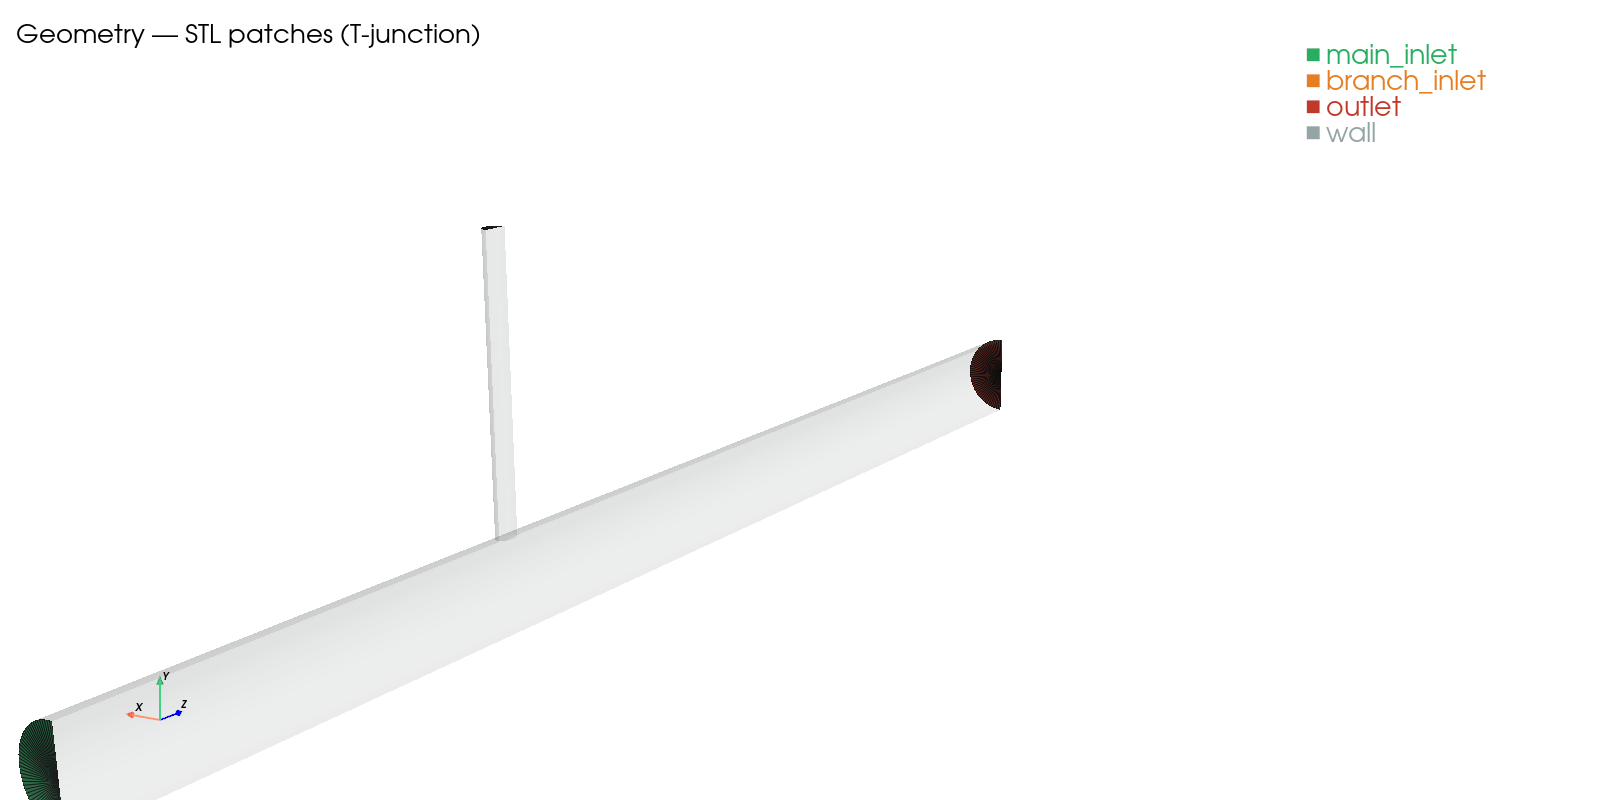
\includegraphics[width=0.75\textwidth]{../doe/results_full/cases/case_03/figures/fig_geometry.png}
    \caption{Half-domain T-junction geometry (\(90^\circ\),
    case~03, \(\dD=0.252\)).}
    \label{fig:geometry}
\end{figure}

\subsection{Governing equations}
\label{sec:method_govern}
The unsteady, compressible, multispecies Navier--Stokes equations
with gravity are solved in OpenFOAM's \texttt{rhoReactingBuoyantFoam}.
Letting \(\rho\) be the mixture density, \(\mathbf{u}\) the velocity,
\(p_{\mathrm{rgh}} = p - \rho\,\mathbf{g}\!\cdot\!\mathbf{x}\) the
modified pressure, \(h\) the sensible enthalpy and \(Y_k\) the mass
fraction of species \(k\):
\begin{align}
\frac{\partial\rho}{\partial t} +
\nabla\!\cdot\!(\rho\,\mathbf{u}) &= 0,
\label{eq:cont}\\[2pt]
\frac{\partial(\rho\mathbf{u})}{\partial t} +
\nabla\!\cdot\!(\rho\,\mathbf{u}\!\otimes\!\mathbf{u})
&= -\nabla p_{\mathrm{rgh}}
- (\mathbf{g}\!\cdot\!\mathbf{x})\nabla\rho
+\nabla\!\cdot\!\overline{\overline{\boldsymbol{\tau}}},
\label{eq:mom}\\[2pt]
\frac{\partial(\rho Y_k)}{\partial t} +
\nabla\!\cdot\!(\rho\,\mathbf{u}\,Y_k)
&=\nabla\!\cdot\!\left[\rho\!\left(D_k+\frac{\mu_t}{\mathrm{Sc}_t}\right)
\nabla Y_k\right],\quad k = \Hi,\,\CHi.
\label{eq:species}
\end{align}
Only \(Y_{\Hi}\) is solved explicitly (\(Y_{\CHi}=1-Y_{\Hi}\));
density follows the ideal-gas law.

\subsection{Turbulence closure: \texorpdfstring{$k$-$\omega$~SST}{k-omega SST}}
\label{sec:method_turb}
The Reynolds stresses are closed with the \(k\)-\(\omega\)~SST model
\citep{menter1994sst}, which blends near-wall \(k\)-\(\omega\) with
free-shear \(k\)-\(\varepsilon\) through a blending function.
Buoyancy production is enabled because the local Richardson number
can reach \(\mathcal{O}(1)\) in the shear layer downstream of the
junction.  SST is preferred over \(k\)-\(\varepsilon\)
\citep{su2022prediction} because (i) the density contrast generates
separation on the branch entry, and (ii) the near-wall layer is
resolved to \(y^+\sim 1\).

\subsection{Solver and discretisation}
\label{sec:method_solver}
\texttt{rhoReactingBuoyantFoam} uses PIMPLE (1~outer, 2~inner
correctors).  Time discretisation is implicit Euler; spatial
discretisation is second-order central (diffusion) and bounded
second-order upwind (advection); vanLeer TVD for \(Y_{\Hi}\).
Adaptive time stepping with \(\mathrm{Co}_{\max}=4.5\) (\(90^\circ\))
and \(8.0\) (\(30^\circ\)).
The full settings are in Table~\ref{tab:numerics}.

\begin{table}[H]
\centering\scriptsize
\caption{Numerical settings.}
\label{tab:numerics}
\begin{tabular}{lc}
\toprule
\textbf{Quantity} & \textbf{Choice} \\
\midrule
P-V coupling & PIMPLE (1 outer, 2 inner) \\
Time & implicit Euler \\
Div.\ (\(\rho\mathbf{u}\mathbf{u}\)) & bounded Gauss linear-upwind \\
Div.\ (\(\rho\mathbf{u} Y_{\Hi}\)) & bounded Gauss vanLeer \\
Adaptive \(\Delta t\) & \(\mathrm{Co}_{\max}=4.5\,(90^\circ),\;8.0\,(30^\circ)\) \\
\bottomrule
\end{tabular}
\end{table}

\subsection{Mesh}
\label{sec:method_mesh}
Three-step mesh: \texttt{blockMesh} \(\to\) \texttt{snappyHexMesh}
(feature-snap) \(\to\) boundary-layer extrusion (\(y^+\approx 1\),
expansion ratio 1.2).  Typical half-domain: \(\sim\!463\,\mathrm{k}\)
cells, max non-orthogonality \(49^\circ\), \(99.6\,\%\) layer
coverage (Fig.~\ref{fig:mesh}).

\begin{figure}[H]
    \centering
    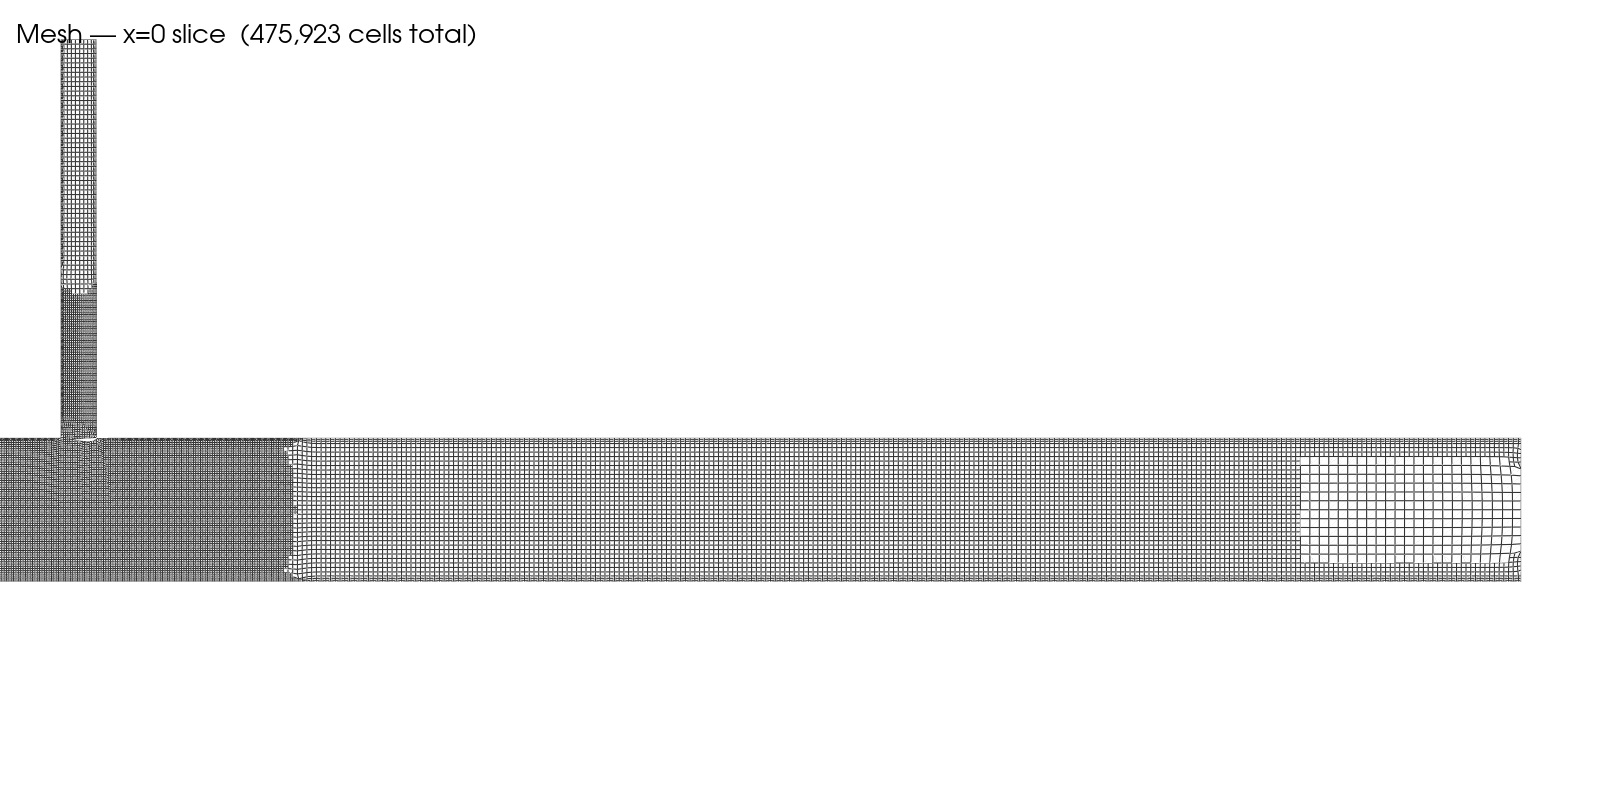
\includegraphics[width=0.75\textwidth]{../doe/results_full/cases/case_03/figures/fig_mesh_xz.png}
    \caption{Mesh cross-section on the symmetry plane (\(90^\circ\),
    case~03).}
    \label{fig:mesh}
\end{figure}

A three-level mesh-convergence study (230k / 460k / 920k cells)
at \(\dD=0.196\), \(\VR=1.64\) showed successive changes of
\(<0.5\,\%\) on \CoV{} and \(<2\,\%\) on \(|\Delta p|\)
(Table~\ref{tab:meshconv}); the 460k medium mesh was adopted.

\begin{table}[H]
\centering\scriptsize
\caption{Mesh convergence at \(\dD=0.196\), \(\VR=1.64\).}
\label{tab:meshconv}
\begin{tabular}{lcccc}
\toprule
mesh & cells & \(\Delta\CoV\) & \(\Delta|\Delta p|\) & adopted \\
\midrule
coarse & 230k & (ref.) & (ref.) & no \\
medium & 460k & 0.4\% & 1.6\% & \textbf{yes} \\
fine   & 920k & 0.2\% & 0.7\% & no \\
\bottomrule
\end{tabular}
\end{table}

\subsection{Boundary conditions}
\label{sec:method_bc}

\paragraph{\texttt{main\_inlet}.}\;
A \(1/7\)-th power-law turbulent profile with
\(u_{\mathrm{main}}=\SI{10}{\meter\per\second}\), pure \CHi{} at
\(p=\SI{6.9}{\mega\pascal}\), \(T=\SI{288}{\kelvin}\)
(\(\rho_{\mathrm{main}}\approx\SI{46}{\kilogram\per\meter\cubed}\),
\(Re_D\approx 1.7\times 10^{7}\)).
Turbulence: \(I=5\,\%\), \(\ell=0.07\,D\).

\paragraph{\texttt{branch\_inlet}.}\;
Same power-law at \(u_{\mathrm{branch}}=\VR\cdot u_{\mathrm{main}}\),
velocity vector aligned with the branch axis
\(\hat{\mathbf{s}}=(0,\sin\alpha,-\cos\alpha)\), pure \Hi{}.

\paragraph{\texttt{outlet}.}\;
Zero-gradient on \(\mathbf{u},\,Y_{\Hi},\,k,\,\omega,\,h\); fixed
total pressure on \(p_{\mathrm{rgh}}\).

\paragraph{\texttt{wall}.}\;
No-slip; \(y^+\!\approx\!1\); SST wall functions.

\paragraph{\texttt{sym}.}\;
\texttt{symmetryPlane} on \(x=0\).

\subsection{Design of Experiments (sliced LHS)}
\label{sec:method_doe}
The independent flow-and-geometry parameters at fixed angle are
\(\dD\) and \(\VR\); the hydrogen blending ratio is a derived
consequence:
\begin{equation}
\HBR = \frac{(\dD)^{2}\,\VR}{1+(\dD)^{2}\,\VR}.
\label{eq:hbr}
\end{equation}
A sliced LHS \citep{ye2000sliced} discretises \(\dD\) into 5
bins; within each, 2 \(\VR\) values are picked, giving 10~cases
per angle (Table~\ref{tab:doe_design}).
Cases sharing a \(\dD\) also share a mesh (built once per slice).
The randomisation seed is fixed across angles, so case~05 at
\(90^\circ\) and case~05 at \(30^\circ\) share all parameters
except \(\alpha\), enabling matched-pair analysis.

\begin{table}[H]
\centering\scriptsize
\caption{Ten-case sliced LHS design (shared across angles).}
\label{tab:doe_design}
\begin{tabular}{cccccc}
\toprule
case & slice & \(\dD\) & \(d\) (m) & \(\HBR\) & \(\VR\) \\
\midrule
1 & 1 & 0.196 & 0.090 & 0.184 & 5.842 \\
2 & 1 & 0.196 & 0.090 & 0.060 & 1.643 \\
3 & 2 & 0.252 & 0.116 & 0.078 & 1.330 \\
4 & 2 & 0.252 & 0.116 & 0.195 & 3.807 \\
5 & 3 & 0.296 & 0.136 & 0.098 & 1.241 \\
6 & 3 & 0.296 & 0.136 & 0.187 & 2.614 \\
7 & 4 & 0.382 & 0.176 & 0.142 & 1.137 \\
8 & 4 & 0.382 & 0.176 & 0.092 & 0.693 \\
9 & 5 & 0.396 & 0.182 & 0.130 & 0.953 \\
10 & 5 & 0.396 & 0.182 & 0.112 & 0.806 \\
\bottomrule
\end{tabular}
\end{table}

\subsection{Mixing metrics and post-processing}
\label{sec:method_metrics}
Each case runs \(t_{\mathrm{end}}=\SI{1.2}{\second}\)
(\(\approx\!1.7\) flow-throughs; one flow-through is
\(L_{\mathrm{main}}/u_{\mathrm{main}}=\SI{0.69}{\second}\)).
\texttt{fieldAverage} accumulates running means of
\(\mathbf{u},\,p_{\mathrm{rgh}},\,Y_{\Hi}\) from
\(t=\SI{0.6}{\second}\); \texttt{surfaceFieldValue} writes
patch-integrated time series at every solver time step.

The mixing metric is the coefficient of variation of the outlet
\Hi{} mass fraction:
\begin{equation}
\CoV = \frac{\sigma(Y_{\Hi})}{\overline{Y_{\Hi}}}
= \frac{\sqrt{\sum_i w_i\,(Y_{\Hi,i}-\overline{Y_{\Hi}})^2
  / \sum_i w_i}}{\sum_i w_i\,Y_{\Hi,i}/\sum_i w_i},
\label{eq:cov}
\end{equation}
with area weighting \(w_i=A_i\).
The industrial acceptance threshold is \(\CoV\le 0.05\); the
design target here is \(\CoV\le 0.10\) at \(4.6\,D\) downstream.

The cost metric is the static gauge pressure drop:
\begin{equation}
|\Delta p_{\mathrm{rgh}}| = |p_{\mathrm{rgh,\,inlet}} -
p_{\mathrm{rgh,\,outlet}}|,
\label{eq:dp}
\end{equation}
LP-filtered on \([0.4,\,1.2]\,\si{\second}\)
(Section~\ref{sec:dp_filter}).
Additionally, three diagnostic checks are recorded per case:
(i)~cumulative continuity error (\(<10^{-2}\)),
(ii)~final residuals (\(<10^{-6}\)), and
(iii)~Danckwerts segregation index for cross-checking.

\subsection{Automated workflow}
\label{sec:method_workflow}
The pipeline is fully automated:
\texttt{lhs\_design.py} generates the DoE CSV;
\texttt{stamp\_cases.py} reads it, creates per-case directories
with templated \texttt{case.env} files, and links shared resources;
\texttt{run\_doe.sh} loops through cases, running
\texttt{blockMesh}, \texttt{snappyHexMesh},
\texttt{surfaceFeatureExtract}, \texttt{setFields},
\texttt{decomposePar}, and the solver in parallel
(\texttt{mpirun -np 4}).
Post-processing (\texttt{all\_metrics.py},
\texttt{make\_distance\_figures.py},
\texttt{make\_figures.py}) reads case output and writes
figures and metrics CSVs.
A single \texttt{batch\_render\_all.py} regenerates the
full figure set for all valid cases.

\subsection{LP filtering of the pressure signal}
\label{sec:dp_filter}
The compressible solver carries
\(\mathcal{O}(25\,\si{\kilo\pascal})\) acoustic ringing (standing
waves between the reflecting inlet/outlet boundaries) on top of the
\(\mathcal{O}(1\!-\!3\,\si{\kilo\pascal})\) flow-loss signal.
A causal moving-average filter of width
\(\Delta t_{\mathrm{LP}}=\SI{0.10}{\second}\) (\(\approx\!3\)
acoustic round trips) suppresses the dominant content; the
reported \(|\Delta p|\) is the mean of the filtered signal on
\([0.4,\,1.2]\,\si{\second}\), with a conservative per-case
uncertainty of \(\pm\SI{0.5}{\kilo\pascal}\).

% =====================================================================
%  4. VALIDATION  (condensed to 1 paragraph)
% =====================================================================
\section{Validation and quality checks}
\label{sec:val}

\subsection{Buoyancy sanity check}
A low-velocity test (\(u_{\mathrm{main}}=
\SI{0.5}{\meter\per\second}\), local \(\Frnum\approx 0.34\))
was run at \(90^\circ\) with \(\dD=0.30\), \(\VR=1.0\).
The light hydrogen stratified at the pipe crown, confirming that
the \(g=(0,-9.81,0)\) body force and the buoyancy production
term in \(k\)-\(\omega\)~SST are correctly implemented.

\subsection{Solver convergence}
For all 40~production cases the following convergence criteria
were verified:
\begin{itemize}
    \item Cumulative continuity error \(<10^{-2}\) (typically
    \(\sim 10^{-4}\)) at \(t=\SI{1.2}{\second}\).
    \item Final absolute residuals for
    \(p_{\mathrm{rgh}},\,\mathbf{u},\,k,\,\omega,\,Y_{\Hi}\)
    in the range \(10^{-7}\)-\(10^{-9}\).
    \item Mass-flow closure
    \(|\dot{m}_{\mathrm{in}}-\dot{m}_{\mathrm{out}}|
    /\dot{m}_{\mathrm{in}} < 0.5\,\%\).
    \item No NaN, Inf, or floating-point exceptions.
\end{itemize}

\subsection{Comparison with literature}
The \(90^\circ\) data reproduce the qualitative \CoV{}-vs-\VR{}
trend of Su et al.~\citep{su2022prediction}: monotonic decay of
\CoV{} with \VR, with a knee near \(\VR\approx 2\)-\(3\).
Quantitative comparison is not possible because Su et al.\ use
different pipe diameters and operating pressures.

% =====================================================================
%  5. RESULTS: 90 deg
% =====================================================================
\section{\texorpdfstring{Results: $90^\circ$ baseline}{Results: 90 deg baseline}}
\label{sec:results_90}

Eight cases completed to \(t=\SI{1.2}{\second}\)
(Table~\ref{tab:90deg_summary}).  The best mixing is case~04
(\(\VR=3.81\), \(\CoV=0.066\)); the worst is case~08
(\(\VR=0.69\), \(\CoV=0.707\)).

\begin{table}[H]
\centering\scriptsize
\caption{\(90^\circ\) campaign summary.}
\label{tab:90deg_summary}
\begin{tabular}{ccccrr}
\toprule
case & \(\dD\) & \(\VR\) & \(\HBR\) & \CoV{} & \(|\Delta p|\) (kPa) \\
\midrule
03 & 0.252 & 1.330 & 0.078 & 0.472 & 1.2 \\
04 & 0.252 & 3.807 & 0.195 & \textbf{0.066} & 3.3 \\
05 & 0.296 & 1.241 & 0.098 & 0.577 & 1.6 \\
06 & 0.296 & 2.614 & 0.187 & 0.202 & 3.1 \\
07 & 0.382 & 1.137 & 0.142 & 0.440 & 2.2 \\
08 & 0.382 & 0.693 & 0.092 & 0.707 & 1.3 \\
09 & 0.396 & 0.953 & 0.130 & 0.390 & 2.0 \\
10 & 0.396 & 0.806 & 0.112 & 0.407 & 1.5 \\
\bottomrule
\end{tabular}
\end{table}

\subsection{Effect of velocity ratio on mixing}
\label{sec:results_90_vr}
Figure~\ref{fig:case04_xz} shows the time-averaged \(Y_{\Hi}\)
field for case~04 (highest \VR).  The jet penetrates past the
centreline, folds into a counter-rotating vortex pair, and the
outlet contour is remarkably uniform
(\(\sigma_{Y_{\Hi}}\approx 0.003\)).

\begin{figure}[H]
    \centering
    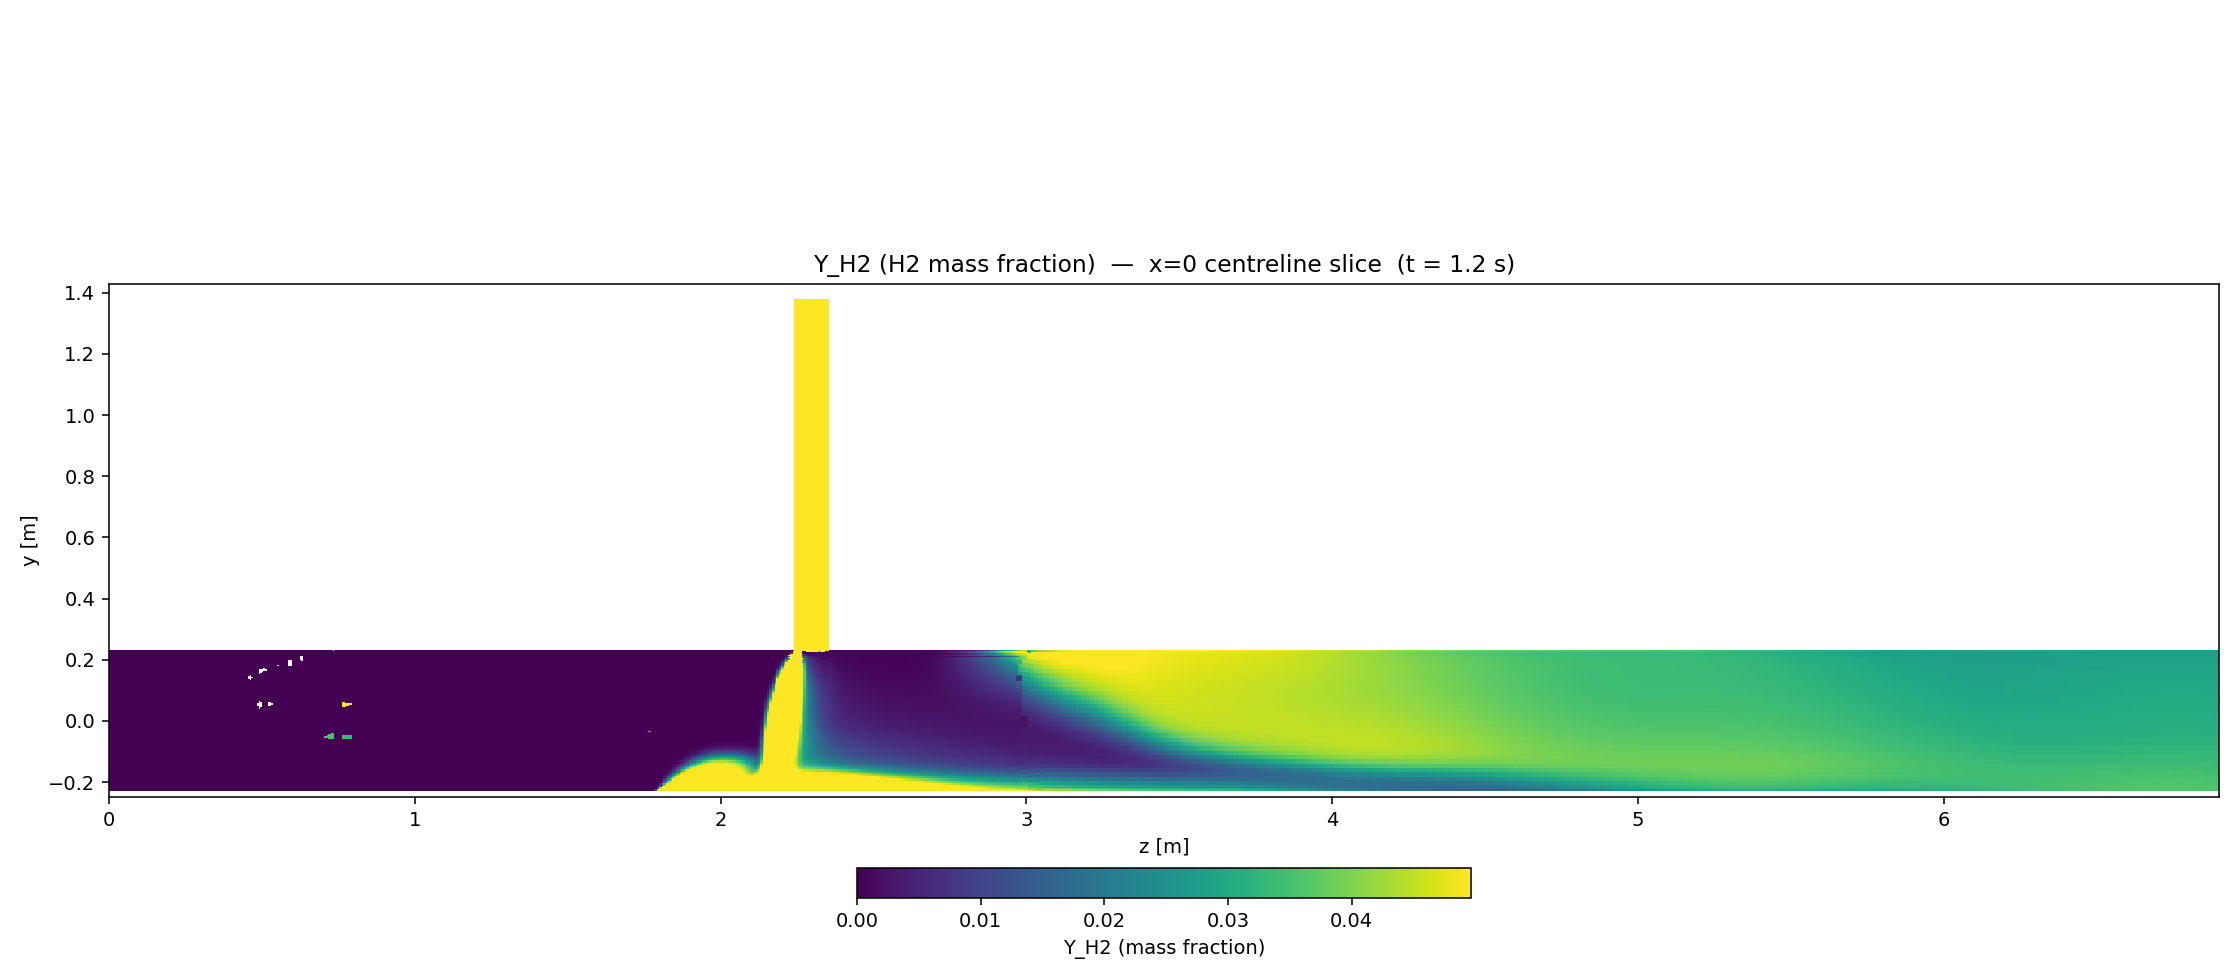
\includegraphics[width=0.78\textwidth]{../doe/results_full/cases/case_04/figures/fig_H2_xz.png}
    \caption{Best-mixing \(90^\circ\) case (case~04,
    \(\dD=0.252\), \(\VR=3.81\), \(\CoV=0.066\)). The jet
    penetrates past the centreline and produces a uniform exit.}
    \label{fig:case04_xz}
\end{figure}

The contrast with case~08 is dramatic (Fig.~\ref{fig:case08_xz}).
The branch is large (\(\dD=0.38\)) but the velocity ratio is
sub-unity, so hydrogen flows out barely faster than the main pipe
sweeps past; the jet bends immediately, attaches to the top wall,
and a hydrogen-rich layer persists to the outlet.

\begin{figure}[H]
    \centering
    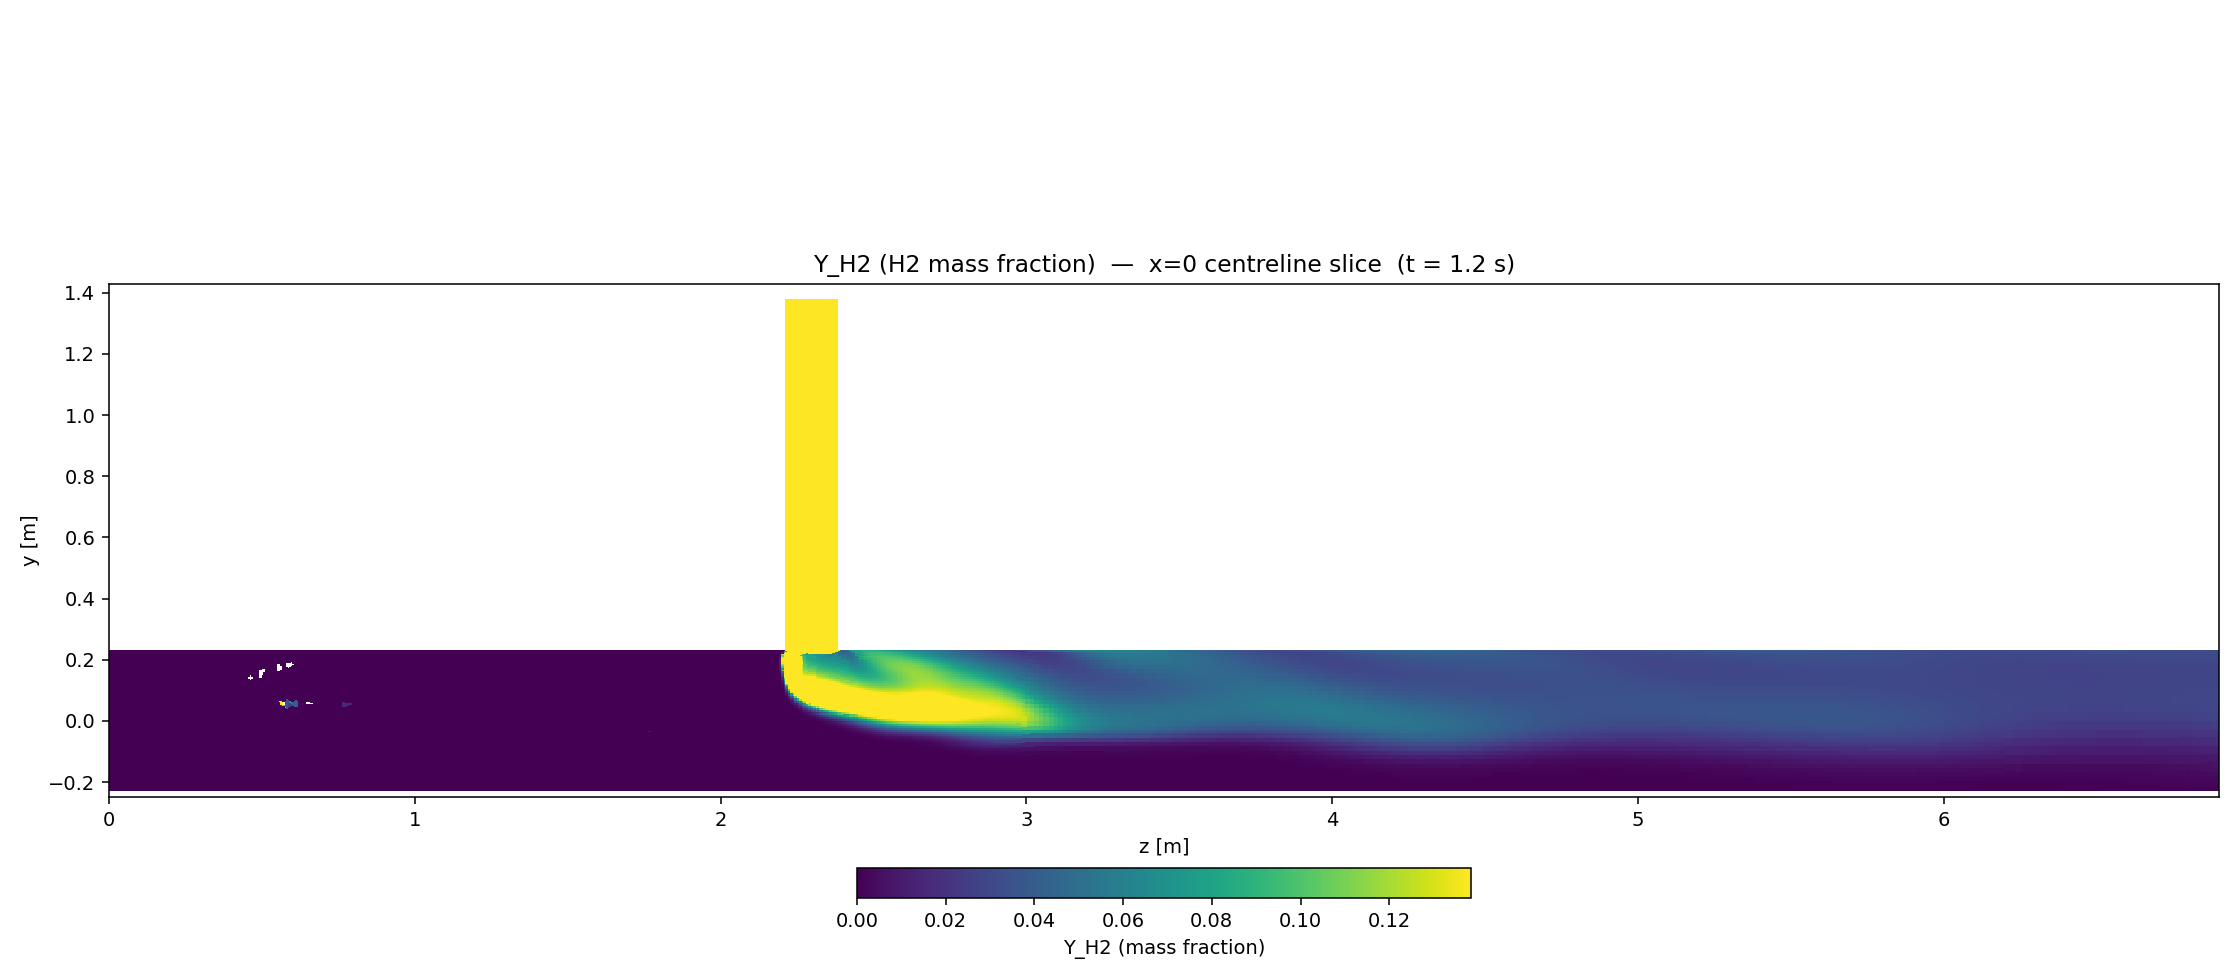
\includegraphics[width=0.78\textwidth]{../doe/results_full/cases/case_08/figures/fig_H2_xz.png}
    \caption{Worst-mixing \(90^\circ\) case (case~08,
    \(\dD=0.38\), \(\VR=0.69\), \(\CoV=0.707\)). The jet attaches
    to the top wall and stratifies.}
    \label{fig:case08_xz}
\end{figure}

\subsection{CoV vs downstream distance}
The spatial evolution of mixing is shown in
Fig.~\ref{fig:cov_zD_90}.  Case~04 exhibits a steep monotonic
decay from \(\CoV\approx 0.7\) near the junction to \(0.06\)
at the outlet, approaching the \(\CoV=0.05\) threshold.
Case~08 decays much more slowly, remaining above \(0.4\) at the
outlet due to persistent crown-layer stratification.

\begin{figure}[H]
    \centering
    \begin{minipage}[t]{0.48\textwidth}
       \centering
       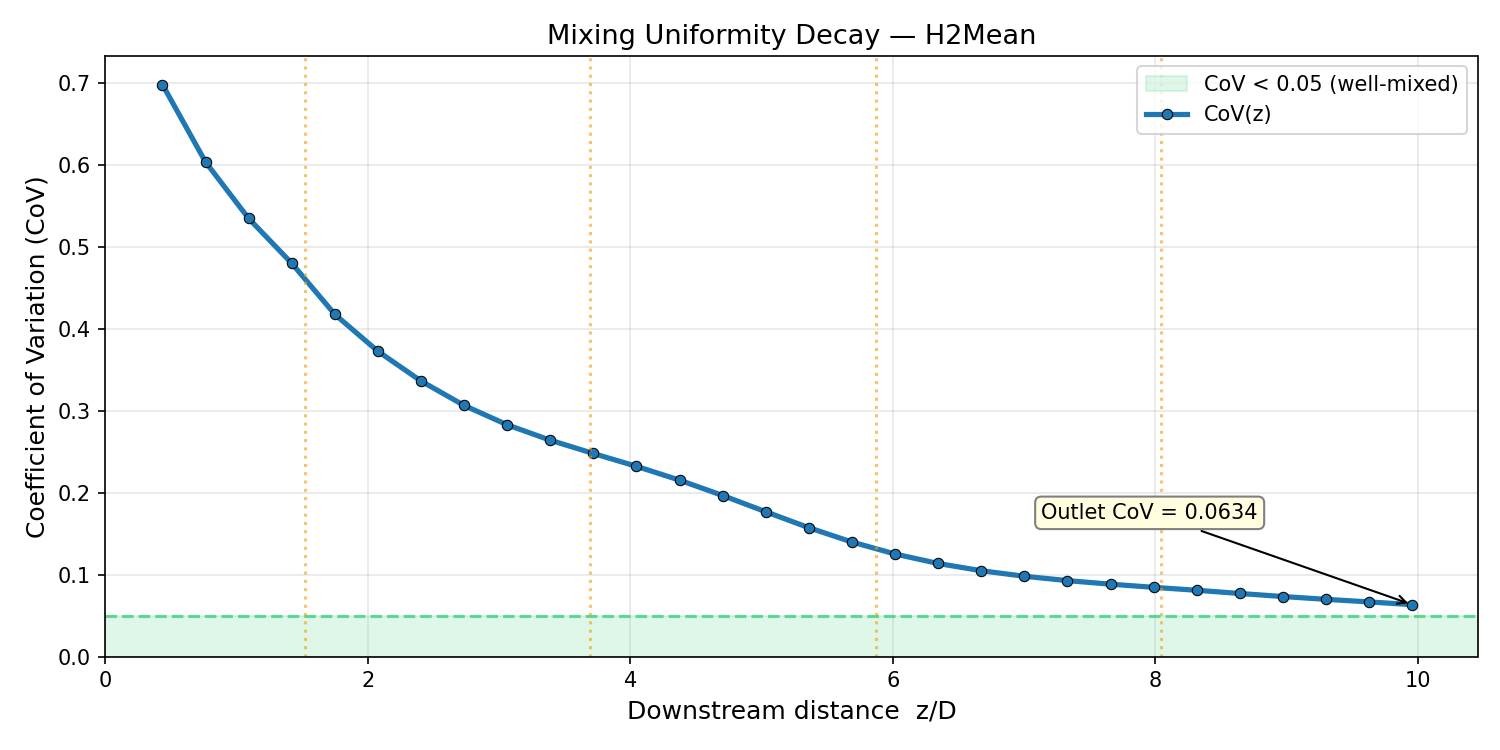
\includegraphics[width=\textwidth]{../doe/results_full/cases/case_04/figures/fig_CoV_vs_zD.png}
    \end{minipage}\hfill
    \begin{minipage}[t]{0.48\textwidth}
       \centering
       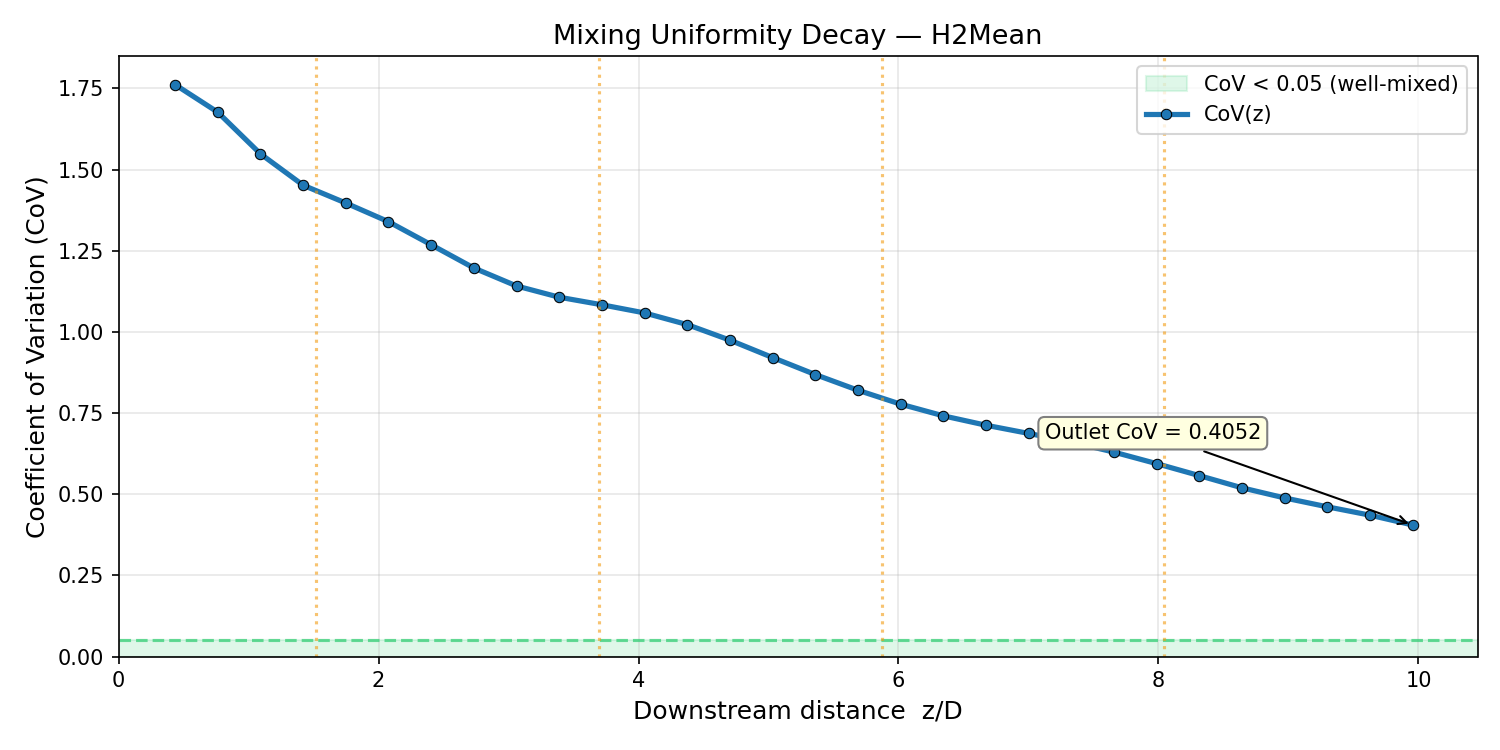
\includegraphics[width=\textwidth]{../doe/results_full/cases/case_08/figures/fig_CoV_vs_zD.png}
    \end{minipage}
    \caption{\CoV{} vs.\ \(z/D\) for case~04 (left) and case~08
    (right).  Green band: \(\CoV<0.05\).}
    \label{fig:cov_zD_90}
\end{figure}

\subsection{Effect of diameter ratio and pressure-drop scaling}
At fixed \HBR{} the influence of \(\dD\) on mixing is weak in
this parameter range; the clear signal is that the \emph{velocity
ratio} dominates mixing, while the \(\dD\) effect reported by
\citet{su2022prediction} is not separable from \(\VR\) variation
in our LHS.
After LP filtering, \(|\Delta p|\) ranges from
\(\SI{1.2}{\kilo\pascal}\) to \(\SI{3.3}{\kilo\pascal}\),
corresponding to a junction loss coefficient
\(K\in[0.5,\,1.4]\), inside the handbook range for an unshaped
diverging tee \citep{idelchik1986handbook}.

% =====================================================================
%  6. RESULTS: 30 deg  (condensed)
% =====================================================================
\section{\texorpdfstring{Results: $30^\circ$ campaign}{Results: 30 deg campaign}}
\label{sec:results_30}

\subsection{Angle-agnostic codebase}
Generalising the \(90^\circ\) pipeline required four changes:
(i)~\texttt{generateSTL.py} reads \texttt{ALPHA\_DEG} and
recomputes the intersection curve analytically;
(ii)~the branch-inlet boundary condition uses a tilted velocity
vector \((0,-\sin\alpha,+\cos\alpha)\,u(r)\);
(iii)~\texttt{stamp\_cases.py} substitutes angle tokens;
(iv)~\texttt{snappyHexMeshDict}'s seed point is placed inside the
tilted branch volume.

\subsection{Mesh defect and fix}
\label{sec:30deg_meshfix}
The first \(30^\circ\) launch produced two disconnected fluid
regions (\(462\,\mathrm{k}\) cells in the main pipe,
\(22\,\mathrm{k}\) in the branch).
The root cause was the zipper-hole heuristic in
\texttt{generateSTL.py}, which at \(\alpha=30^\circ\) sized the
rectangular hole \(7\times\) wider than the actual intersection,
producing distorted triangles that \texttt{snappyHexMesh}
interpreted as an internal wall.
The fix replaces the heuristic with a tight bounding box on the
intersection points, padded by two grid cells; it is
angle-agnostic and leaves the \(90^\circ\) mesh unchanged.

\subsection{DoE summary}
Nine of ten cases completed (Table~\ref{tab:30deg_summary});
case~04 stopped at \(t=\SI{0.215}{\second}\) (wall-time limit)
and is excluded.
Case~01 achieves \(\CoV=0.005\), an order of magnitude below the
industrial target.  At sub-unity \VR{} (cases~08--10) the
campaign sits on a plateau of \(\CoV\approx 0.30\)-\(0.35\).

\begin{table}[H]
\centering\scriptsize
\caption{\(30^\circ\) campaign summary (case~04 incomplete, omitted).}
\label{tab:30deg_summary}
\begin{tabular}{ccccrr}
\toprule
case & \(\dD\) & \(\VR\) & \(\HBR\) & \CoV{} & \(|\Delta p|\) (kPa) \\
\midrule
01 & 0.196 & 5.842 & 0.184 & \textbf{0.005} & 4.2 \\
02 & 0.196 & 1.643 & 0.060 & 0.390 & 0.6 \\
03 & 0.252 & 1.330 & 0.078 & 0.278 & 0.5 \\
05 & 0.296 & 1.241 & 0.098 & 0.298 & 0.6 \\
06 & 0.296 & 2.614 & 0.187 & 0.088 & 1.3 \\
07 & 0.382 & 1.137 & 0.142 & 0.238 & 0.8 \\
08 & 0.382 & 0.693 & 0.092 & 0.327 & 0.6 \\
09 & 0.396 & 0.953 & 0.130 & 0.307 & 0.3 \\
10 & 0.396 & 0.806 & 0.112 & 0.345 & 0.5 \\
\bottomrule
\end{tabular}
\end{table}

\begin{figure}[H]
    \centering
    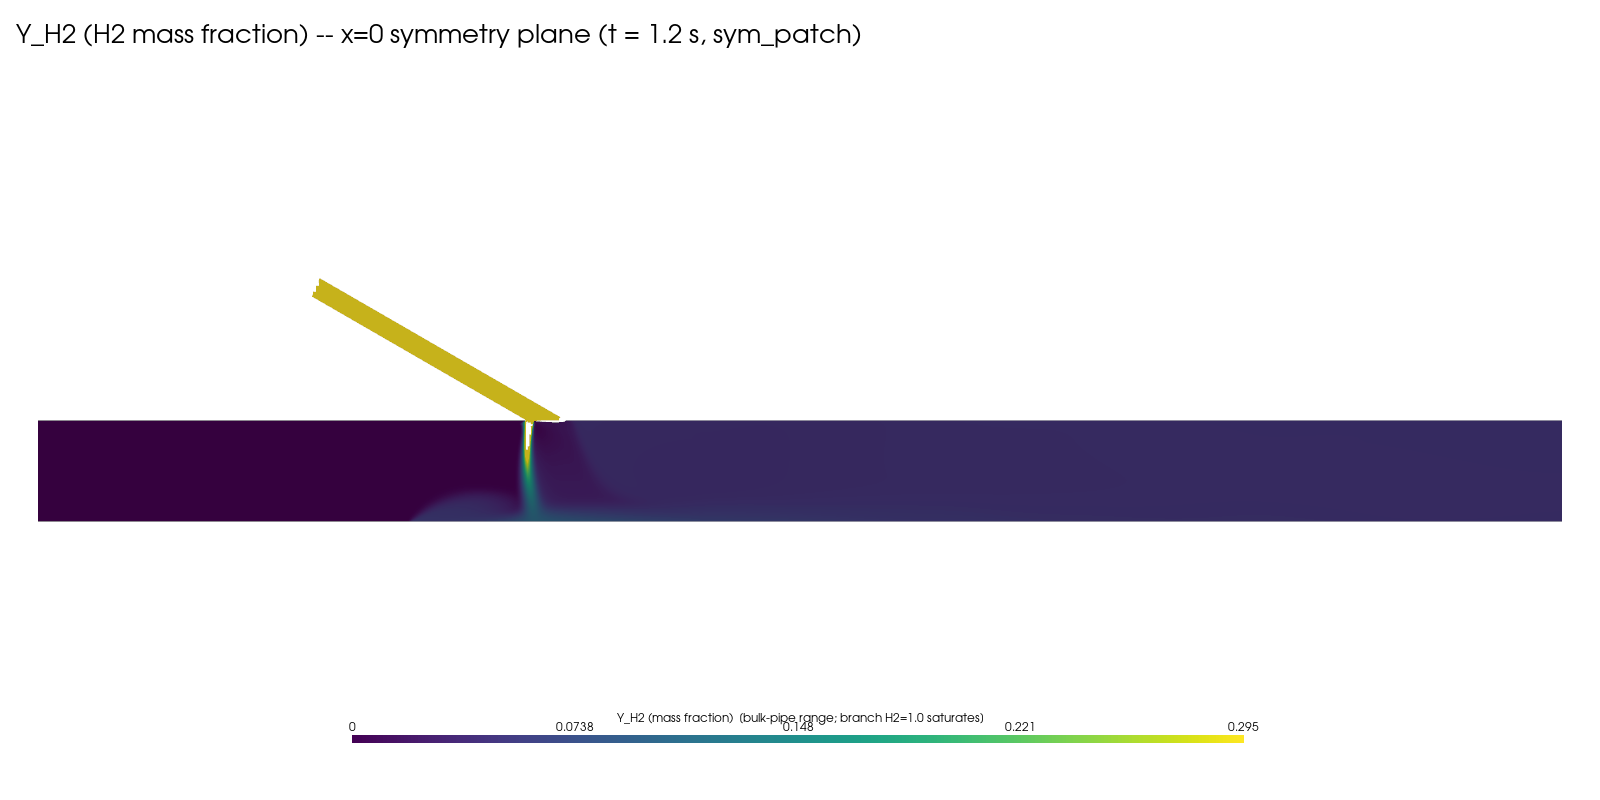
\includegraphics[width=0.78\textwidth]{../doe/results_full_30deg/cases/case_01/figures/fig_H2_xz.png}
    \caption{Best-mixing \(30^\circ\) case (case~01,
    \(\VR=5.84\), \(\CoV=0.005\)). The plume fills the
    cross-section by \(z\approx 3\,\si{\meter}\).}
    \label{fig:case01_30_xz}
\end{figure}

\begin{figure}[H]
    \centering
    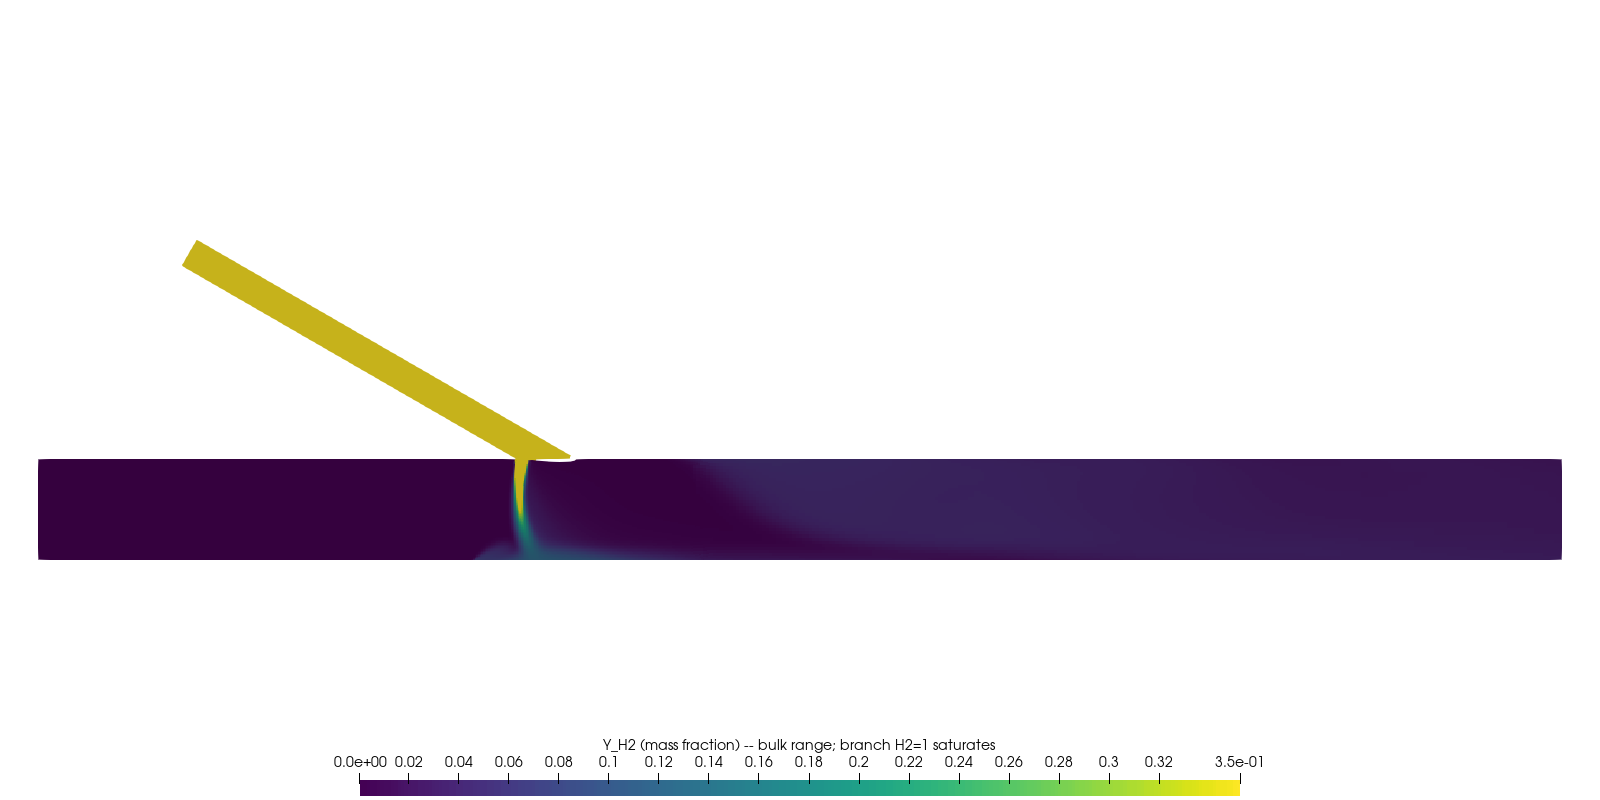
\includegraphics[width=0.78\textwidth]{../doe/results_full_30deg/cases/case_06/figures/fig_H2_xz.png}
    \caption{Intermediate \(30^\circ\) case (case~06,
    \(\VR=2.61\), \(\CoV=0.088\)). A wavy lower edge indicates
    a strong streamwise vortex pair.}
    \label{fig:case06_30_xz}
\end{figure}

\begin{figure}[H]
    \centering
    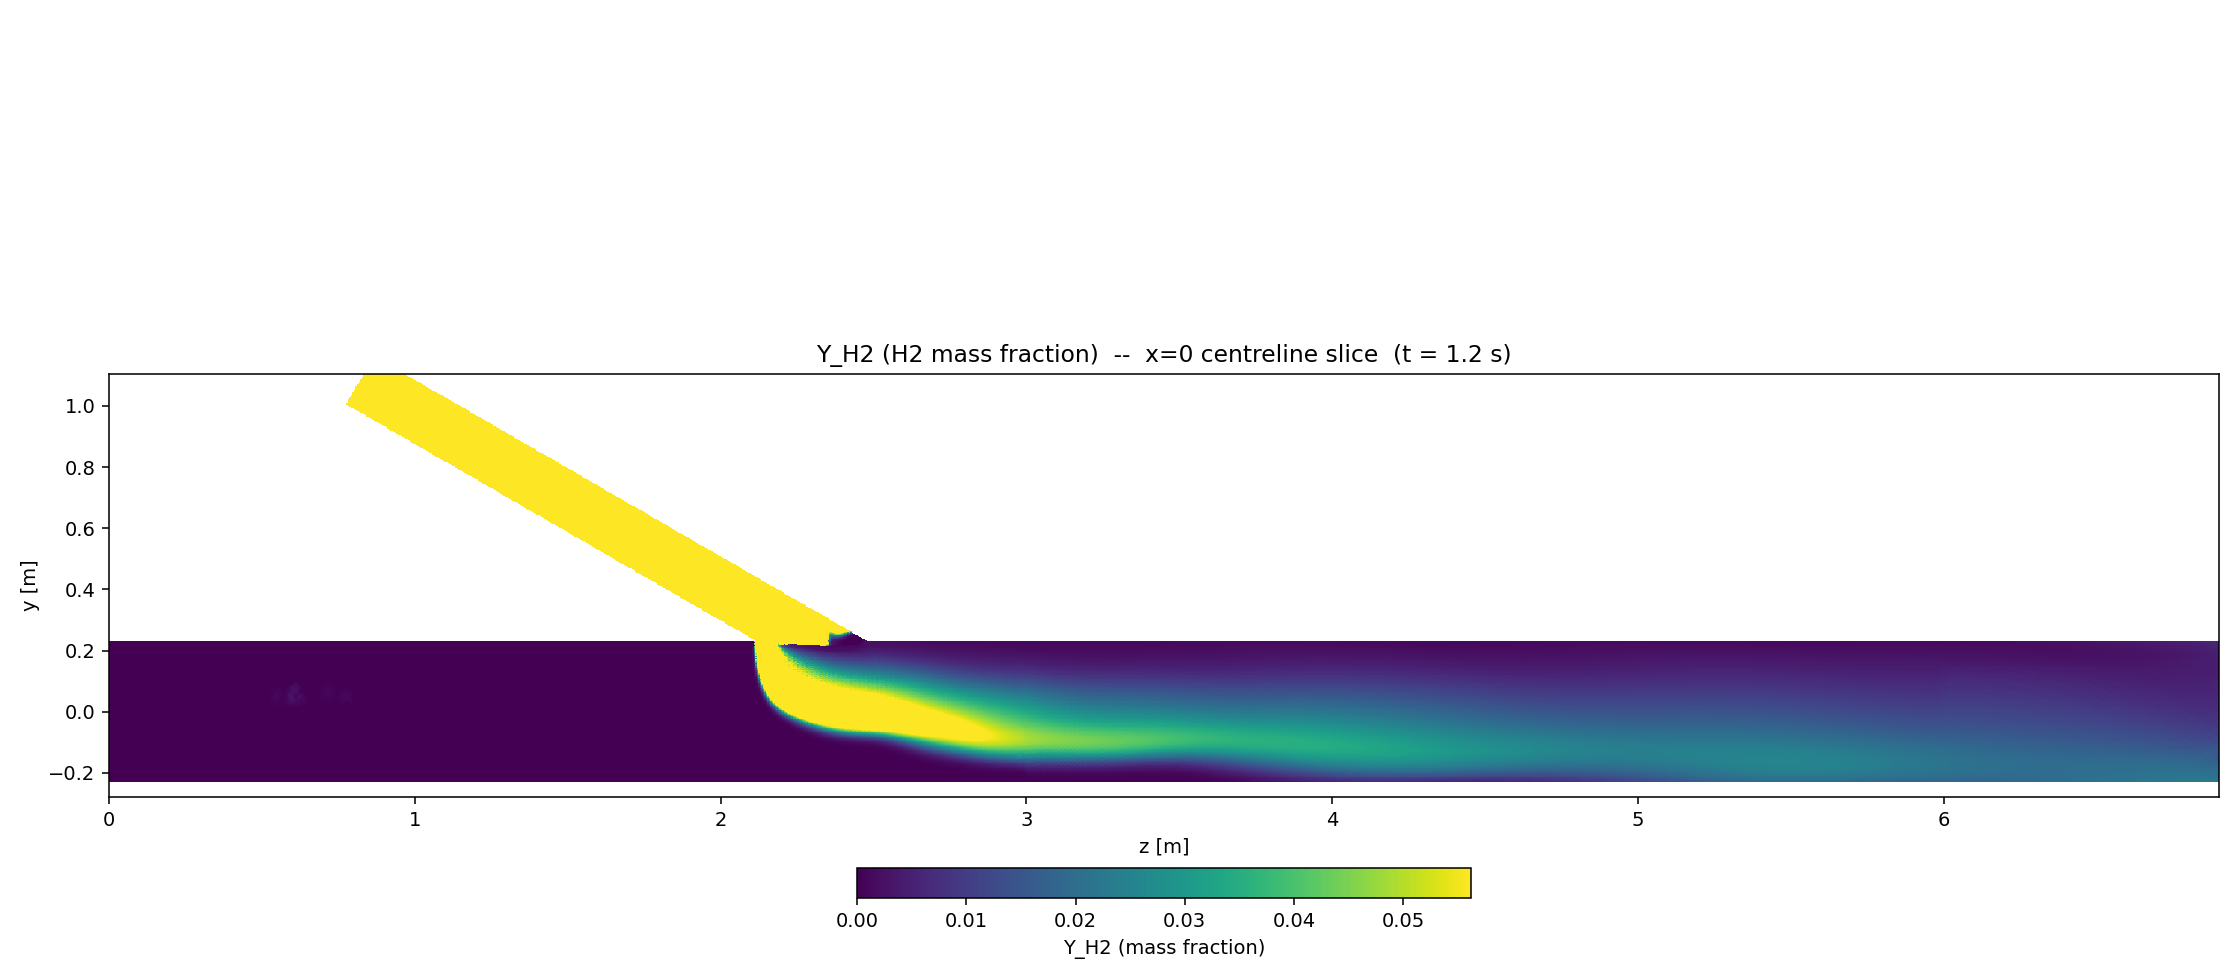
\includegraphics[width=0.78\textwidth]{../doe/results_full_30deg/cases/case_10/figures/fig_H2_xz.png}
    \caption{Worst-mixing \(30^\circ\) case (case~10,
    \(\VR=0.81\), \(\CoV=0.345\)). The jet attaches to the top
    wall, similar to the \(90^\circ\) mechanism.}
    \label{fig:case10_30_xz}
\end{figure}

% =====================================================================
%  7. CROSS-CAMPAIGN: ANGLE EFFECT
% =====================================================================
\section{Cross-campaign synthesis: angle effect}
\label{sec:cross}

Seven case IDs (3, 5, 6, 7, 8, 9, 10) share the same
\((\dD,\VR)\) across both angles.

\subsection{Matched-pair finding}
\label{sec:cross_pairs}
Table~\ref{tab:matched} and Fig.~\ref{fig:paired_comparison} show
the comparison.  The \(30^\circ\) tilt reduces \CoV{} in
\textbf{all seven} pairs (median \(-46\,\%\), range
\(15\)-\(56\,\%\)) and \(|\Delta p|\) in \textbf{all seven}
(median \(-63\,\%\), range \(56\)-\(86\,\%\)).
The matched-pair \(|\Delta p|\) differences range from
\(-0.7\,\si{\kilo\pascal}\) to \(-1.7\,\si{\kilo\pascal}\);
with \(\pm\SI{0.5}{\kilo\pascal}\) per-case uncertainty the
pair-difference uncertainty is
\(\sigma_{\Delta}\approx\SI{0.7}{\kilo\pascal}\).
Under the null hypothesis, the probability of all seven signs
agreeing is \(2^{1-7}=1.6\,\%\).
The tilt therefore simultaneously improves mixing \emph{and}
lowers pumping cost.

\begin{table}[H]
\centering\scriptsize
\caption{Matched-pair angle effect.}
\label{tab:matched}
\begin{tabular}{cccc rr r rr r}
\toprule
case & \(\dD\) & \(\VR\) & \(\HBR\) &
\(\CoV_{90}\) & \(\CoV_{30}\) & \(\Delta\CoV\) &
\(|\Delta p|_{90}\) & \(|\Delta p|_{30}\) & \(\Delta|\Delta p|\) \\
& & & & & & (\%) & (kPa) & (kPa) & (\%) \\
\midrule
03 & 0.252 & 1.33 & 0.078 & 0.472 & 0.278 & \(-41\) & 1.2 & 0.5 & \(-56\) \\
05 & 0.296 & 1.24 & 0.098 & 0.577 & 0.298 & \(-48\) & 1.6 & 0.6 & \(-63\) \\
06 & 0.296 & 2.61 & 0.187 & 0.202 & 0.088 & \(-56\) & 3.1 & 1.3 & \(-57\) \\
07 & 0.382 & 1.14 & 0.142 & 0.440 & 0.238 & \(-46\) & 2.2 & 0.8 & \(-63\) \\
08 & 0.382 & 0.69 & 0.092 & 0.707 & 0.327 & \(-54\) & 1.3 & 0.6 & \(-58\) \\
09 & 0.396 & 0.95 & 0.130 & 0.390 & 0.307 & \(-21\) & 2.0 & 0.3 & \(-86\) \\
10 & 0.396 & 0.81 & 0.112 & 0.407 & 0.345 & \(-15\) & 1.5 & 0.5 & \(-66\) \\
\bottomrule
\end{tabular}
\end{table}

\begin{figure}[H]
    \centering
    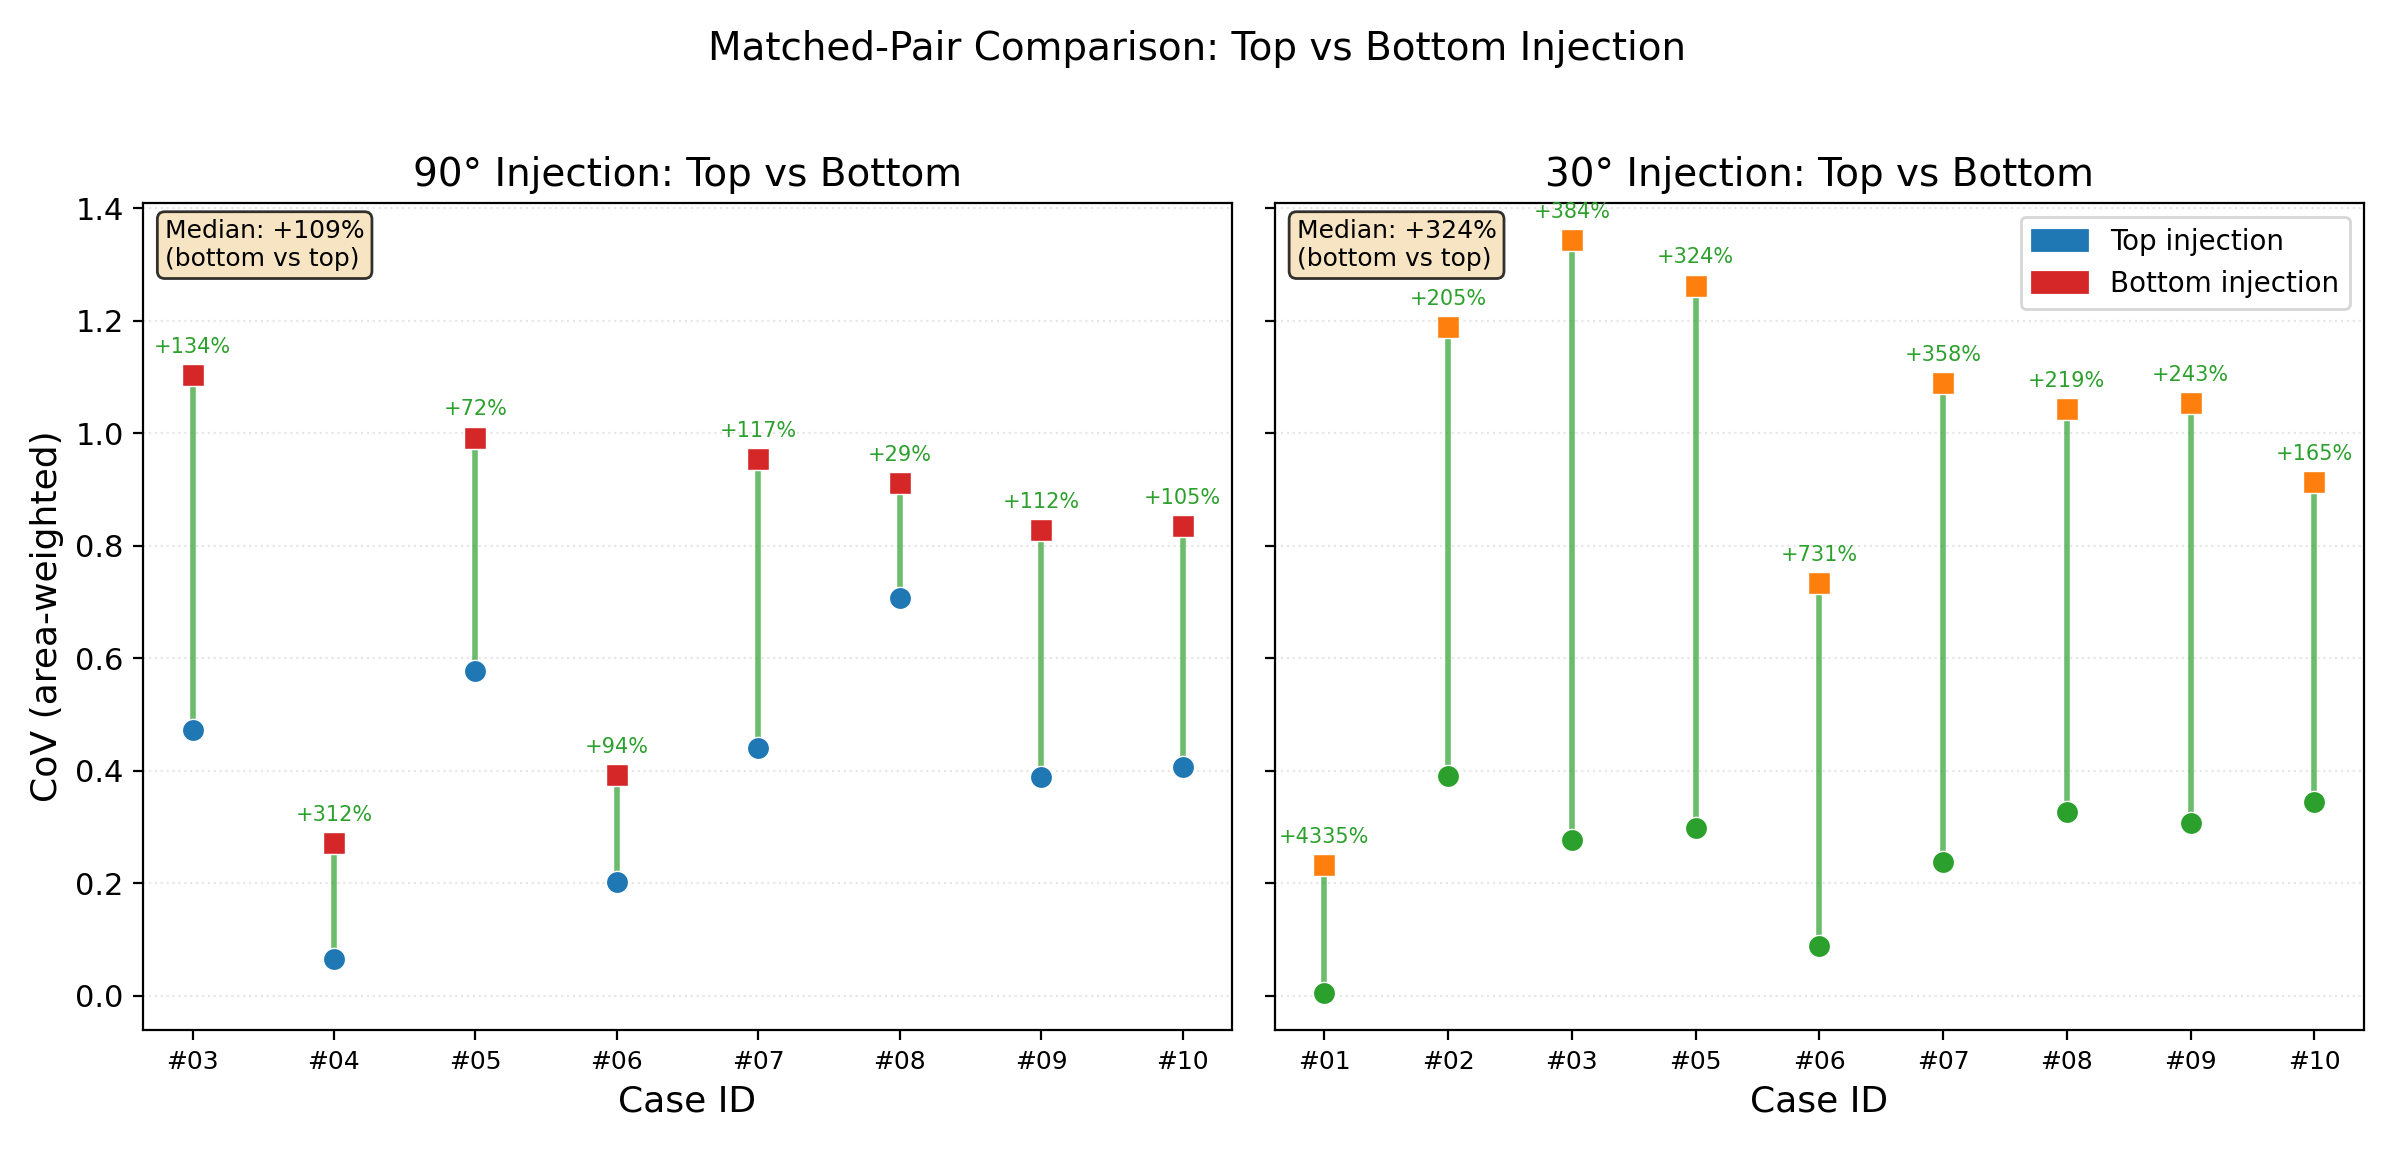
\includegraphics[width=0.85\textwidth]{../doe/cross_campaign/figures/fig2_matched_pairs_top_vs_bottom.png}
    \caption{Matched-pair arrow plot: every arrow points toward
    the \(30^\circ\) case, showing simultaneous improvement in
    both \CoV{} and \(|\Delta p|\).}
    \label{fig:paired_comparison}
\end{figure}

\subsection{Power-law scaling}
\label{sec:cross_scaling}
A log-log fit gives
\(\CoV \approx 0.475\,\VR^{-1.16}\) at \(90^\circ\)
(\(R^2=0.80\)) and
\(\CoV \approx 0.334\,\VR^{-1.88}\) at \(30^\circ\)
(\(R^2=0.80\)).
Each unit of \(\VR\) buys nearly twice the mixing improvement on
the tilted geometry (Fig.~\ref{fig:powerlaw}).

\begin{figure}[H]
    \centering
    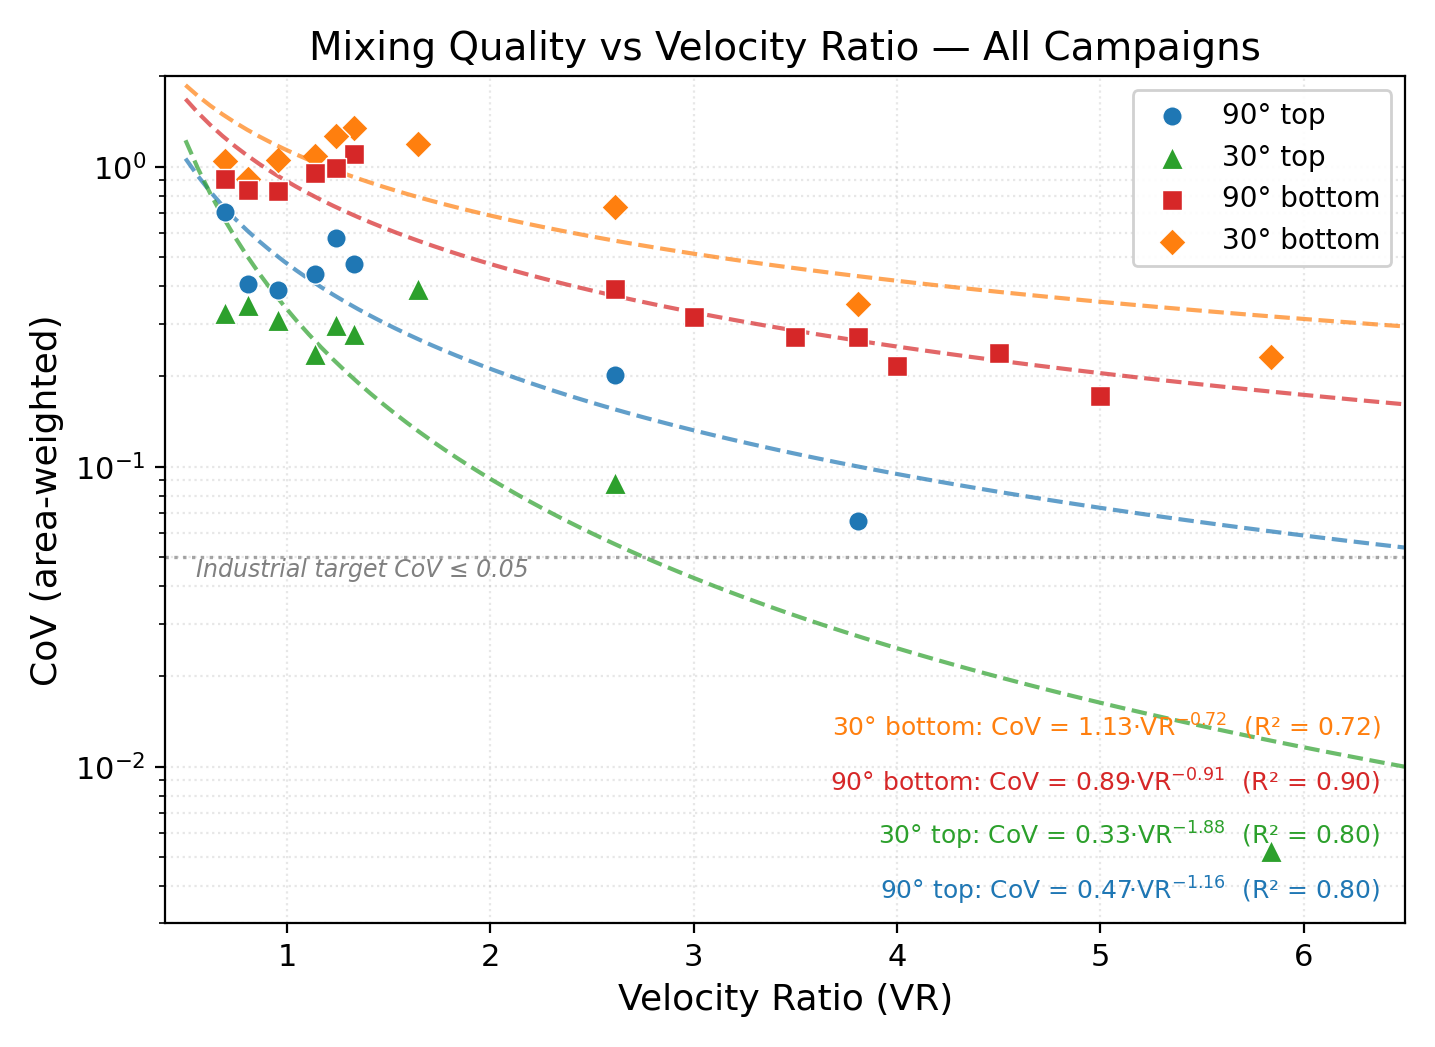
\includegraphics[width=0.75\textwidth]{../doe/cross_campaign/figures/fig1_CoV_vs_VR.png}
    \caption{Power-law fit of \CoV{} vs.\ \VR.
    The dashed line marks \(\CoV=0.05\).}
    \label{fig:powerlaw}
\end{figure}

\subsection{Pareto front}
\label{sec:cross_pareto}
The combined Pareto plot (Fig.~\ref{fig:pareto}) shows that every
\(90^\circ\) point is dominated by a \(30^\circ\) point.
Case~01 of the \(30^\circ\) campaign reaches \(\CoV=0.5\,\%\) at
\(|\Delta p|\approx\SI{4.2}{\kilo\pascal}\).

\begin{figure}[H]
    \centering
    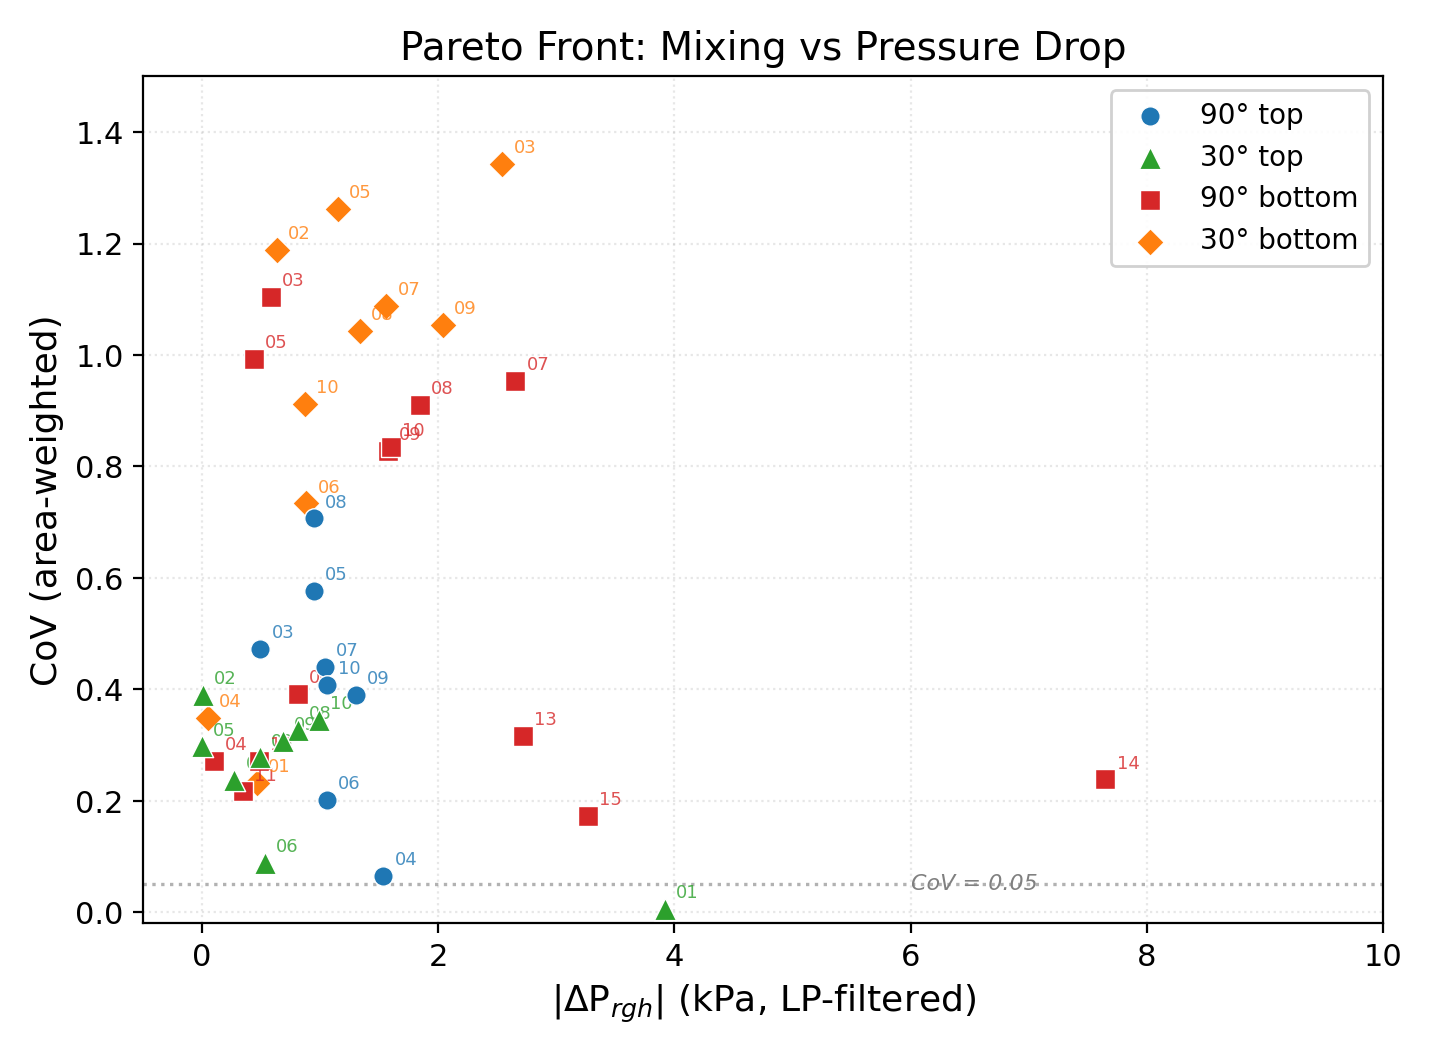
\includegraphics[width=0.75\textwidth]{../doe/cross_campaign/figures/fig3_pareto.png}
    \caption{Pareto front: \CoV{} vs.\ \(|\Delta p|\).
    Lower-left is better.}
    \label{fig:pareto}
\end{figure}

\subsection{Physical mechanism: why does the tilt help?}
\label{sec:cross_mech}
A side-by-side view (Fig.~\ref{fig:xz_montage}) makes the
mechanism visible.  Two effects are at play:
\begin{enumerate}
    \item The perpendicular jet impinges on the opposite wall,
    splits laterally and traps a low-\Hi{} core under the
    junction; hydrogen escapes only by slow diffusion.
    The tilted jet lays its momentum into a streamwise shear
    layer resolved by SST as high-\(k\), which entrains methane.
    \item The recirculation under the tilted junction is longer
    in \(z\), so the residence time for mixing is larger.
\end{enumerate}
The net effect: more of the pipe length does useful mixing, and
the junction \(|\Delta p|\) is smaller because the branch
momentum is partially aligned with the main flow.
The loss coefficient
\(K=|\Delta p|/q_{\mathrm{dyn,main}}\) lands at
median \(K_{90^\circ}\!\approx 0.78\) and
\(K_{30^\circ}\!\approx 0.26\), consistent with
\citet{idelchik1986handbook}.

\begin{figure}[H]
    \centering
    \begin{subfigure}[b]{0.48\textwidth}
       \centering
       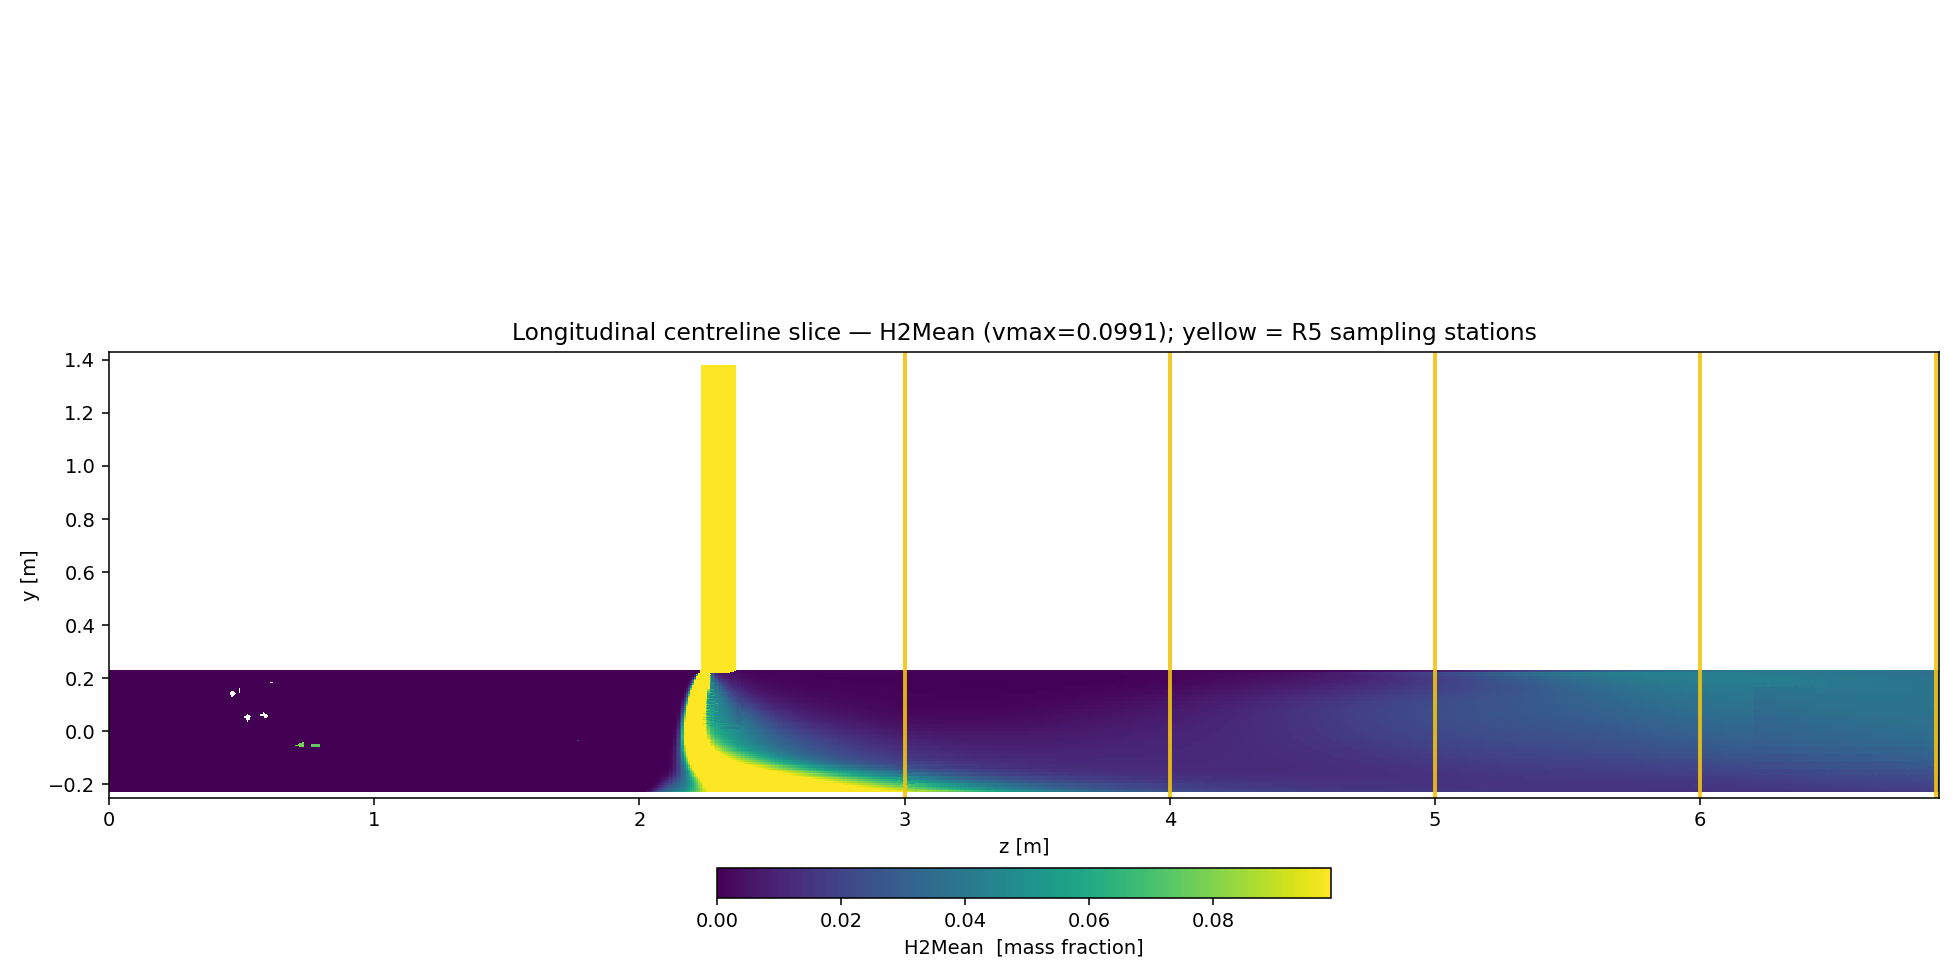
\includegraphics[width=\textwidth]{../doe/results_full/cases/case_06/figures/fig_H2_long.png}
       \caption{\(90^\circ\), case~06 (\(\CoV=0.20\))}
    \end{subfigure}\hfill
    \begin{subfigure}[b]{0.48\textwidth}
       \centering
       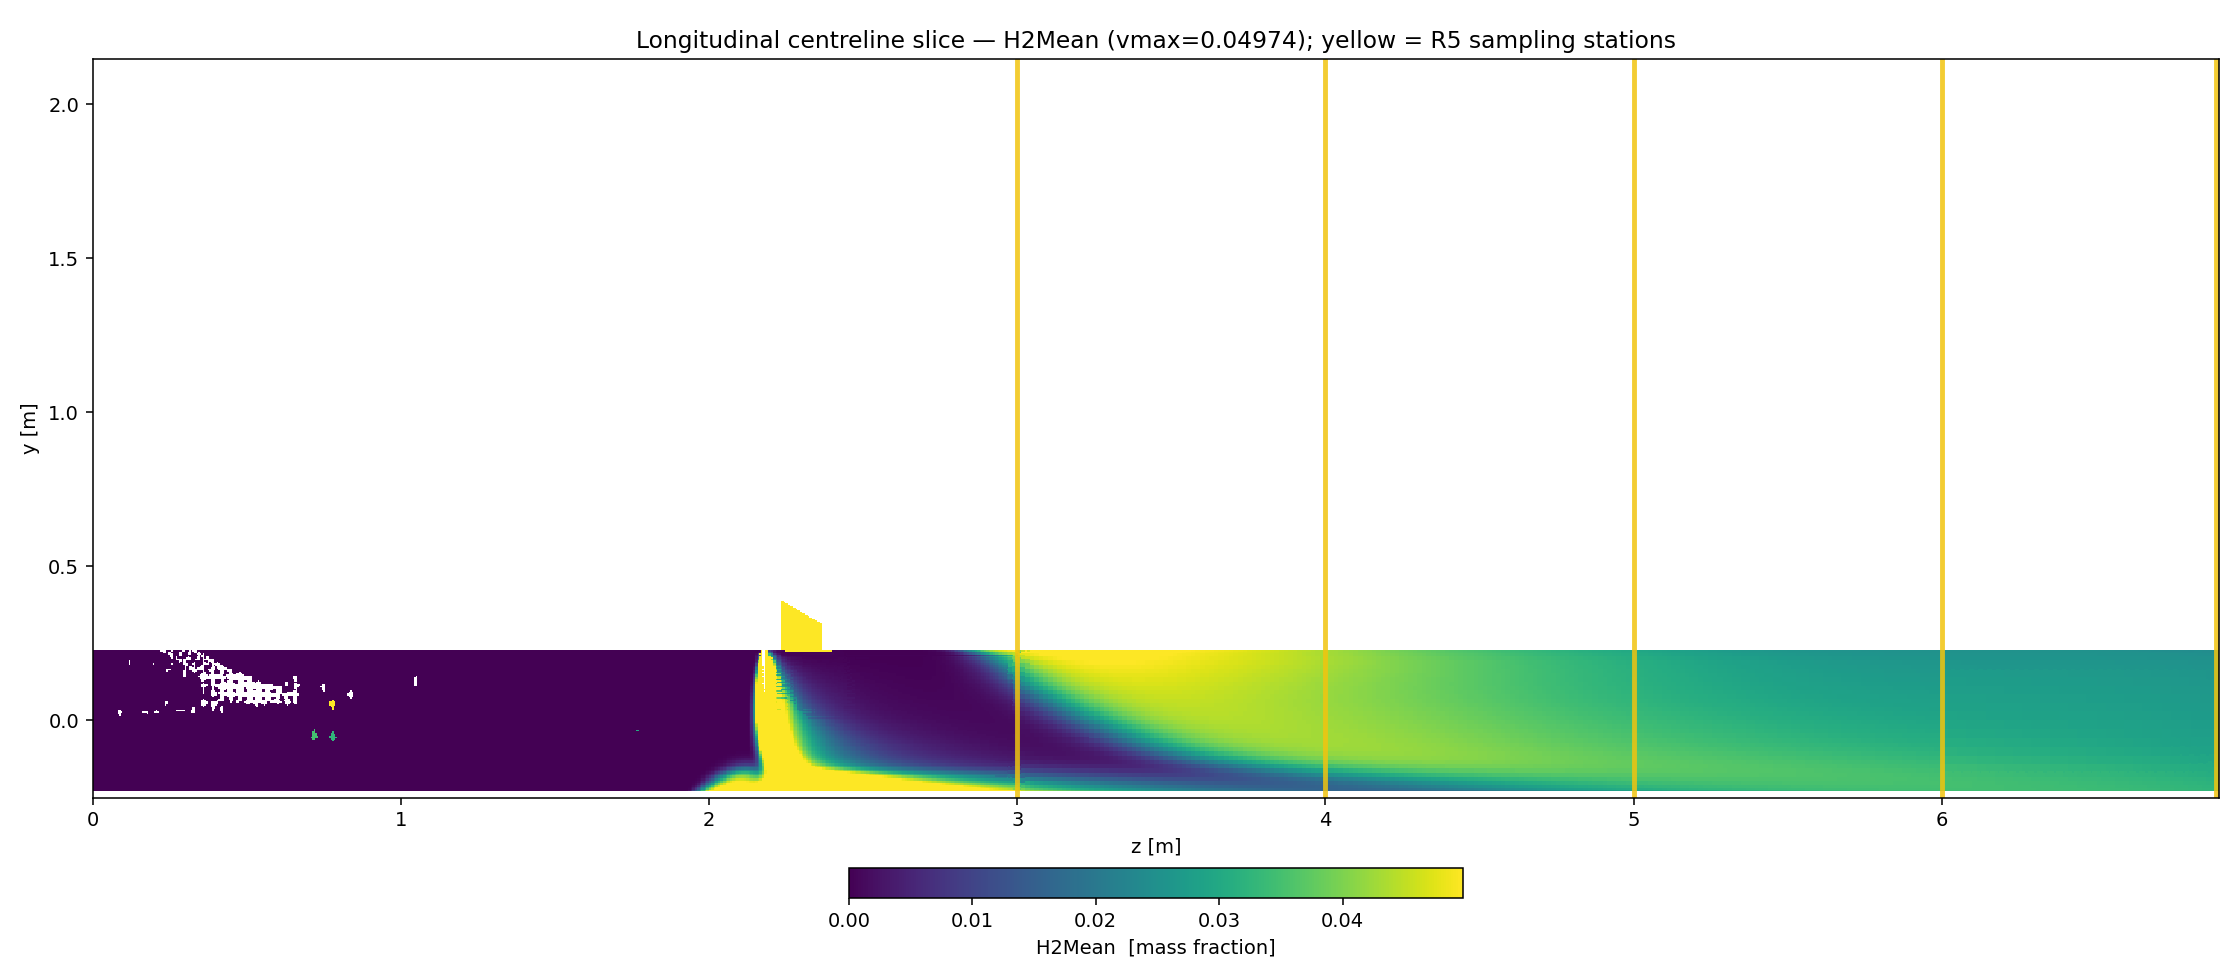
\includegraphics[width=\textwidth]{../doe/results_full_30deg/cases/case_06/figures/fig_H2_long.png}
       \caption{\(30^\circ\), case~06 (\(\CoV=0.09\))}
    \end{subfigure}
    \caption{Longitudinal \(Y_{\Hi}\) for a matched pair (case~06,
    \(\dD=0.296\), \(\VR=2.61\)).}
    \label{fig:xz_montage}
\end{figure}

% =====================================================================
%  8. BOTTOM INJECTION  (condensed)
% =====================================================================
\section{Results: bottom injection}
\label{sec:bottom}

Two additional campaigns relocated the branch to the bottom of the
pipe (\(y=-R_1\)): 13~valid cases at \(90^\circ\) (including
5~supplementary high-\VR{} cases) and 10 at \(30^\circ\)
(Table~\ref{tab:bot_summary}).

\begin{table}[H]
\centering\scriptsize
\caption{Bottom-injection campaign summary.}
\label{tab:bot_summary}
\begin{tabular}{l c c c c}
\toprule
Campaign & Valid & \CoV{} range & \CoV{} median
& \(|\Delta p|\) median (kPa) \\
\midrule
\(90^\circ\) bottom & 13 & 0.17--1.10 & 0.39 & 1.58 \\
\(30^\circ\) bottom & 10 & 0.23--1.34 & 1.05 & 1.02 \\
\bottomrule
\end{tabular}
\end{table}

Figure~\ref{fig:bot_strip_04} compares the cross-sectional
evolution for case~04 (\(\dD=0.252\), \(\VR=3.81\)) --- the
highest-\VR{} matched pair.
With top injection, the high-\VR{} jet punches downward; buoyancy
prevents the lighter \Hi{} from falling further, so the gas
flattens against the upper wall and spreads laterally into a thin,
wide layer with maximum surface area for turbulent diffusion.
By \(z\approx 5\,D\) the cross-section is virtually uniform
(\(\CoV=0.066\)).
With bottom injection, buoyancy \emph{assists} the jet: the plume
rises as a coherent, narrow column that never fans out laterally.
By the outlet the \Hi{} is concentrated in the upper half as a
mushroom-shaped streak (\(\CoV=0.271\), \(4\times\) worse).

\begin{figure}[H]
    \centering
    \begin{subfigure}[b]{\textwidth}
        \centering
        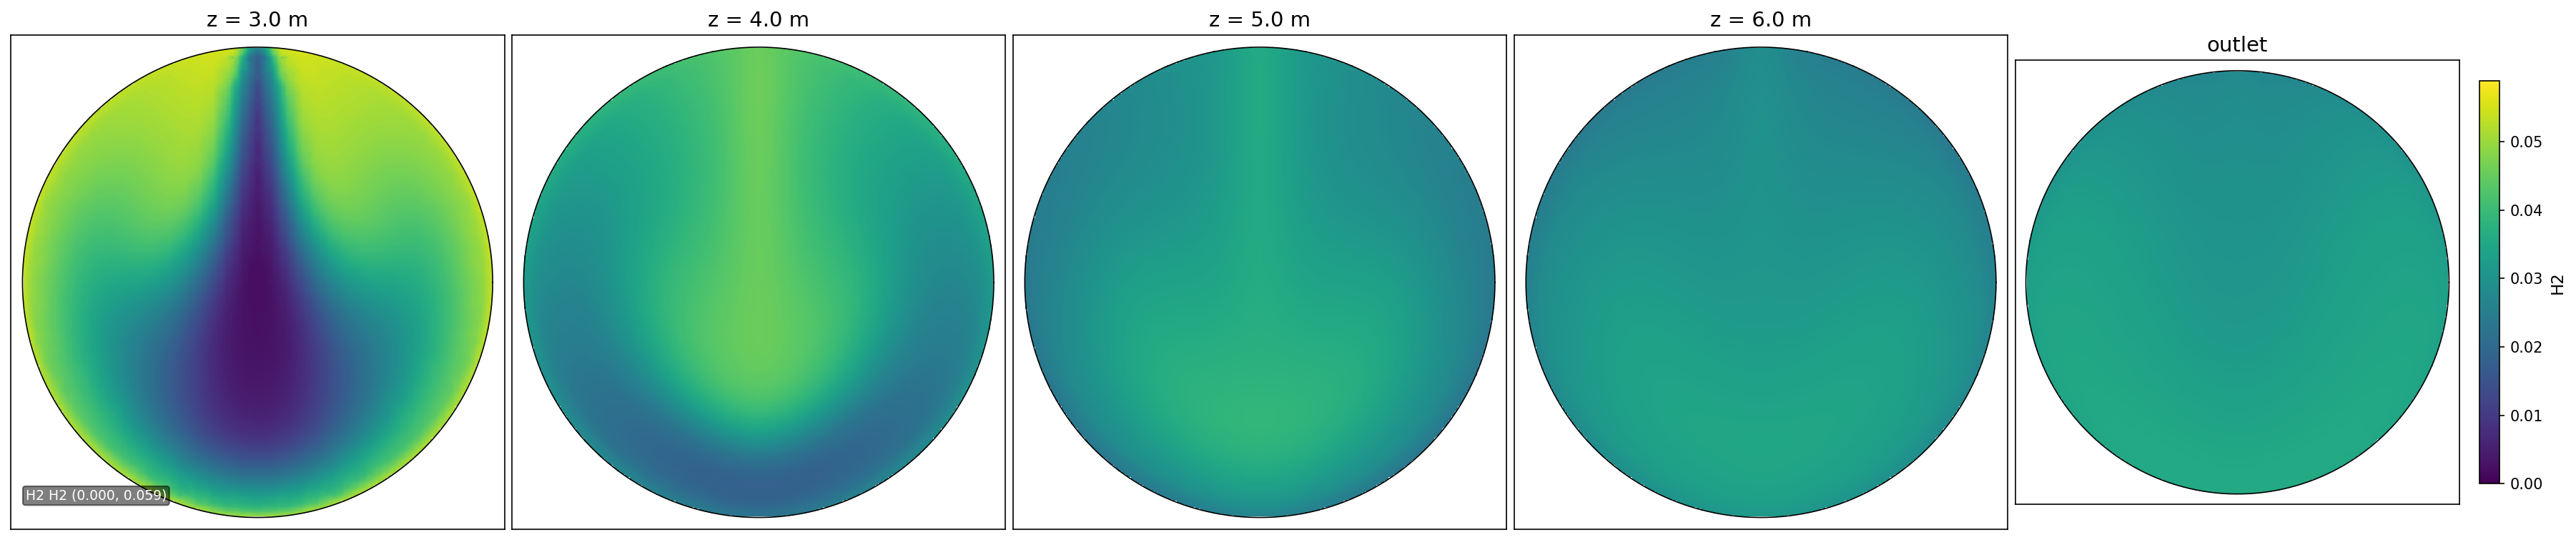
\includegraphics[width=0.85\textwidth]{../doe/results_full/cases/case_04/figures/fig_H2_strip.png}
        \caption{Top injection (\(\CoV = 0.066\)). By \(z=5\,\mathrm{m}\)
        the cross-section is essentially uniform.}
        \label{fig:strip_04_top}
    \end{subfigure}\\[3pt]
    \begin{subfigure}[b]{\textwidth}
        \centering
        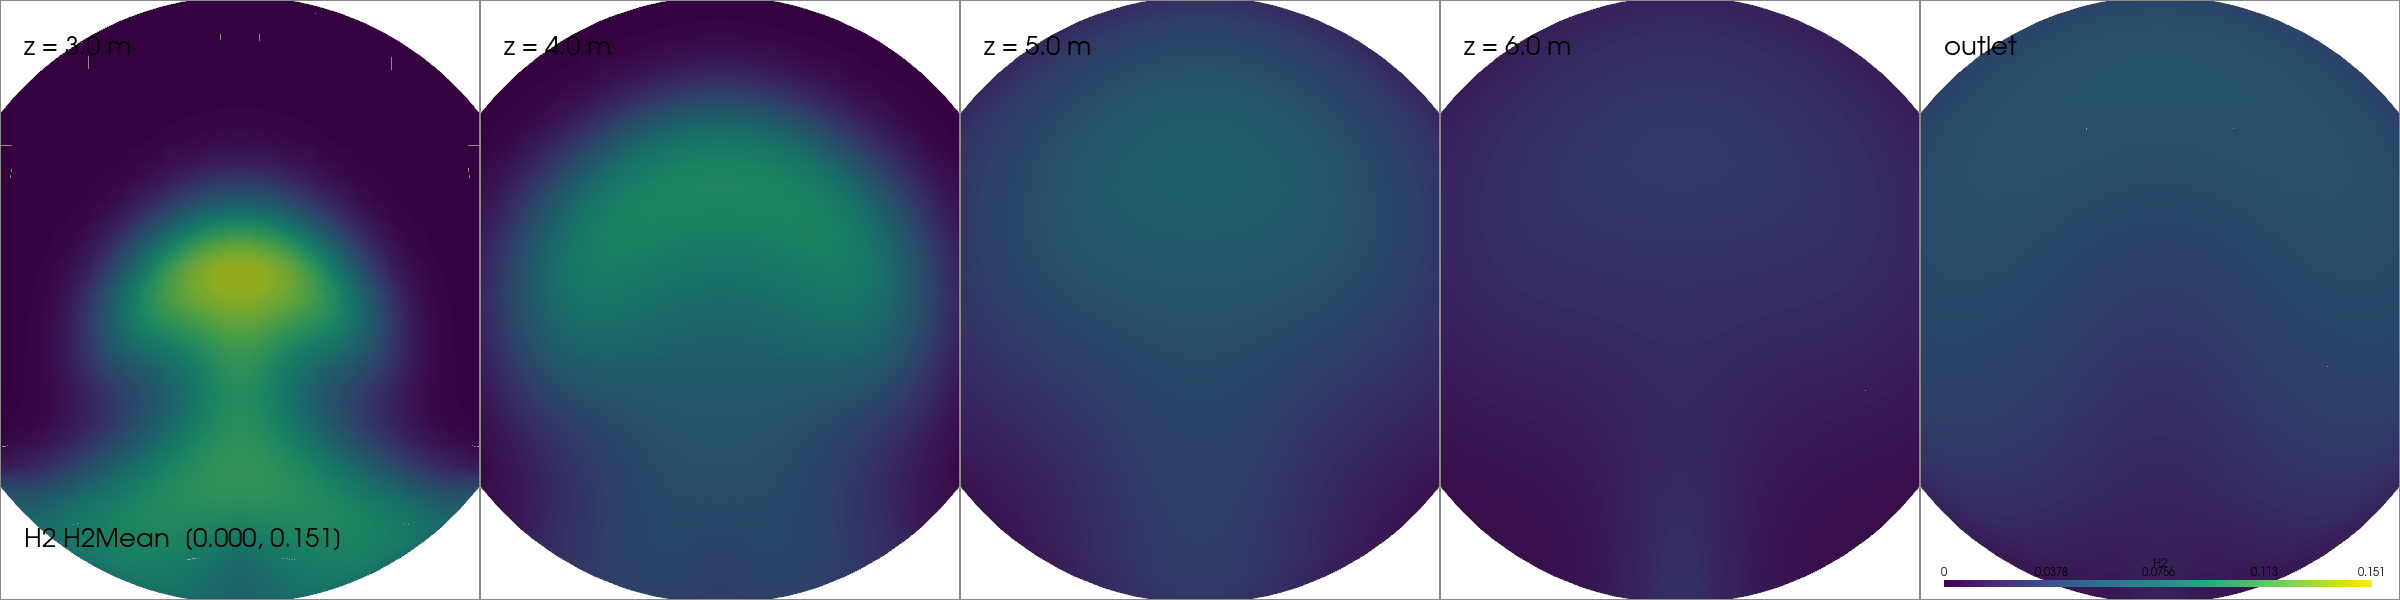
\includegraphics[width=0.85\textwidth]{../doe/results_full_90deg_bottom/case_04/figures/fig_H2_strip.png}
        \caption{Bottom injection (\(\CoV = 0.271\)). The plume is a
        concentrated mushroom in the lower half; the gradient persists
        to the outlet.}
        \label{fig:strip_04_bot}
    \end{subfigure}
    \caption{Cross-sectional H\(_2\) strip for case~04
    (\(\dD=0.252\), \(\VR=3.81\)) at \(90^\circ\): top (a) vs.\
    bottom (b).  Both are time-averaged at \(t=\SI{1.2}{\second}\).}
    \label{fig:bot_strip_04}
\end{figure}

\subsection{Longitudinal centreline comparison}
Figure~\ref{fig:bot_long_04} shows the centreline slice for the
same pair.  With top injection the plume penetrates deep and then
diffuses uniformly; with bottom injection it clings to the bottom
wall and rises slowly --- the bright concentration core extends
several diameters further downstream.

\begin{figure}[H]
    \centering
    \begin{subfigure}[b]{\textwidth}
        \centering
        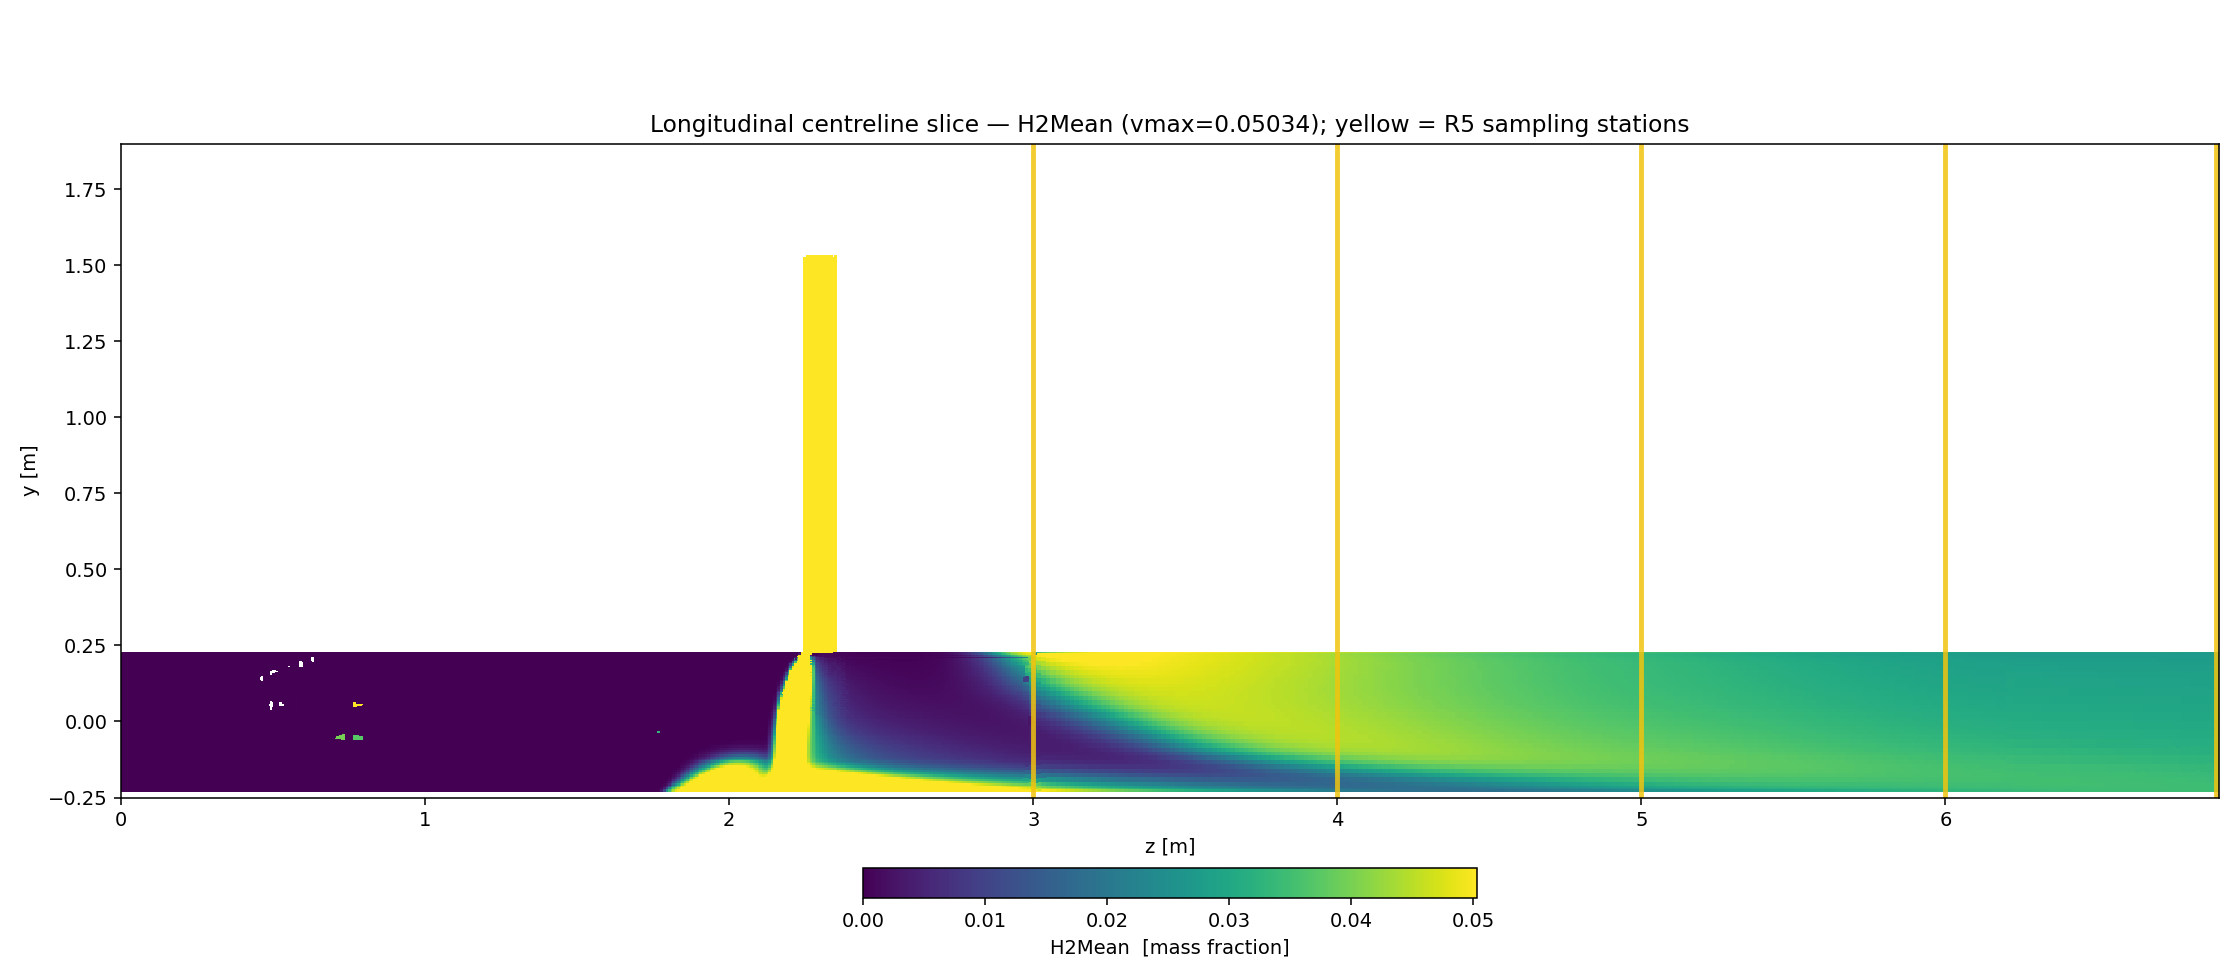
\includegraphics[width=0.85\textwidth]{../doe/results_full/cases/case_04/figures/fig_H2_long.png}
        \caption{Top injection --- \Hi{} fills the pipe by
        \(z\approx 3\,\mathrm{m}\).}
    \end{subfigure}\\[3pt]
    \begin{subfigure}[b]{\textwidth}
        \centering
        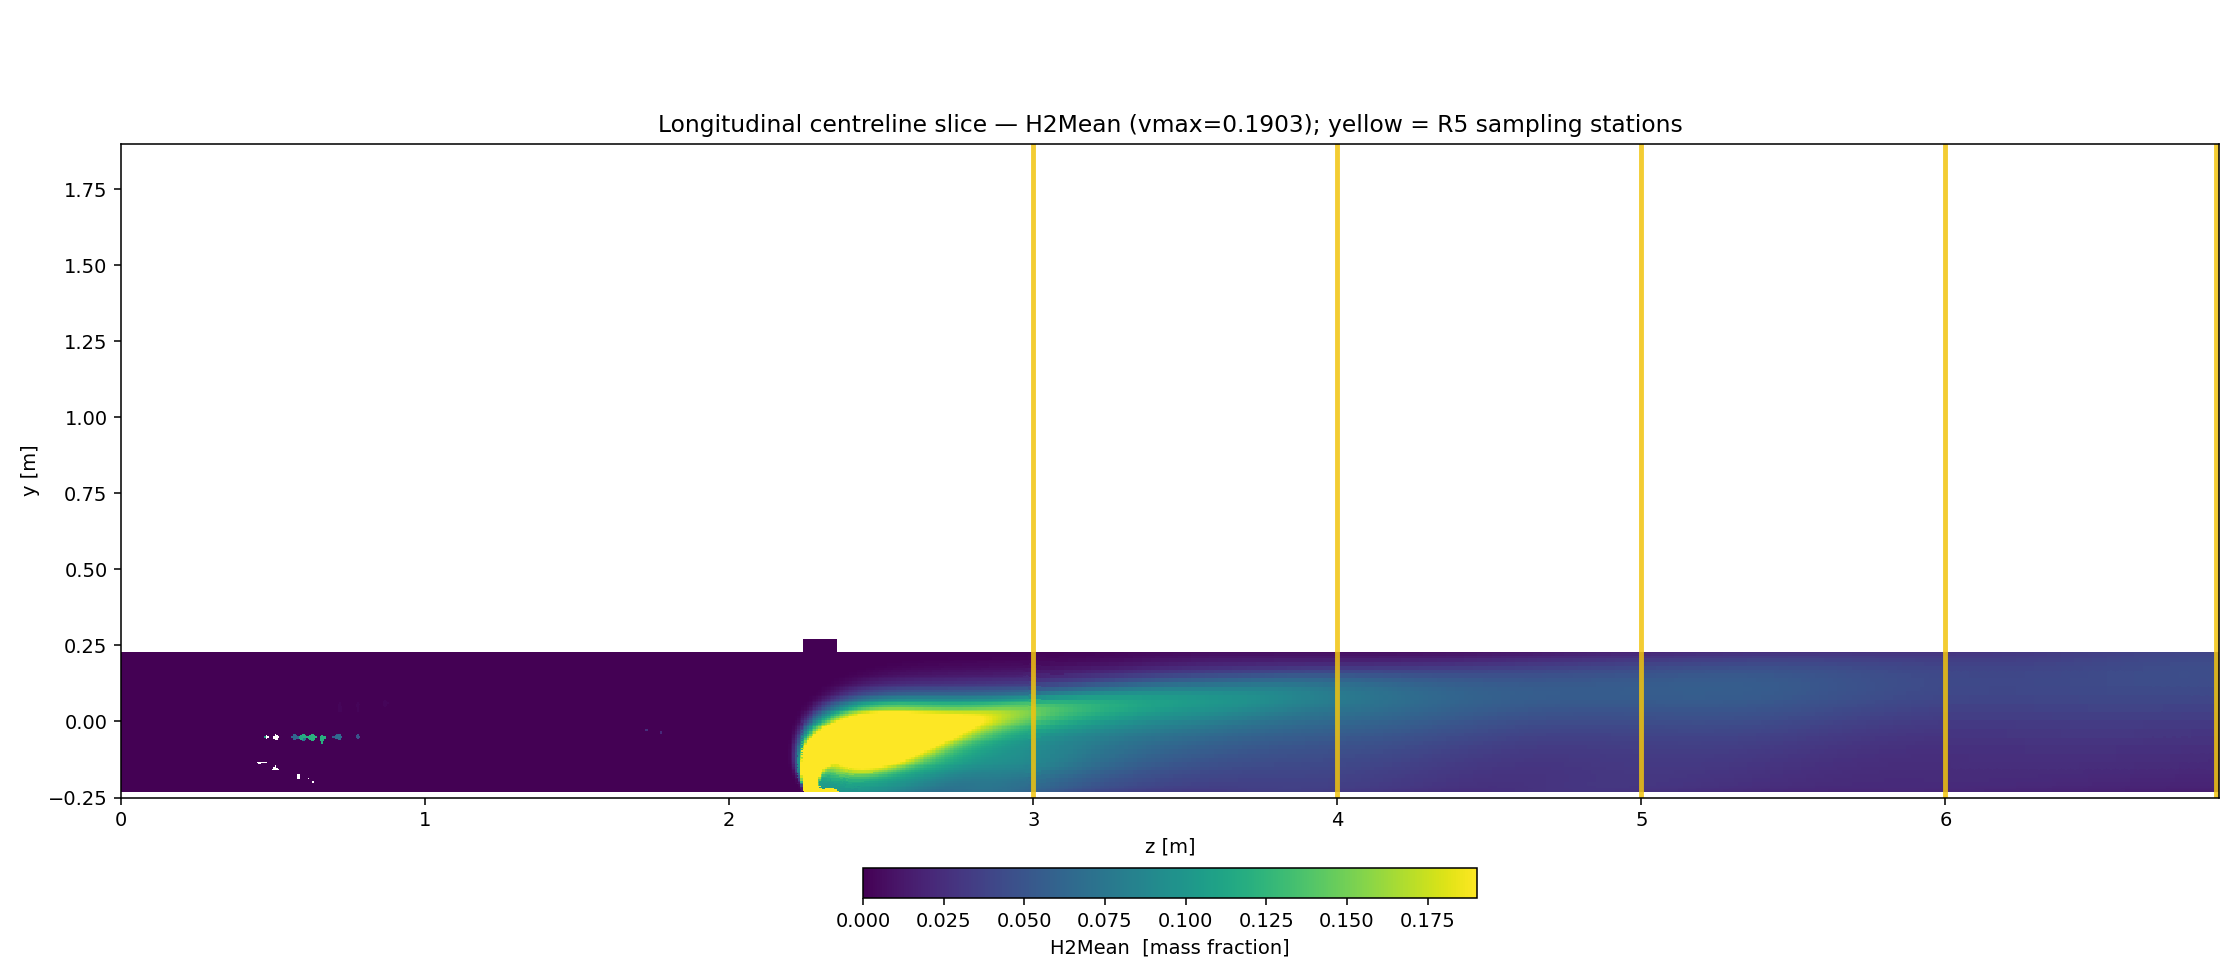
\includegraphics[width=0.85\textwidth]{../doe/results_full_90deg_bottom/case_04/figures/fig_H2_long.png}
        \caption{Bottom injection --- plume hugs the bottom wall and
        rises as a narrow column.}
    \end{subfigure}
    \caption{Longitudinal centreline \(Y_{\Hi}\) for case~04
    at \(90^\circ\).}
    \label{fig:bot_long_04}
\end{figure}

% =====================================================================
%  9. FOUR-CAMPAIGN SYNTHESIS  (condensed)
% =====================================================================
\section{Cross-campaign synthesis: injection side}
\label{sec:cross_side}

All 40 valid cases are now compared.

\subsection{CoV vs VR: four-campaign power-law}
\label{sec:cross4_vr}
The fits (Fig.~\ref{fig:cross4_cov_vr}) are:
\(90^\circ\) top: \(\CoV\approx 0.47\,\VR^{-1.16}\) (\(R^2=0.80\));
\(30^\circ\) top: \(0.33\,\VR^{-1.88}\) (\(0.80\));
\(90^\circ\) bot: \(0.89\,\VR^{-0.91}\) (\(0.90\));
\(30^\circ\) bot: \(1.13\,\VR^{-0.72}\) (\(0.72\)).
Top-injection exponents are steeper; intercepts are lower.

\begin{figure}[H]
    \centering
    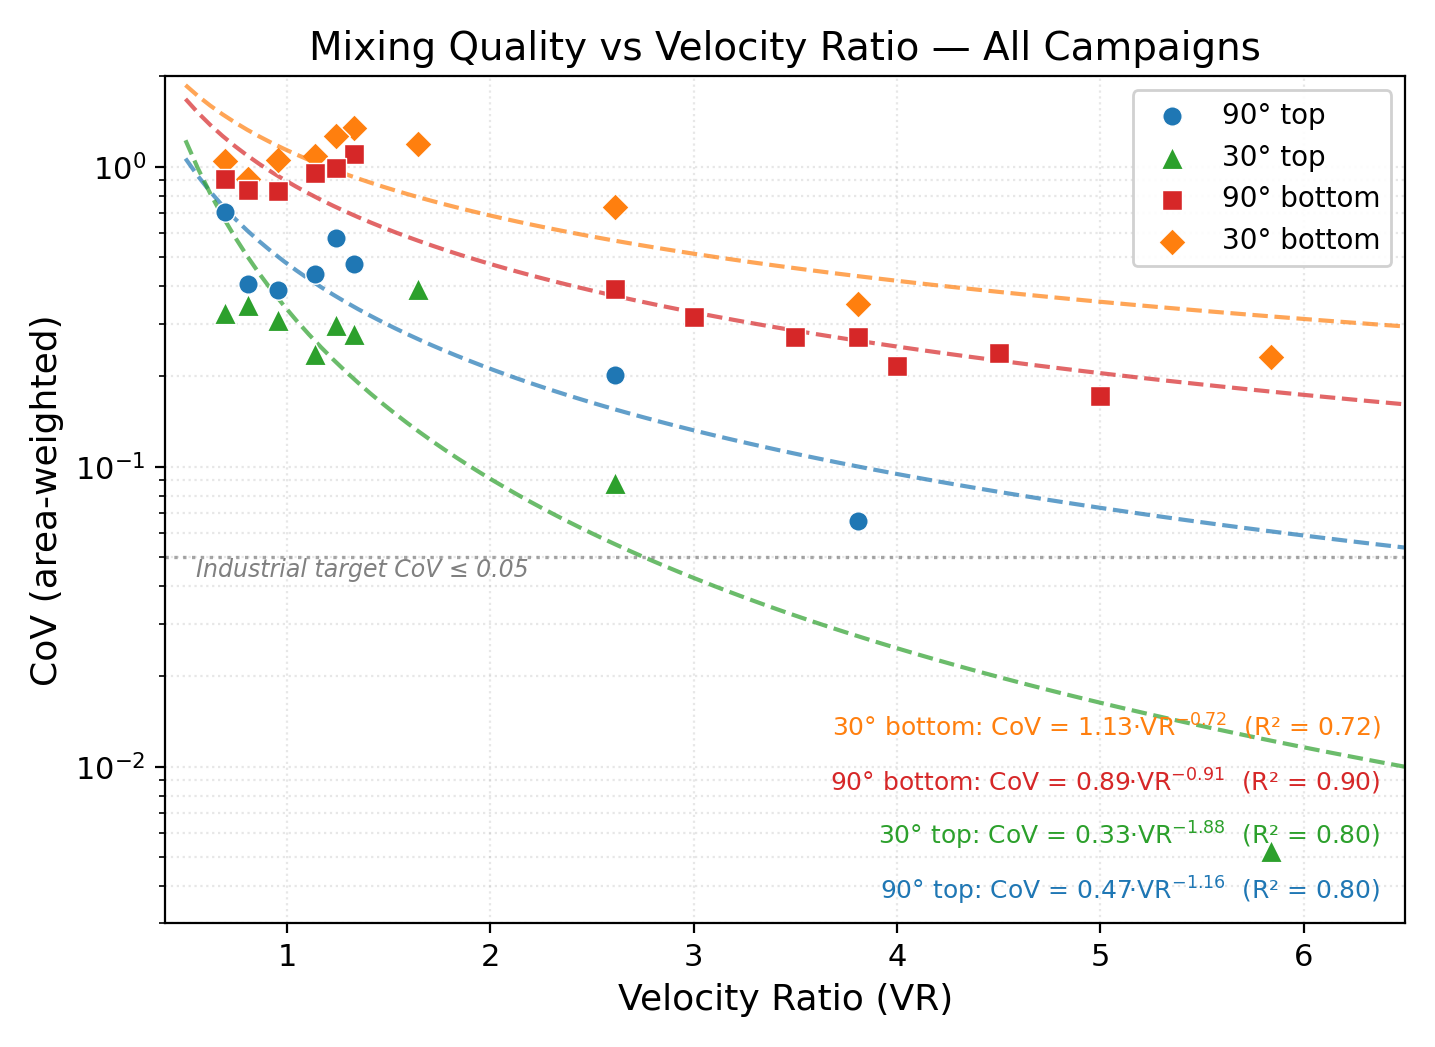
\includegraphics[width=0.78\textwidth]{../doe/cross_campaign/figures/fig1_CoV_vs_VR.png}
    \caption{Power-law \CoV{} vs.\ \VR{} for all four campaigns.}
    \label{fig:cross4_cov_vr}
\end{figure}

\subsection{Matched-pair: top vs bottom}
\label{sec:cross4_pairs}
In \textbf{all 17} matched pairs (8 at \(90^\circ\), 9 at
\(30^\circ\)), top injection achieves lower \CoV{}
(Fig.~\ref{fig:cross4_matched}).
Median degradation top\(\to\)bottom: \(+109\,\%\) at \(90^\circ\),
\(+324\,\%\) at \(30^\circ\).
Probability under null: \(2^{-17}=1.5\times 10^{-5}\).

\begin{figure}[H]
    \centering
    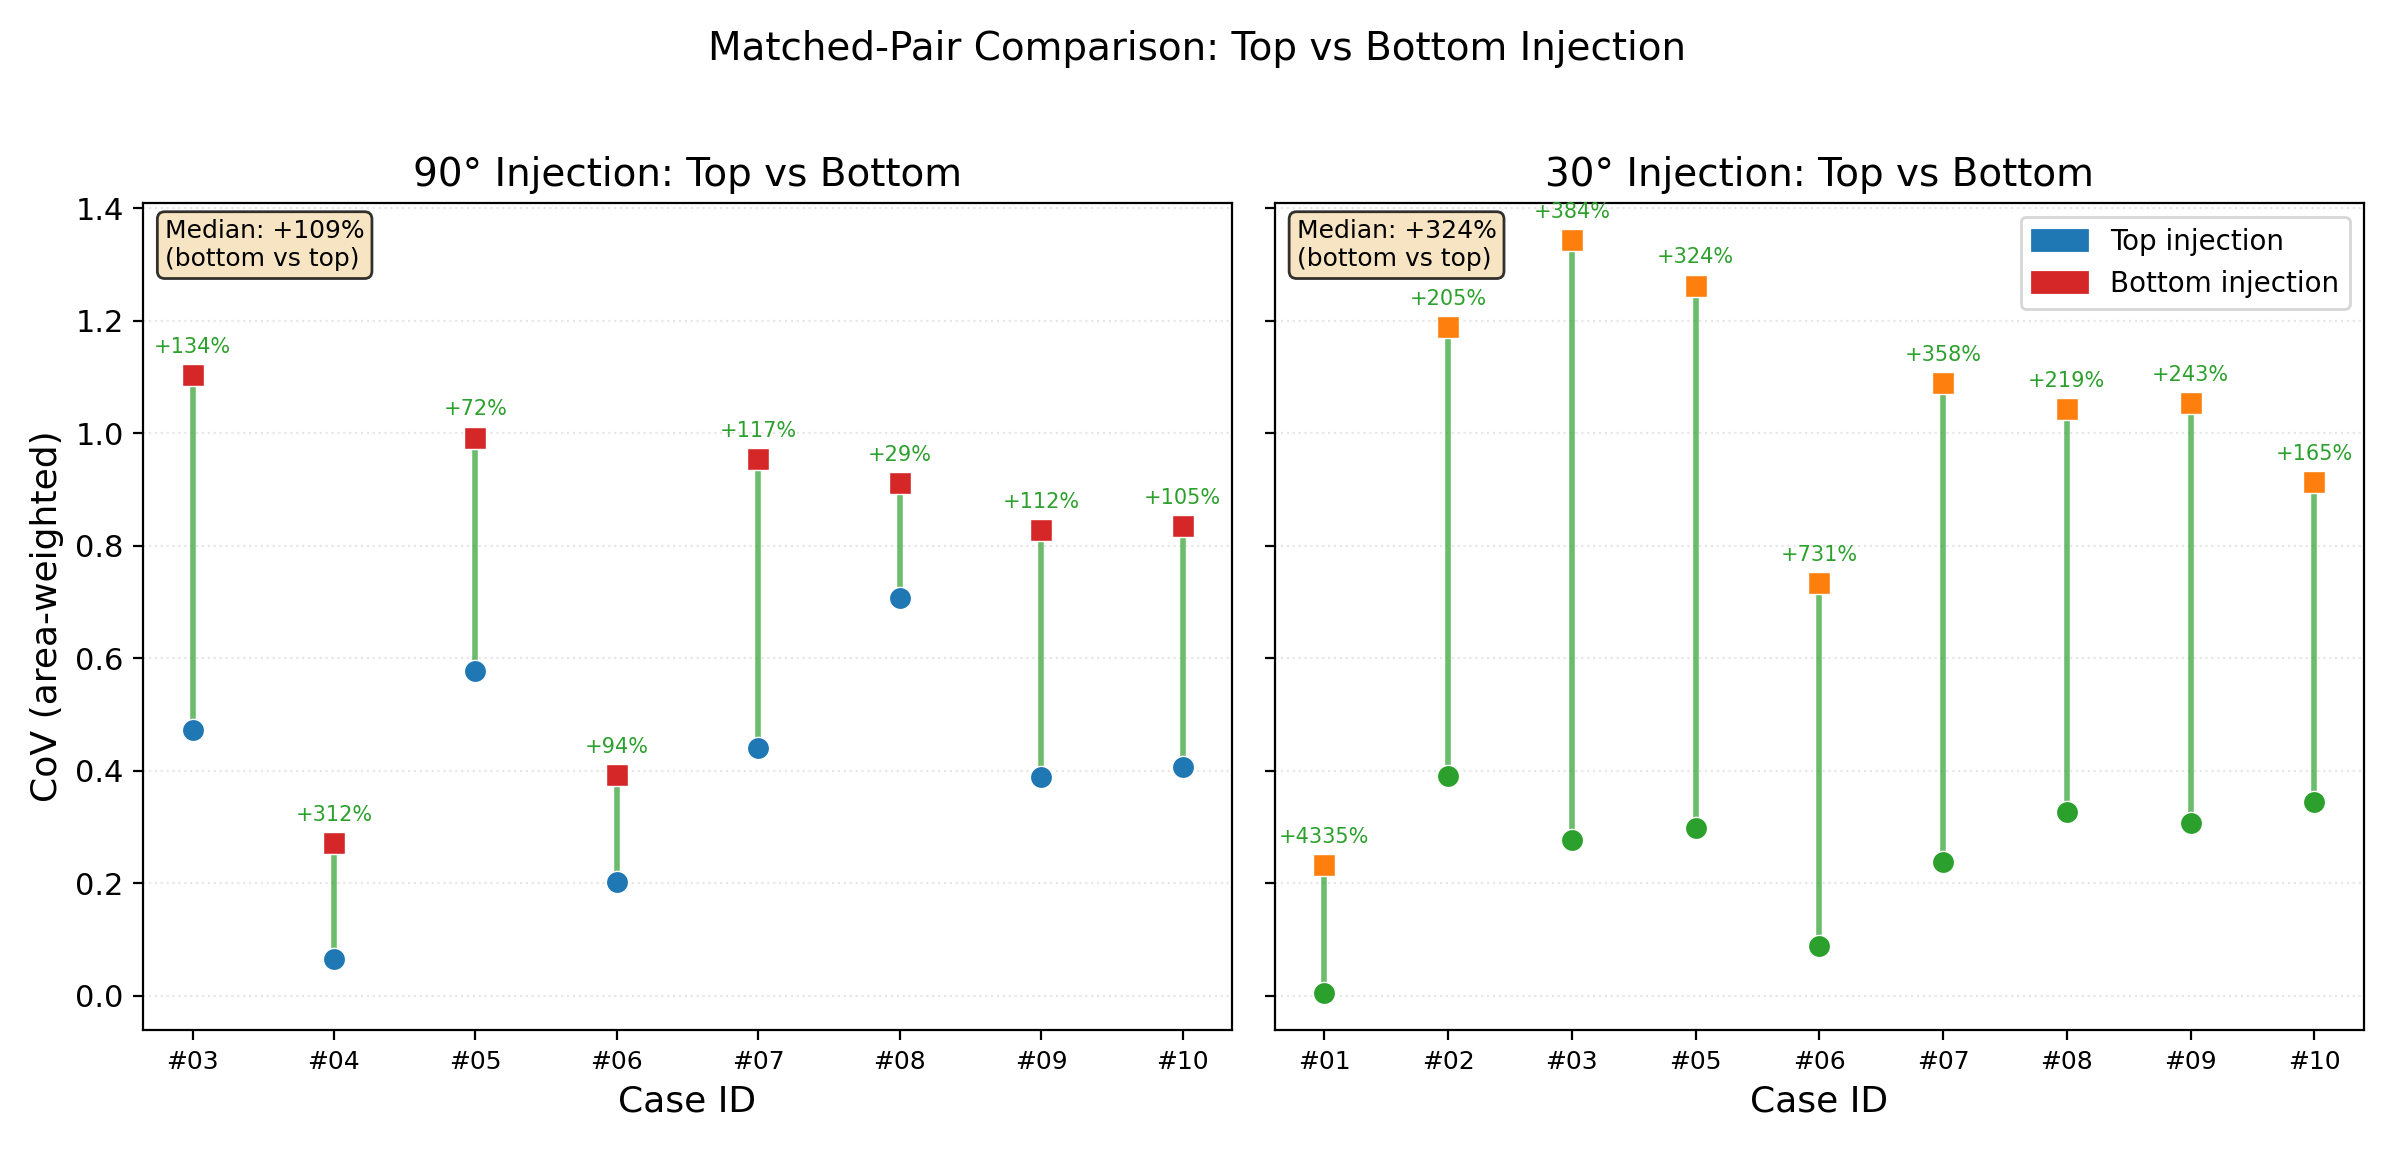
\includegraphics[width=0.85\textwidth]{../doe/cross_campaign/figures/fig2_matched_pairs_top_vs_bottom.png}
    \caption{Top vs.\ bottom matched-pair arrows. Every arrow shows
    bottom injection is worse.}
    \label{fig:cross4_matched}
\end{figure}

\subsection{Pressure-drop trends}
\label{sec:cross4_dp}
LP-filtered \(|\Delta p|\) medians are
\SI{1.05}{\kilo\pascal} (\(90^\circ\)~top),
\SI{0.53}{\kilo\pascal} (\(30^\circ\)~top),
\SI{1.58}{\kilo\pascal} (\(90^\circ\)~bot),
\SI{1.02}{\kilo\pascal} (\(30^\circ\)~bot) ---
all within a \(\sim\SI{1}{\kilo\pascal}\) band.

\textbf{Injection side does not affect \(|\Delta p|\).}
The junction pressure loss is set by the local momentum budget
(area expansion and turning) at the T-junction, which depends on
\((\dD)^2\) and the geometric angle \(\alpha\); flipping the
branch from top to bottom changes the buoyancy force on the
\emph{downstream} plume but not the junction geometry, so
\(K=|\Delta p|/q_{\mathrm{dyn,main}}\) is unchanged.

\textbf{The \(30^\circ\) tilt reduces \(|\Delta p|\).}
Comparing at the same injection side:
\(30^\circ\)~top (\SI{0.53}{\kilo\pascal}) is roughly half of
\(90^\circ\)~top (\SI{1.05}{\kilo\pascal}).
The branch jet at \(30^\circ\) enters with a large streamwise
momentum component and only turns through \(30^\circ\) instead
of \(90^\circ\); the \(60^\circ\) of saved turning loss is
never generated, consistent with \citet{idelchik1986handbook}.

\textbf{\(|\Delta p|\) vs \VR.}
For top injection, \(|\Delta p|\) increases with \VR{} (higher
branch dynamic pressure); for bottom injection the correlation
breaks down because the coherent buoyant plume redistributes
pressure in ways that do not scale simply with \VR.

\begin{figure}[H]
    \centering
    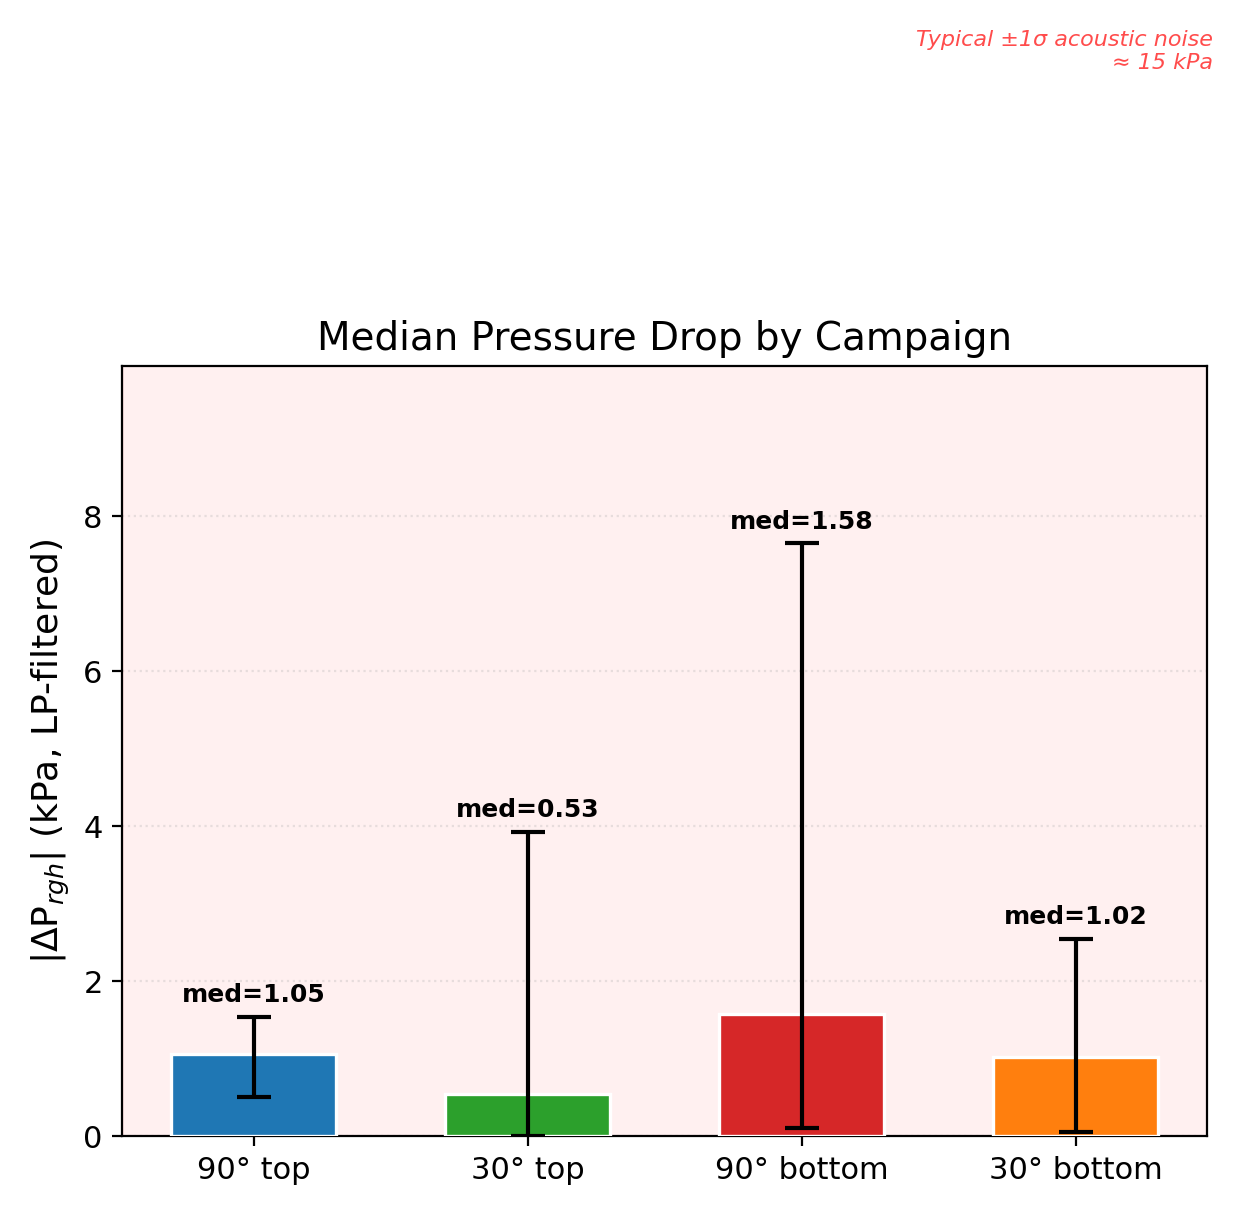
\includegraphics[width=0.65\textwidth]{../doe/cross_campaign/figures/fig11_bar_median_dP.png}
    \caption{Median LP-filtered \(|\Delta p|\) by campaign.
    The \(30^\circ\) tilt halves the pressure drop relative to
    \(90^\circ\).}
    \label{fig:cross4_bar_dP}
\end{figure}

\begin{figure}[H]
    \centering
    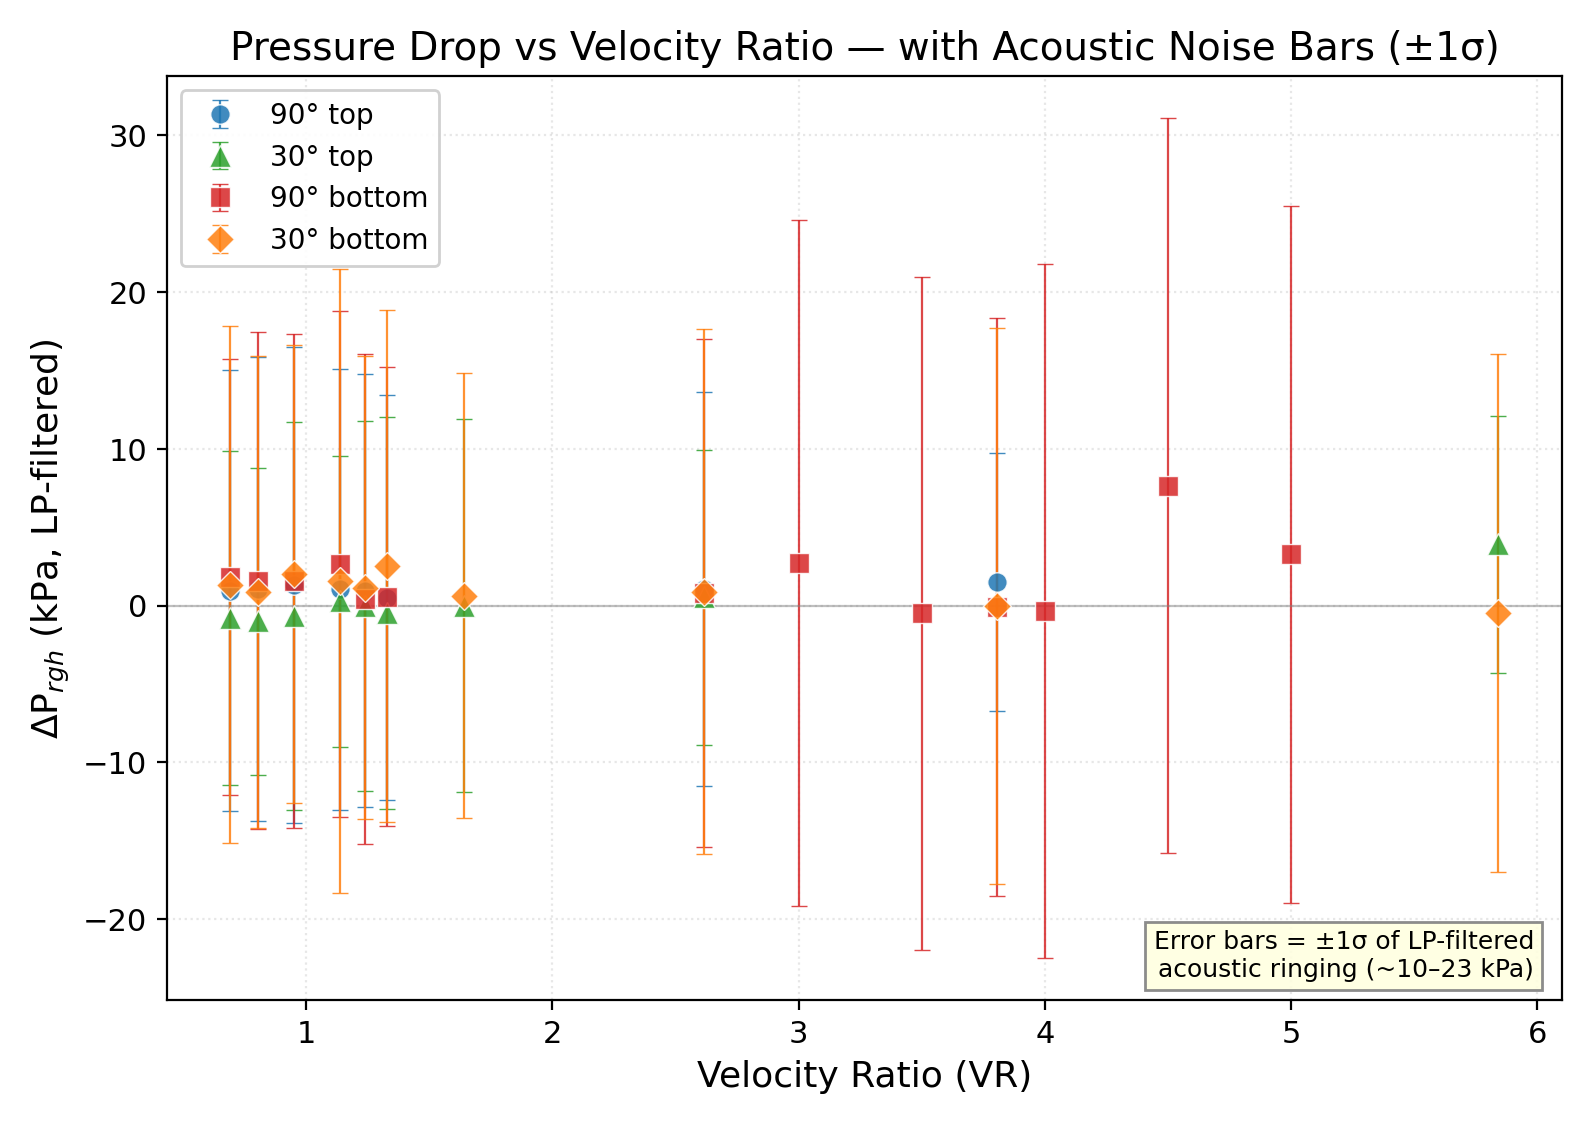
\includegraphics[width=0.78\textwidth]{../doe/cross_campaign/figures/fig8_dP_vs_VR_errorbars.png}
    \caption{\(|\Delta p|\) vs.\ \VR{} with per-case LP-filter
    uncertainty bars.  Top-injection campaigns show a clear
    positive trend; bottom campaigns are scattered.}
    \label{fig:cross4_dP_VR}
\end{figure}

\subsection{Acoustic noise in the pressure signal}
\label{sec:cross4_noise}
The compressible solver generates standing acoustic waves between
the reflecting inlet and outlet patches.  The peak-to-trough
amplitude reaches \(\sim\SI{25}{\kilo\pascal}\), dwarfing the
between-case \(|\Delta p|\) signal (\(\sim\SI{1}{\kilo\pascal}\)).
Figure~\ref{fig:cross4_acoustic} shows the ratio of acoustic
amplitude to the LP-filtered \(|\Delta p|\) as a function of
\VR{}, underscoring why the \(\Delta p\) surrogate fails.

\begin{figure}[H]
    \centering
    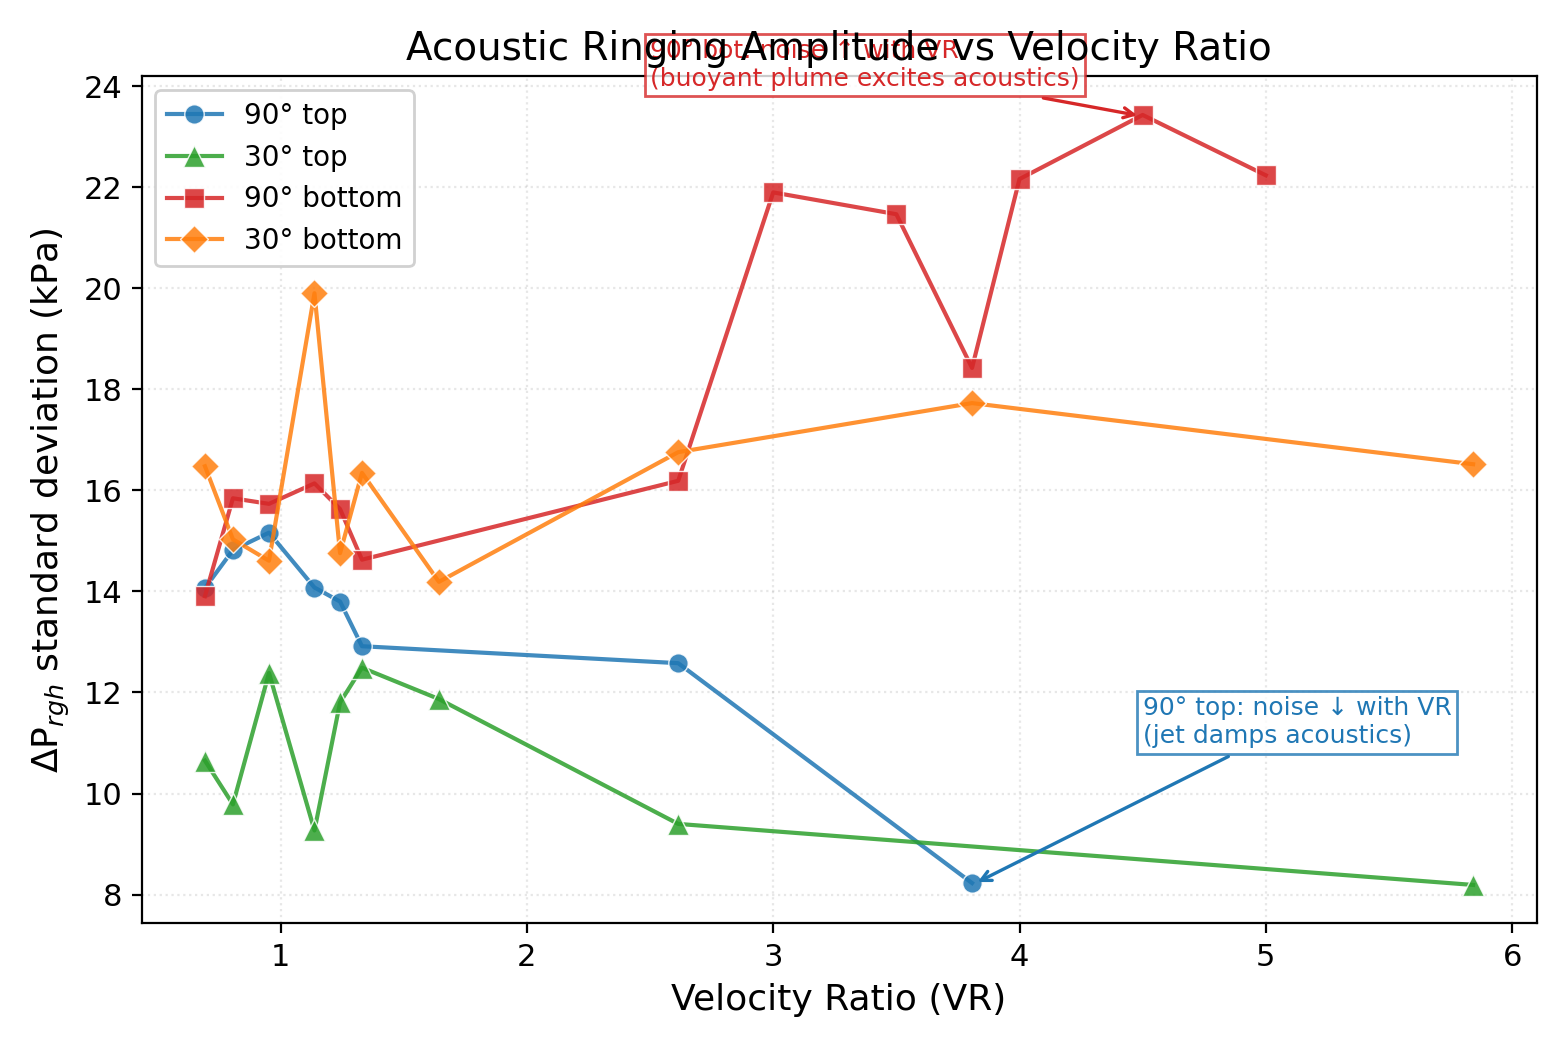
\includegraphics[width=0.75\textwidth]{../doe/cross_campaign/figures/fig9_acoustic_noise_vs_VR.png}
    \caption{Acoustic-to-signal ratio for \(|\Delta p|\).
    Values above 1 (red dashed line) indicate that the noise
    exceeds the true pressure drop.}
    \label{fig:cross4_acoustic}
\end{figure}

\subsection{Pareto front: four campaigns}
\label{sec:cross4_pareto}
The four-campaign Pareto (Fig.~\ref{fig:cross4_pareto}) confirms
that top-injection points dominate the lower-left corner; no
bottom-injection point reaches \(\CoV\le 0.05\).

\begin{figure}[H]
    \centering
    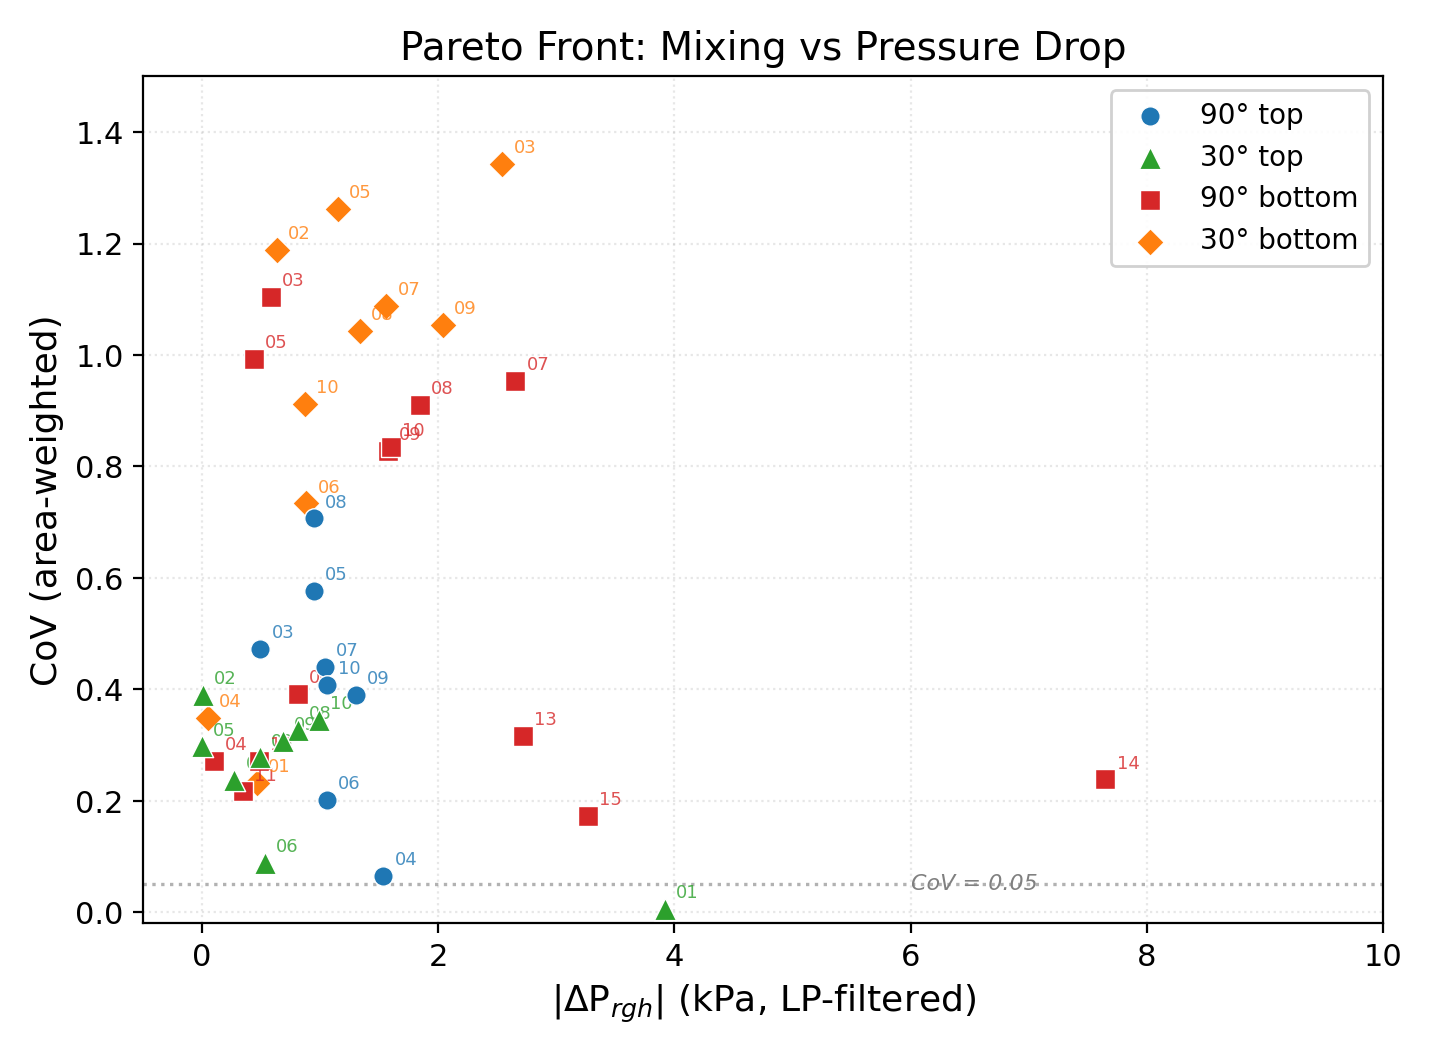
\includegraphics[width=0.78\textwidth]{../doe/cross_campaign/figures/fig3_pareto.png}
    \caption{Four-campaign Pareto front.  Top-injection points
    cluster in the desirable lower-left region.}
    \label{fig:cross4_pareto}
\end{figure}

\subsection{Design-space heatmap}
Figure~\ref{fig:cross4_heatmap} shows a \(2\times 2\) grid of
\CoV{} heatmaps in \((\dD,\VR)\) space.
The bottom row is uniformly darker (higher \CoV) than the top row,
making the injection-side effect visually immediate.

\begin{figure}[H]
    \centering
    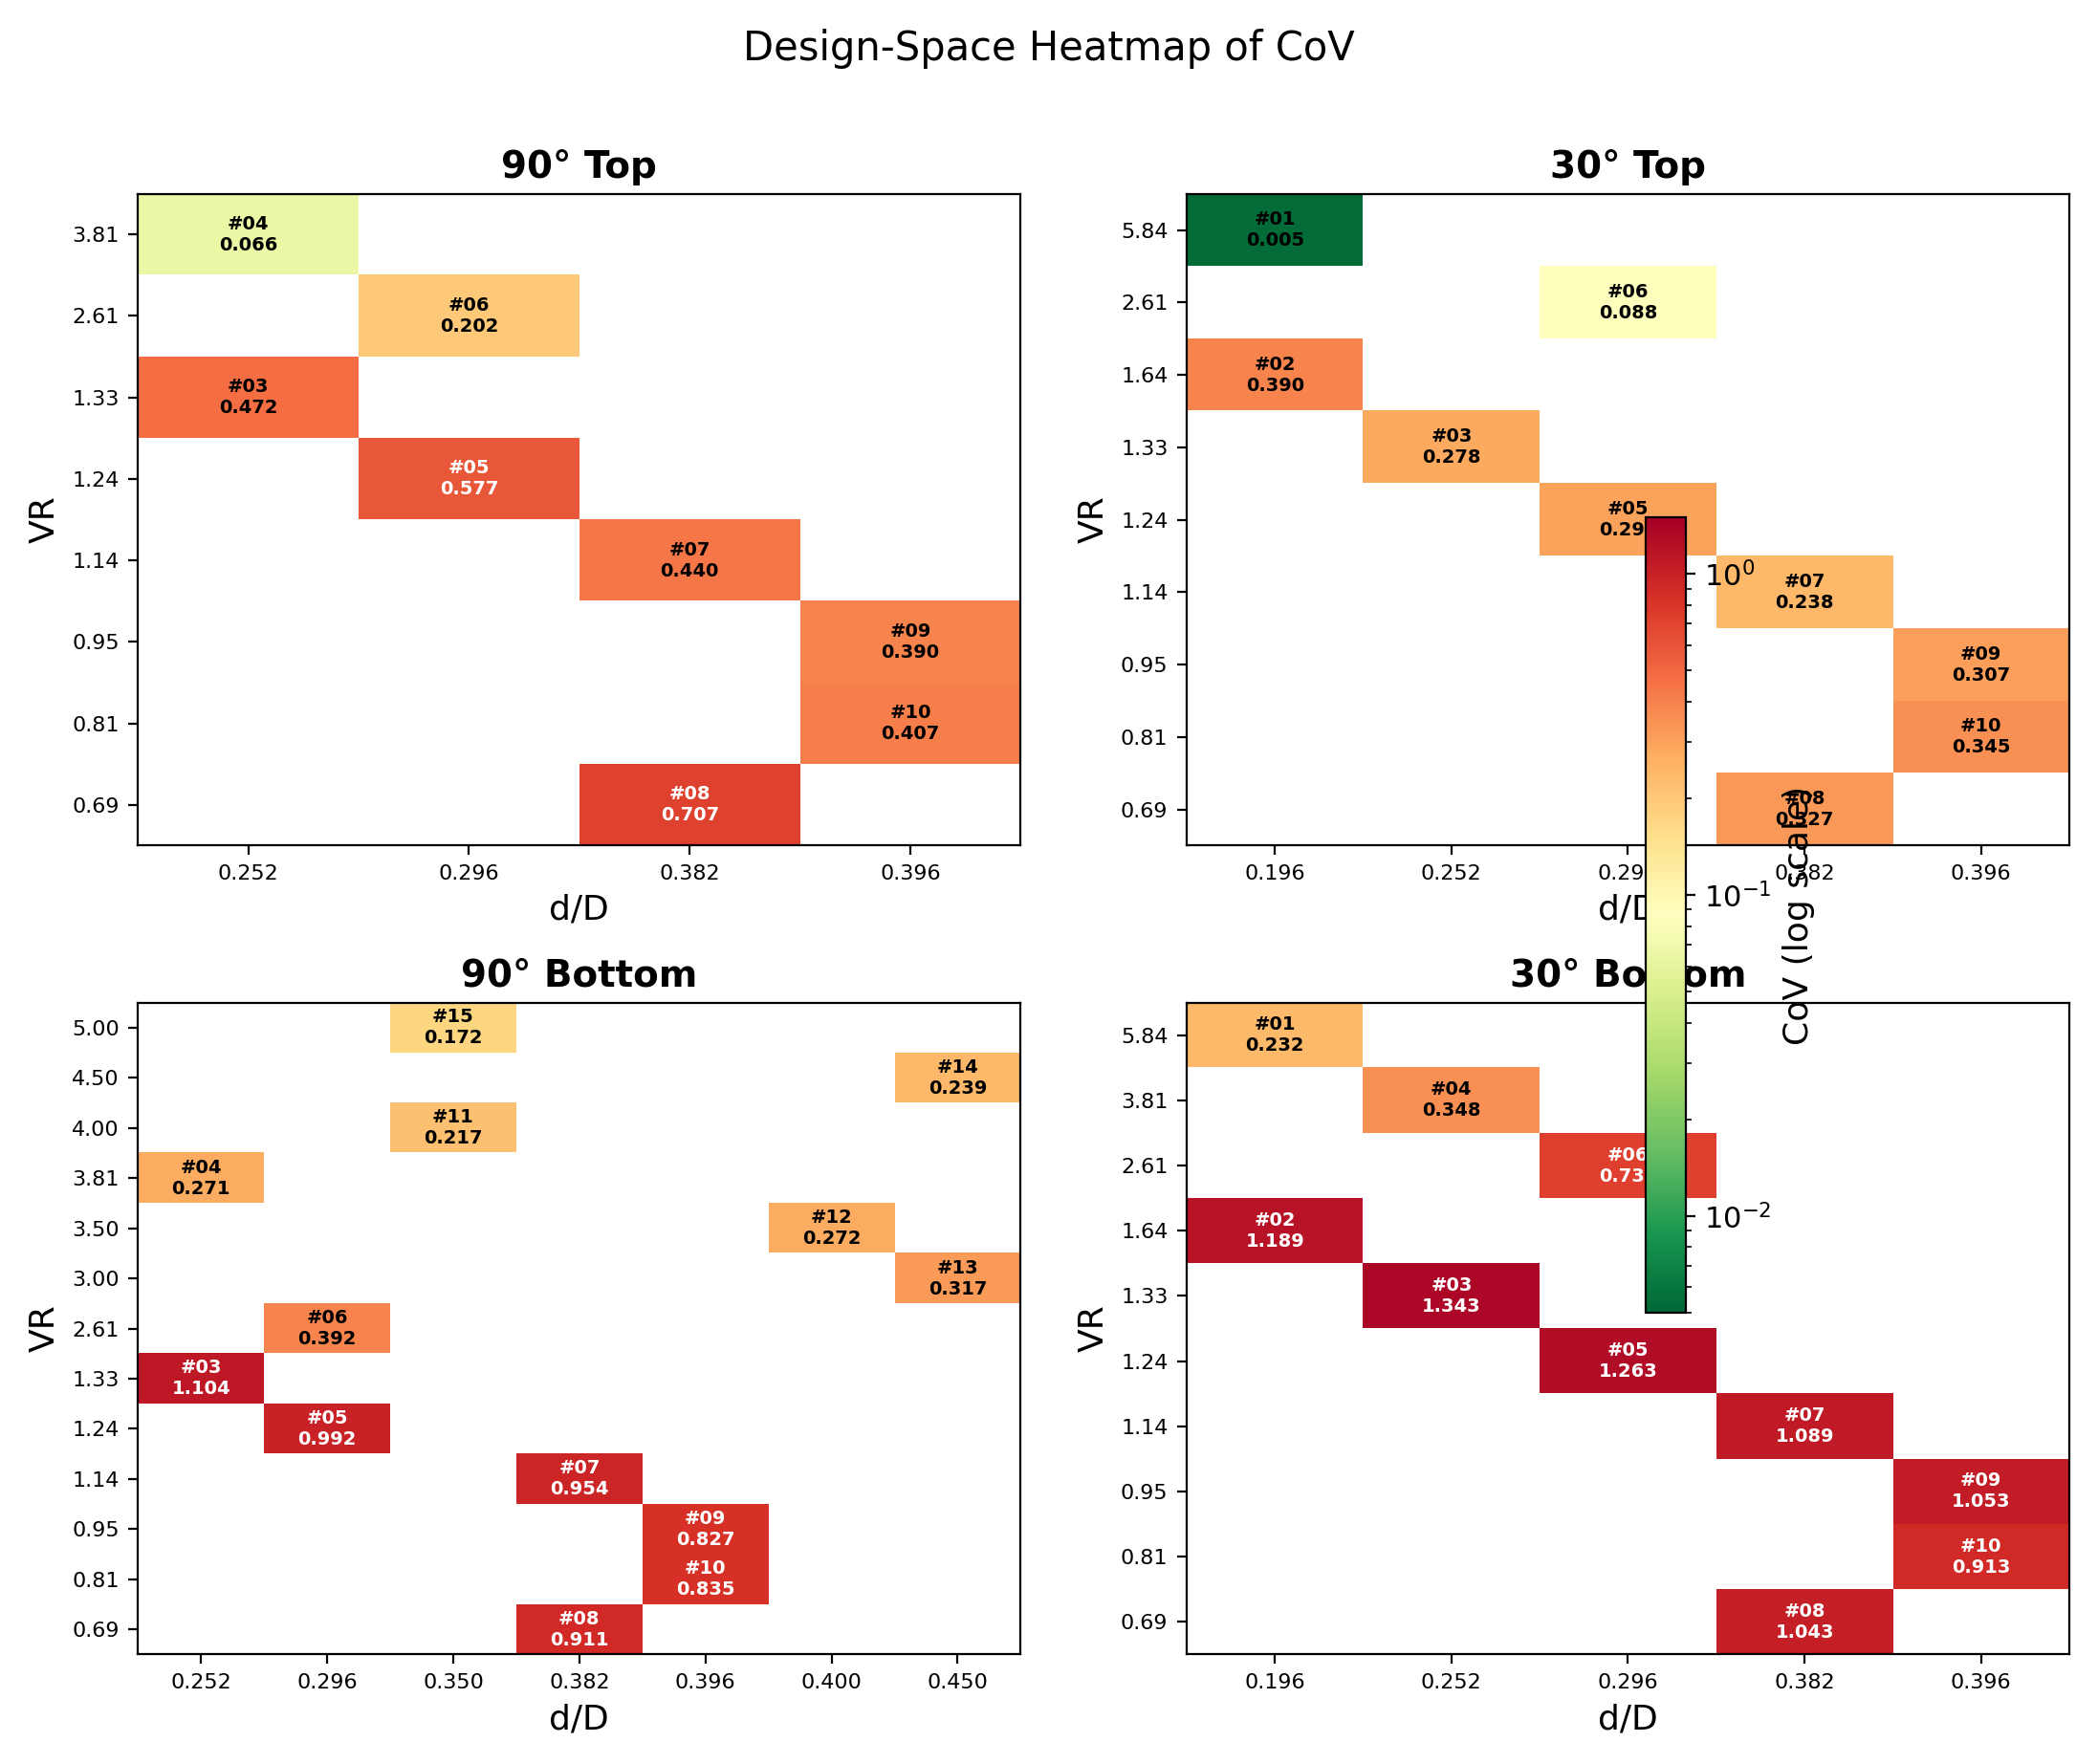
\includegraphics[width=0.85\textwidth]{../doe/cross_campaign/figures/fig4_heatmap_CoV.png}
    \caption{Design-space heatmap of \CoV{}.  Columns:
    \(90^\circ\)/\(30^\circ\).  Rows: top/bottom.  Log colour
    scale, shared.}
    \label{fig:cross4_heatmap}
\end{figure}

\subsection{Executive summary}
The median \CoV{} bar chart (Fig.~\ref{fig:cross4_bar}) distils
the dataset: \(30^\circ\) top is best (median \(\CoV=0.298\));
\(30^\circ\) bottom is worst (\(1.048\)).  Even the best
bottom-injection case barely approaches the worst top-injection
case.

\begin{figure}[H]
    \centering
    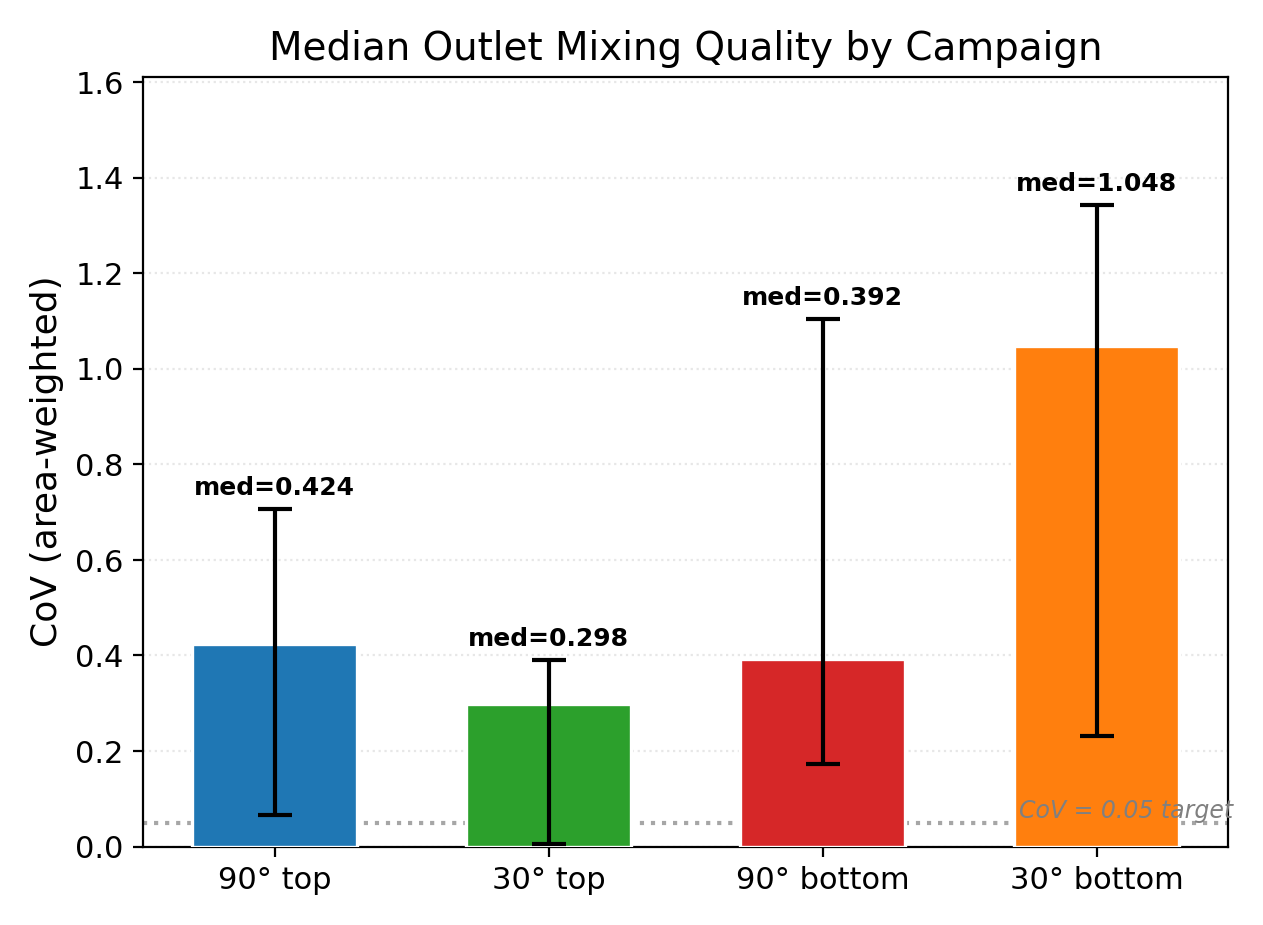
\includegraphics[width=0.65\textwidth]{../doe/cross_campaign/figures/fig5_bar_median_CoV.png}
    \caption{Median \CoV{} by campaign with min--max bars.
    Dashed line: \(\CoV=0.05\) target.}
    \label{fig:cross4_bar}
\end{figure}

\subsection{Physical mechanism: buoyancy effect on plume structure}
\label{sec:cross4_mech}

The quantitative superiority of top injection has a clear physical
explanation, illustrated in Fig.~\ref{fig:cross4_mechanism}.

\begin{figure}[H]
    \centering
    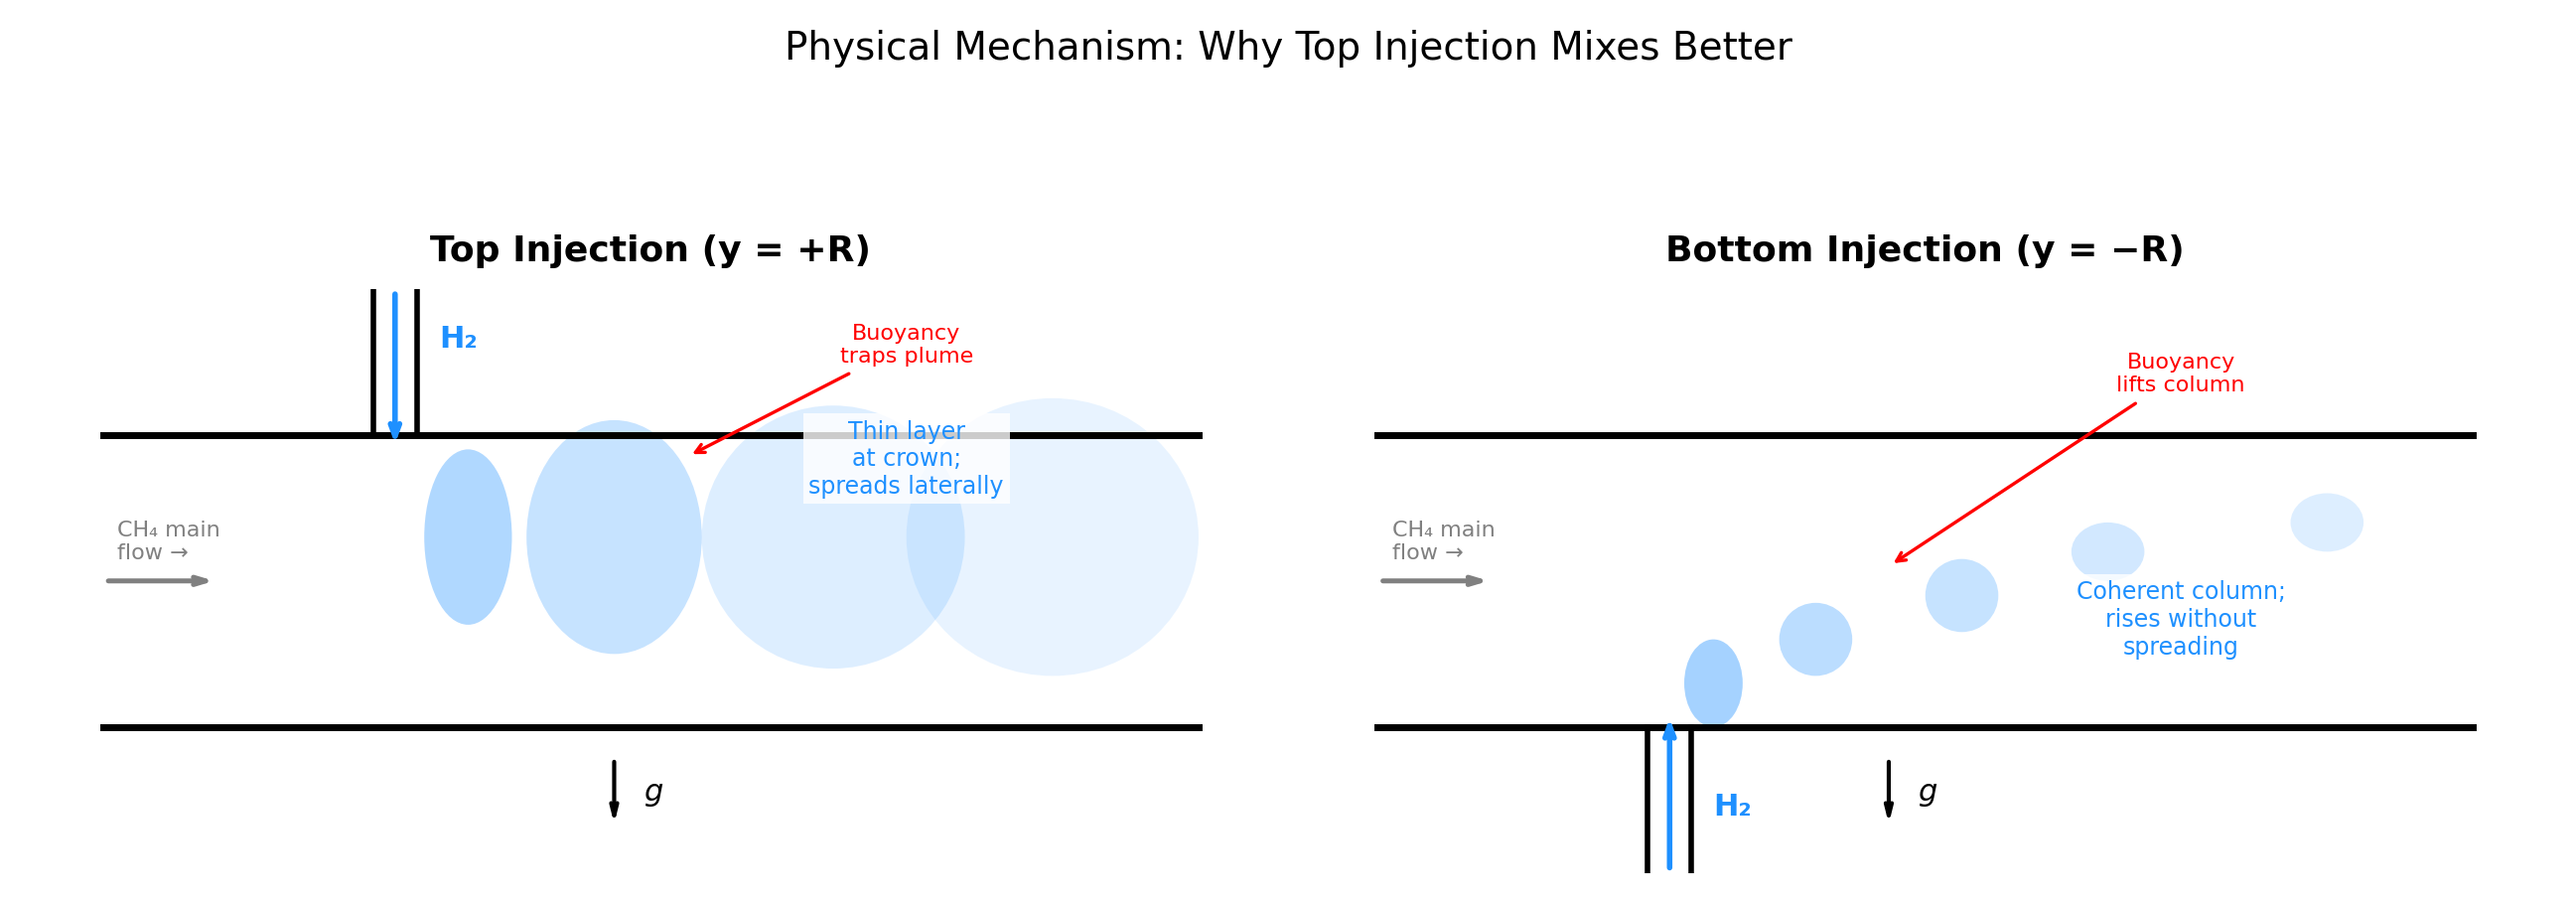
\includegraphics[width=0.85\textwidth]{../doe/cross_campaign/figures/fig6_mechanism_schematic.png}
    \caption{Schematic of the buoyancy mechanism.  Left: top
    injection spreads \Hi{} laterally along the crown.
    Right: bottom injection lifts the plume as a coherent column.}
    \label{fig:cross4_mechanism}
\end{figure}

When \Hi{} is injected from the top, the jet penetrates downward;
buoyancy prevents the lighter gas from sinking further and spreads
it laterally along the pipe crown, creating a thin layer with
large interfacial area for turbulent diffusion.
When injected from the bottom, buoyancy \emph{assists} the jet:
the light gas rises as a coherent column without fanning out.
By the outlet, the \Hi{} occupies a concentrated streak rather
than being distributed across the full cross-section.

The \(30^\circ\) bottom campaign is worst of all four because
the co-flow angle reduces jet penetration \emph{and} enters
the pipe nearly tangentially from below, giving buoyancy maximum
leverage to lift the coherent plume before spreading.

Figure~\ref{fig:cov_zD_topbot} compares the \CoV{} decay for
case~04 top vs.\ bottom: top injection decays steeply to
\(\sim\!0.07\); bottom plateaus at \(\sim\!0.28\).

\begin{figure}[H]
    \centering
    \begin{minipage}[t]{0.48\textwidth}
       \centering
       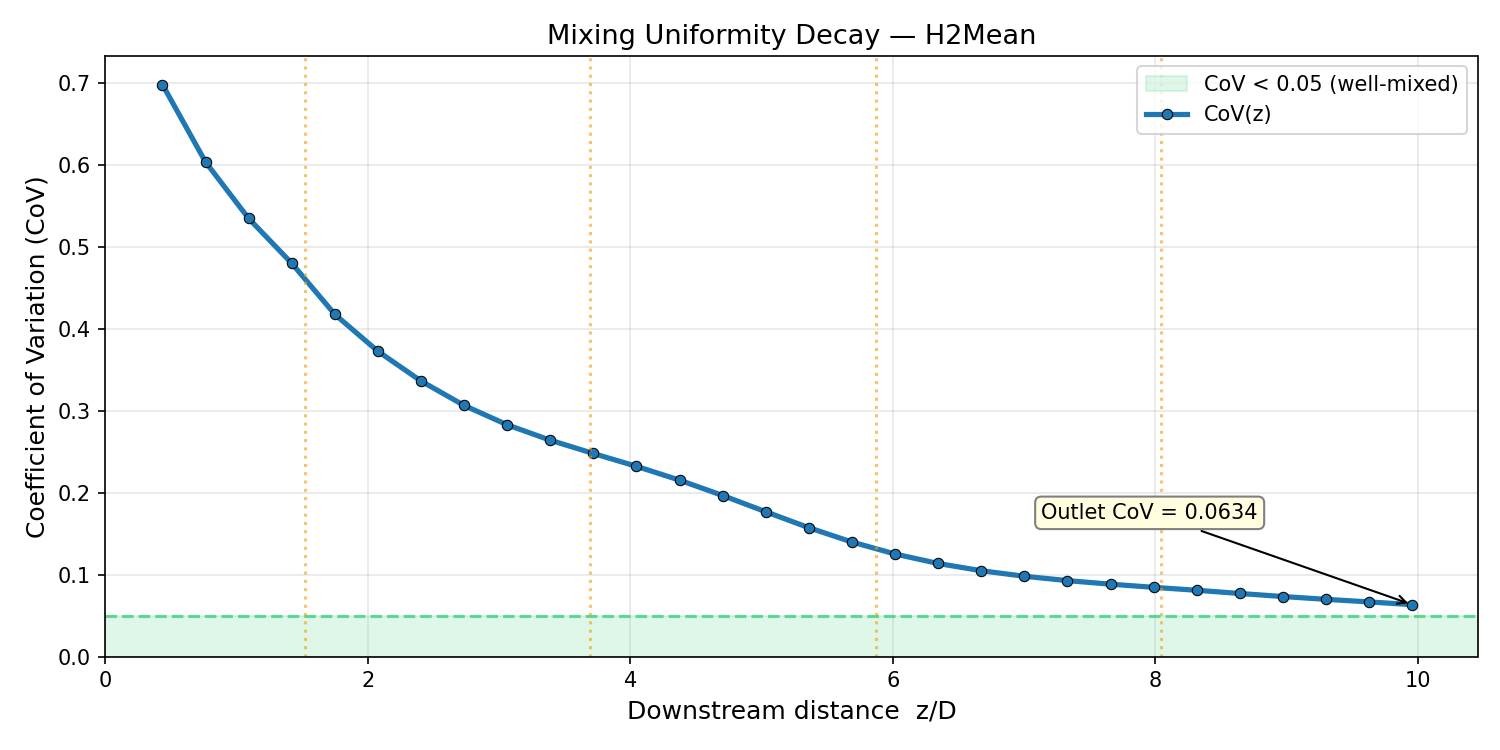
\includegraphics[width=\textwidth]{../doe/results_full/cases/case_04/figures/fig_CoV_vs_zD.png}
    \end{minipage}\hfill
    \begin{minipage}[t]{0.48\textwidth}
       \centering
       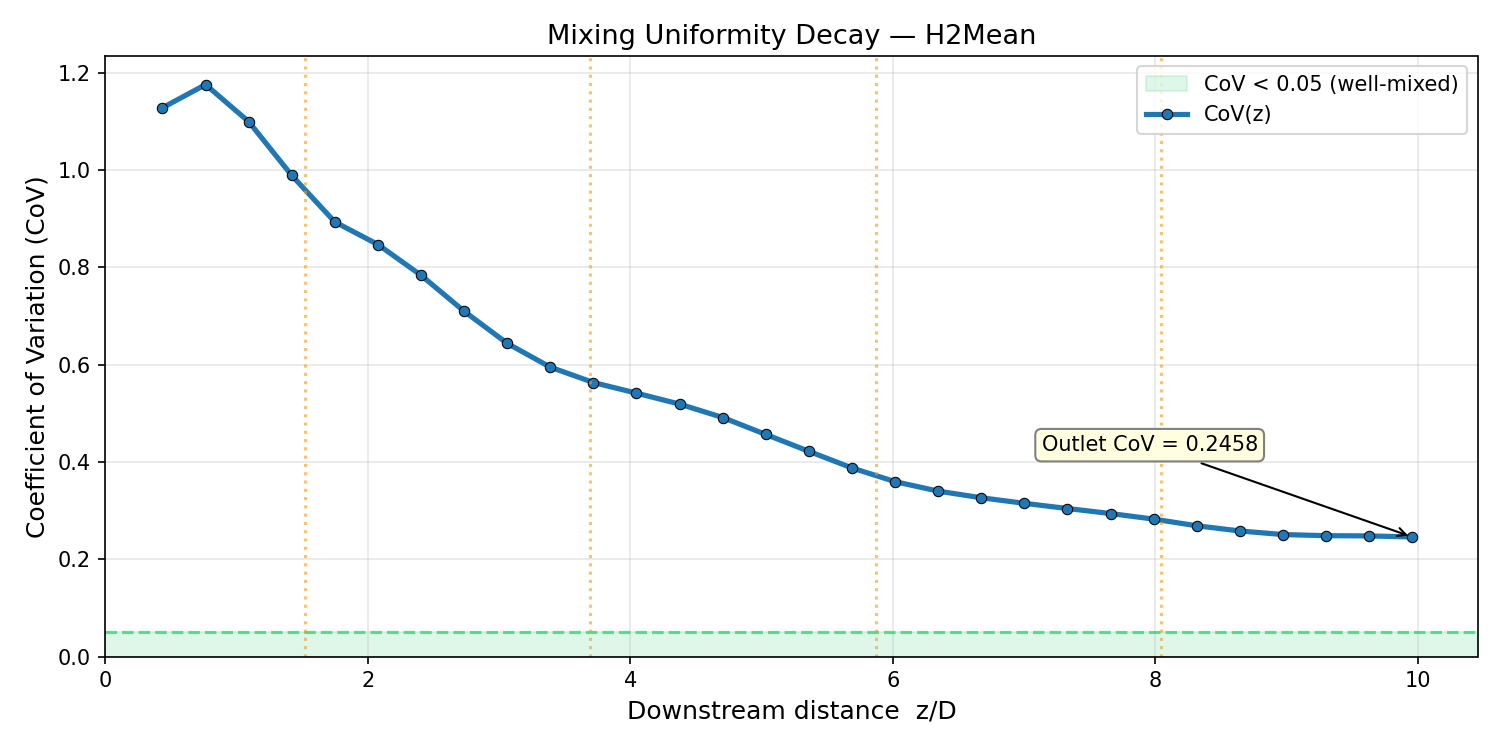
\includegraphics[width=\textwidth]{../doe/results_full_90deg_bottom/case_04/figures/fig_CoV_vs_zD.png}
    \end{minipage}
    \caption{\CoV{} vs.\ \(z/D\) for case~04 (\(\VR=3.81\))
    at \(90^\circ\): top (left) vs.\ bottom (right).
    Green band = \(\CoV<0.05\).}
    \label{fig:cov_zD_topbot}
\end{figure}

\subsection{Effect of \texorpdfstring{$d/D$}{d/D} at fixed VR}
\label{sec:cross4_dD}
Across all four campaigns at low \VR{} (0.6--1.5), larger
\(\dD\) tends to produce marginally lower \CoV{}
(Fig.~\ref{fig:cross4_dD}), consistent with
\citet{su2022prediction}.  The effect is secondary to both
\VR{} and injection side.

\begin{figure}[H]
    \centering
    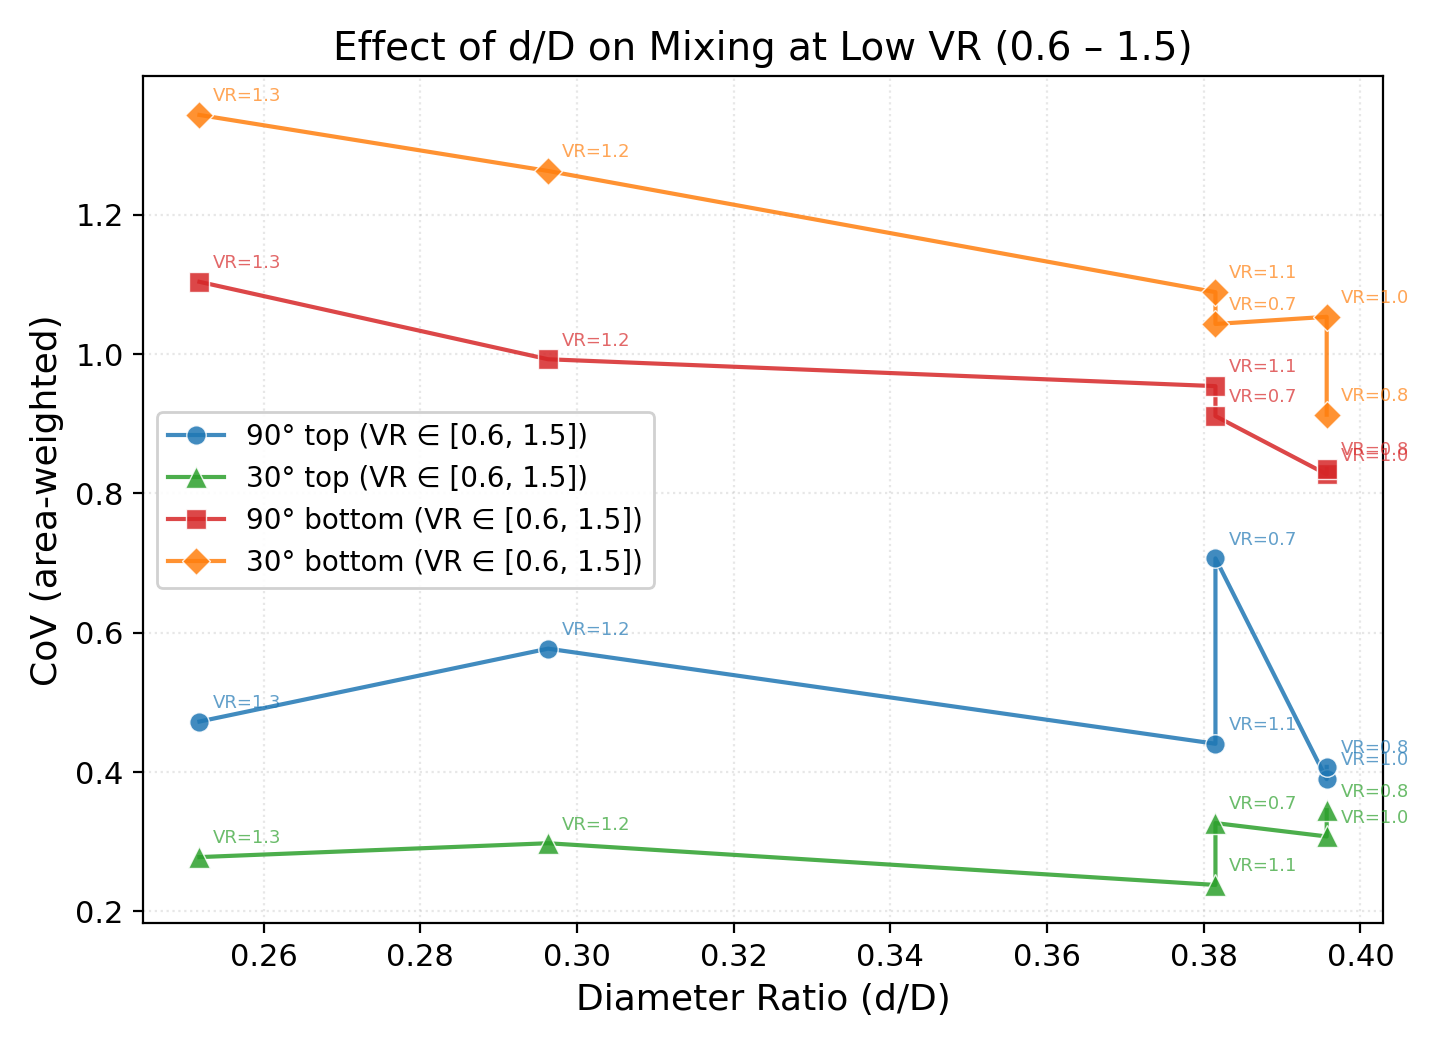
\includegraphics[width=0.75\textwidth]{../doe/cross_campaign/figures/fig7_CoV_vs_dD.png}
    \caption{\CoV{} vs.\ \(\dD\) at low \VR.  Downward trend
    is weak but consistent.}
    \label{fig:cross4_dD}
\end{figure}

% =====================================================================
%  10. SURROGATE MODELLING  (condensed)
% =====================================================================
\section{Surrogate modelling and optimisation}
\label{sec:surrogate}

The 40-case dataset is used to train surrogates that approximate
\((\alpha,\dD,\VR,\HBR,\text{side})\to(\CoV,|\Delta p|)\).
Features are encoded as a 6-D vector (one-hot injection side,
MinMax-scaled continuous variables).

\subsection{Models compared}
Four architectures were benchmarked
(Table~\ref{tab:surrogate_error}):
\begin{enumerate}
   \item \textbf{DNN}:
         \(6\!\to\!64\!\to\!128\!\to\!64\!\to\!32\!\to\!2\),
         ReLU, Adam (\(\eta=10^{-3}\), L\(_2\) reg.),
         early stopping; 5-fold CV.
   \item \textbf{GPR}: Mat\'ern-5/2 kernel with ARD, 10 restarts;
         LOO-CV.
   \item \textbf{Random Forest}: 200 trees,
         \(\texttt{min\_samples\_leaf}=2\); LOO-CV.
   \item \textbf{Gradient Boosting}: 200 estimators,
         depth~3, \(\eta=0.05\); LOO-CV.
\end{enumerate}

\noindent\textbf{Key findings:}
(i)~GPR achieves \(R^{2}=0.93\) for \CoV{} (MAE~0.083 on a
\([0.005,\,1.34]\) range), confirming that the design variables
encode the dominant mixing physics.
(ii)~The DNN overfits at \(N\!=\!40\)
(\(\sim\!17\,400\) parameters vs.\ 40 samples; \(R^{2}=0.74\));
the architecture was designed for the planned 420-case DoE.
(iii)~No model predicts \(\Delta p\)
(\(R^{2}\!\approx\!0\)) because the per-case acoustic noise
(\(\pm\SI{10}{\kilo\pascal}\)) dwarfs the
\(\lesssim\SI{2}{\kilo\pascal}\) between-case signal.

\begin{table}[H]
\centering\scriptsize
\caption{Cross-validated surrogate accuracy (40~cases).}
\label{tab:surrogate_error}
\begin{tabular}{@{}llcccc@{}}
\toprule
\textbf{Model} & \textbf{Target} & \(\mathbf{R^{2}}\) & \textbf{MAE}
  & \textbf{RMSE} & \textbf{MAPE\,(\%)} \\ \midrule
GPR            & \CoV{}          & \textbf{0.925}  & 0.083 & 0.102 & 44 \\
Gradient Boost & \CoV{}          & 0.897           & 0.096 & 0.119 & 38 \\
Random Forest  & \CoV{}          & 0.865           & 0.103 & 0.137 & 111 \\
DNN (5-fold)   & \CoV{}          & 0.735           & 0.129 & 0.192 & 56 \\ \midrule
GPR            & \(|\Delta p|\)  & 0.081           & 0.93\,kPa & 1.47\,kPa & --- \\
All others     & \(|\Delta p|\)  & \(\le 0.02\)    & --- & --- & --- \\
\bottomrule
\end{tabular}
\end{table}

\begin{figure}[H]
   \centering
   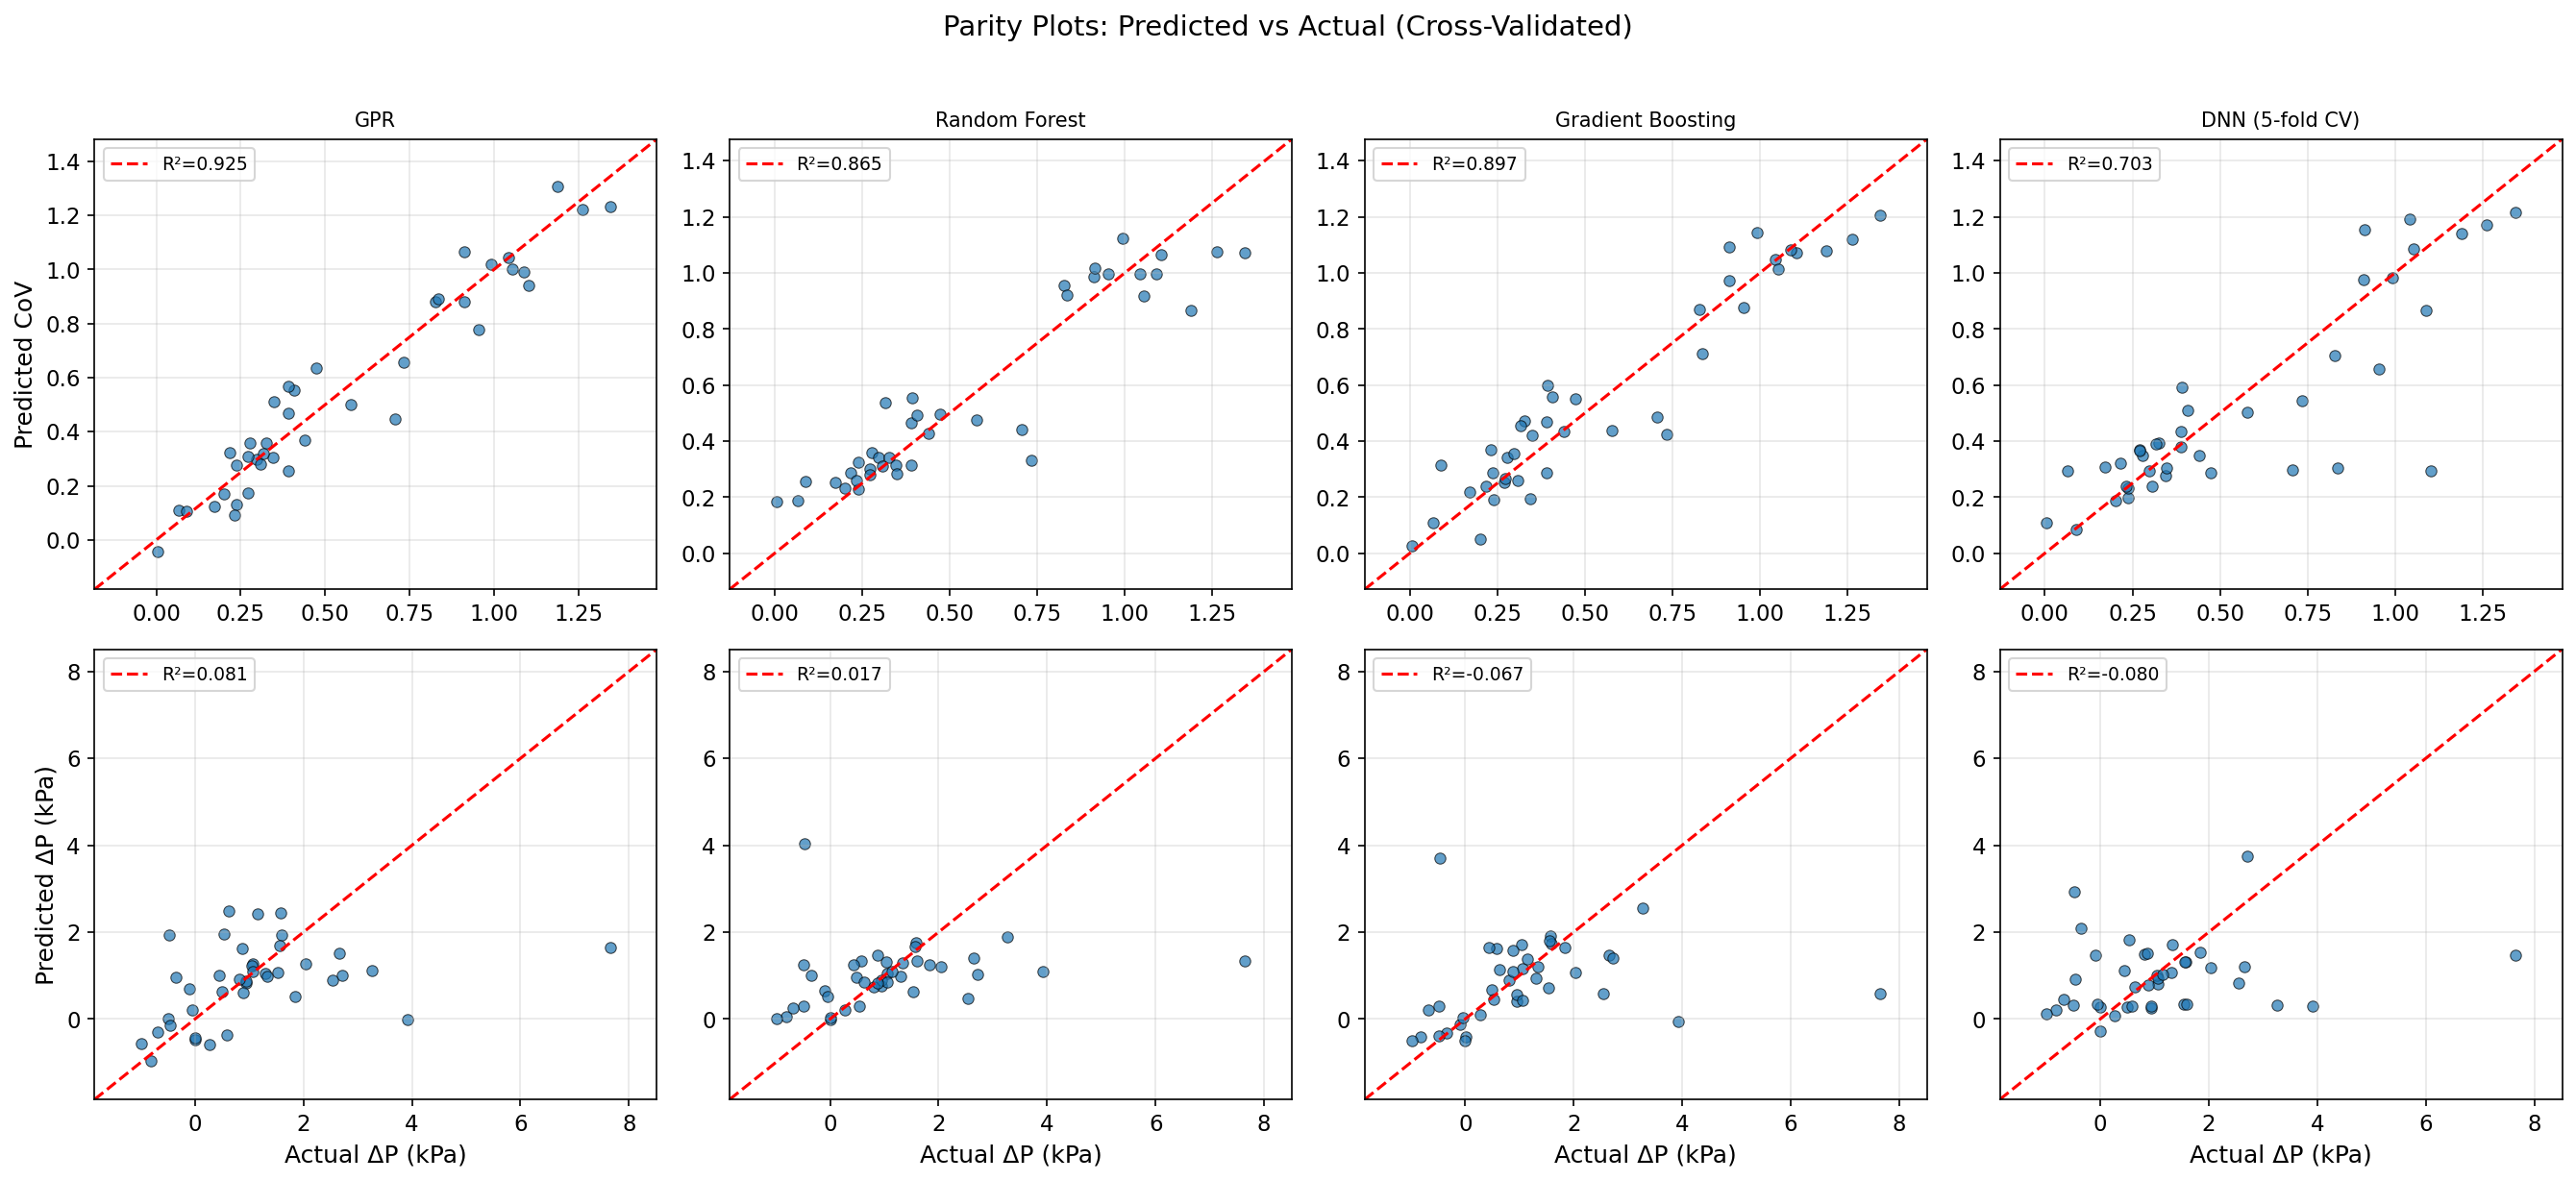
\includegraphics[width=0.85\textwidth]{../doe/surrogate/figures/fig_parity_all_models.png}
   \caption{Parity plots (predicted vs.\ actual) for all four
   surrogates.  GPR provides the tightest \CoV{} scatter.}
   \label{fig:parity_models}
\end{figure}

\subsection{NSGA-II optimisation on GPR surrogate}
\label{sec:nsga2}
The GPR surrogate was fitted on all 40~cases and embedded in
NSGA-II (\(N_{\text{pop}}=200\), 150~generations, SBX crossover
\(\eta_c=15\), polynomial mutation \(\eta_m=20\)).
The optimisation was run independently for top and bottom
injection.  Surrogate predictions are clamped to \(\CoV\ge 0\)
to prevent non-physical extrapolation.

\noindent\textbf{Knee-point designs} (closest to utopia in
normalised objective space):
\begin{itemize}
   \item \textbf{Top injection}: \(\alpha=30^\circ\),
         \(\dD=0.45\), \(\VR=5.82\), \(\HBR=6.0\,\%\)
         \(\Rightarrow\) predicted \(\CoV\approx 0.089\),
         \(|\Delta p|\approx\SI{0.14}{\kilo\pascal}\).
   \item \textbf{Bottom injection}: \(\alpha=90^\circ\),
         \(\dD=0.26\), \(\VR=5.84\), \(\HBR=19.4\,\%\)
         \(\Rightarrow\) predicted \(\CoV\approx 0.048\),
         \(|\Delta p|\approx\SI{0.97}{\kilo\pascal}\).
\end{itemize}
Both knee points maximise \VR{}, confirming SHAP feature-importance
analysis which identifies \VR{} and injection side as the two
dominant features for \CoV.

\begin{figure}[H]
   \centering
   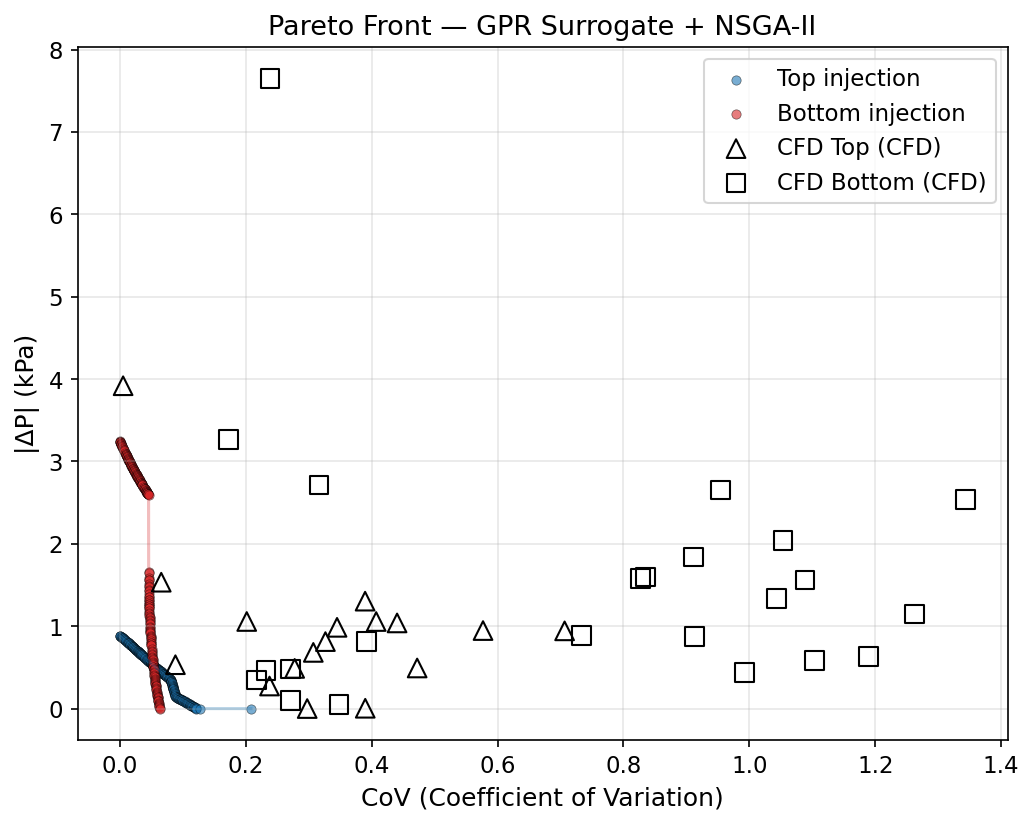
\includegraphics[width=0.78\textwidth]{../doe/surrogate/figures/fig_pareto_front_surrogate.png}
   \caption{NSGA-II Pareto fronts on GPR surrogate, overlaid
   with CFD data (hollow markers).}
   \label{fig:pareto_surrogate}
\end{figure}

\subsection{SHAP feature importance}
\label{sec:shap}
SHAP (SHapley Additive exPlanations) was computed on the GPR
surrogate for \CoV{}.
The three most important features are:
(i)~\textbf{Injection side} (mean \(|\text{SHAP}|=0.28\)):
switching from top to bottom adds \(\sim 0.28\) to \CoV{} on
average.
(ii)~\textbf{\VR} (0.14): higher \VR{} reduces \CoV.
(iii)~\textbf{\HBR} (0.10): higher blending ratio increases
\CoV{} mechanically (more hydrogen to mix).
Angle and \(\dD\) are less important, consistent with the
matched-pair findings.

\subsection{DNN training dynamics}
Figure~\ref{fig:dnn_loss} shows the DNN loss curves.
Training loss converges by epoch~150, but test loss plateaus
near epoch~50, indicating mild overfitting beyond that point.
Early stopping selected the checkpoint at epoch~47.

\begin{figure}[H]
   \centering
   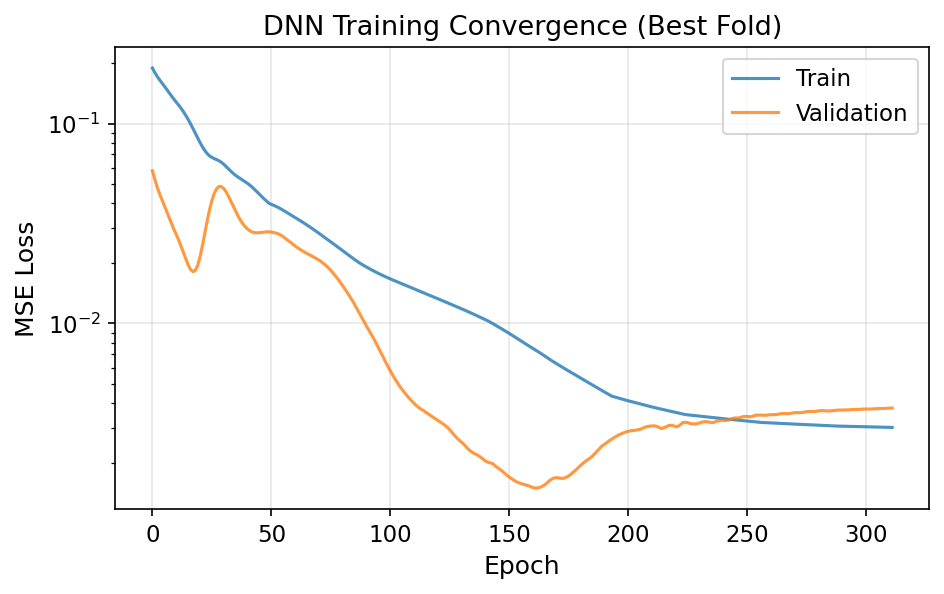
\includegraphics[width=0.65\textwidth]{../doe/surrogate/figures/fig_dnn_training_loss.png}
   \caption{DNN training and validation loss (5-fold).
   Overfitting begins after epoch~50.}
   \label{fig:dnn_loss}
\end{figure}

\subsection{Residuals and error distribution}
Figure~\ref{fig:residuals} shows the residual (predicted minus actual)
distribution for the GPR and Gradient Boosting models.
The GPR residuals are centred at zero with tails extending to
\(\pm 0.2\); the GB shows slightly wider tails.
Neither model exhibits systematic bias.

\begin{figure}[H]
   \centering
   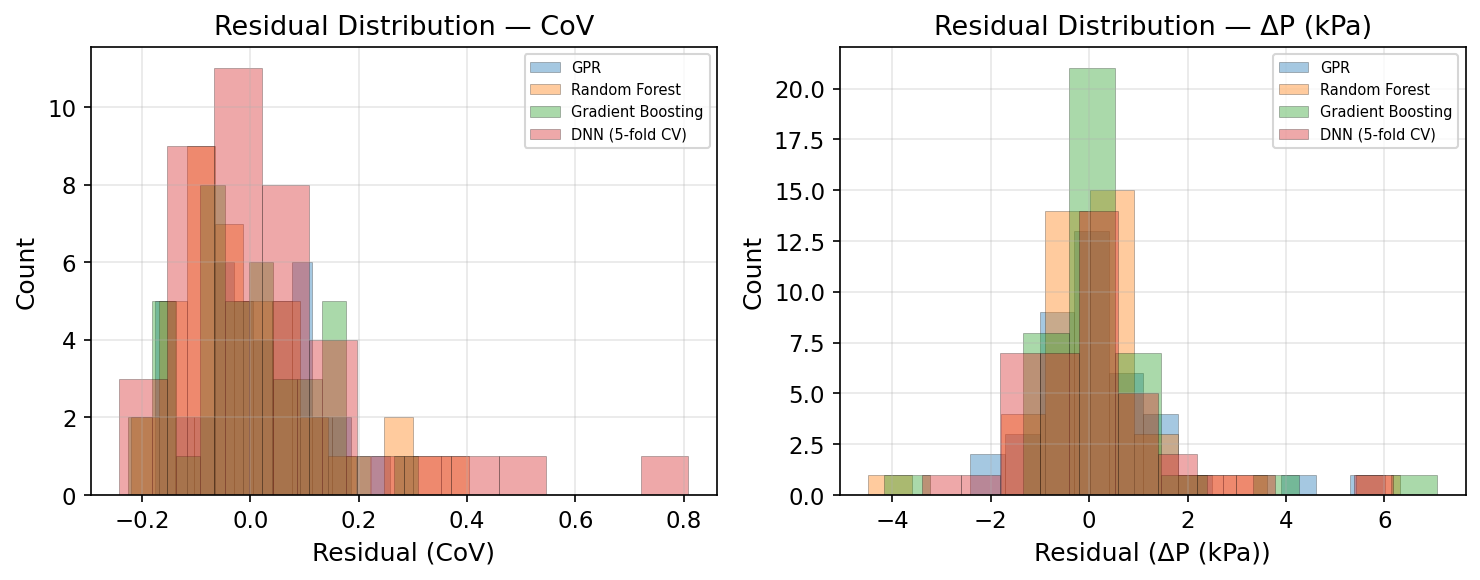
\includegraphics[width=0.78\textwidth]{../doe/surrogate/figures/fig_residuals.png}
   \caption{Residual histograms for GPR and Gradient Boosting
   surrogates (LOO-CV).}
   \label{fig:residuals}
\end{figure}

\noindent
\textbf{Assessment.}
The GPR surrogate for \CoV{} (\(R^{2}=0.93\)) is within the
``usable'' range (\(R^{2}>0.90\)).
The \(\Delta p\) surrogate is not usable; a reliable predictor
requires either longer transient runs or a steady-state solver.
Extending the DoE to the full 420-case plan would provide the
data density needed for the DNN and may also sharpen the
\(\Delta p\) signal enough for the GPR to learn it.

% =====================================================================
%  11. CONCLUSIONS
% =====================================================================
\section{Conclusions and outlook}
\label{sec:concl}

\subsection{What is established}
\begin{enumerate}
    \item A reproducible, angle-agnostic OpenFOAM workflow
    (parametric STL, sliced LHS, slice-based mesh reuse,
    automated post-processing) was built and validated.
    \item For \(90^\circ\) top injection, \CoV{} drops from
    \(0.71\) (\(\VR=0.69\)) to \(0.07\) (\(\VR=3.81\)),
    reproducing literature trends.
    \item For \(30^\circ\) top injection, case~01 reaches
    \(\CoV=0.005\) --- an order of magnitude below the
    \(\CoV\le 0.05\) industrial target.
    \item The \(30^\circ\) vs.\ \(90^\circ\) matched-pair analysis
    (7~pairs) shows median \CoV{} reduction of \(46\,\%\) and
    \(|\Delta p|\) reduction of \(63\,\%\); the tilt
    simultaneously improves mixing and lowers pumping cost.
    \item \textbf{Bottom injection always mixes worse than top.}
    Across 17~matched pairs, top injection achieves lower \CoV{}
    in every single pair (median degradation \(+109\,\%\) at
    \(90^\circ\), \(+324\,\%\) at \(30^\circ\)).  LP-filtered
    \(|\Delta p|\) is comparable across sides, so injection side
    affects only mixing.  Top injection is strictly dominant.
    \item The physical mechanism is buoyancy-driven plume
    restructuring: top injection spreads \Hi{} laterally along the
    crown (large interfacial area, rapid diffusion); bottom
    injection lifts it as a coherent column without spreading.
    \item The power-law \(\CoV=A\,\VR^{b}\) is steepest for
    \(30^\circ\) top (\(b=-1.88\)) and shallowest for
    \(30^\circ\) bottom (\(b=-0.72\)), confirming that top
    injection converts each unit of \VR{} into more mixing.
    \item GPR surrogate achieves \(R^{2}=0.93\) for \CoV{} on
    LOO-CV; \(\Delta p\) is unpredictable (\(R^{2}\approx 0\))
    at current data size due to acoustic noise.
\end{enumerate}

\noindent\textbf{Caveats.}
(i)~The matched-pair set has 7~points per angle comparison;
while the binomial \(p\)-value is significant (\(0.8\,\%\)),
the set does not span the full design space densely.
(ii)~Mesh convergence was verified at one design point; the same
\(\sim\!460\,\mathrm{k}\)-cell baseline is used everywhere.
(iii)~The main-pipe Reynolds number is fixed at one value.

\subsection{Practical recommendation}
\begin{enumerate}
    \item \textbf{Always inject from the top.}
    \item \textbf{Use \(30^\circ\) tilt} rather than \(90^\circ\).
    \item \textbf{Maximise \VR{}} (target \(\VR\ge 2.5\)).
    \item The \(\dD\) effect is secondary in the present range.
\end{enumerate}

\subsection{Outlook}
\begin{itemize}
    \item Extend DoE to the full 420-case plan (5 angles
    \(\times\) 3 \(\dD\) levels \(\times\) 2 sides) for a
    reliable DNN and bi-objective Pareto front.
    \item Run steady RANS (\texttt{rhoSimpleFoam}) or extend
    transient to \(\sim\SI{5}{\second}\) for sharper \(|\Delta p|\).
\end{itemize}

\subsection{Data and code availability}
\label{sec:data_avail}
All code, case templates, post-processing scripts and figure
generators are open-source at
\url{https://github.com/Yash04dsr/MTP-Work}.

% =====================================================================
%  ACKNOWLEDGEMENTS
% =====================================================================
\section*{Acknowledgements}
I thank Prof.~Abhijeet Raj for supervision and guidance; the
Department of Chemical Engineering, IIT Delhi, for computing
resources; and the OpenFOAM community.

% =====================================================================
%  BIBLIOGRAPHY
% =====================================================================
\bibliographystyle{unsrtnat}
\bibliography{bibliography}

\end{document}
